% プロジェクト学習中間報告書書式テンプレート ver.1.0 (iso-2022-jp)

% 両面印刷する場合は `openany' を削除する
\documentclass[openany,11pt,papersize]{jsbook}

% 報告書提出用スタイルファイル
%\usepackage[final]{funpro}%最終報告書
\usepackage[middle]{funpro}%中間報告書

% 画像ファイル (EPS, EPDF, PNG) を読み込むために
\usepackage[dvipdfmx]{graphicx,color}

% ここから -->
\usepackage{calc,ifthen}
\newcounter{hoge}
\newcommand{\fake}[1]{\whiledo{\thehoge<70}{#1\stepcounter{hoge}}%
  \setcounter{hoge}{0}}
% <-- ここまで 削除してもよい

% 年度の指定
\thisYear{2016}

% プロジェクト名
\jProjectName{使ってもらって学ぶフィールド指向システムデザイン}

% [簡易版のプロジェクト名]{正式なプロジェクト名}
% 欧文のプロジェクト名が極端に長い(2行を超える)場合は、短い記述を
% 任意引数として渡す。
%\eProjectName[Making Delicious curry]{How to make delicious curry of Hakodate}
\eProjectName{Field Oriented System Design Learning by Users' Feedback}


% <プロジェクト番号>-<グループ名>
\ProjectNumber{03-A}

% グループ名
\jGroupName{町内会グループ}
\eGroupName{Neighborhood Association Group}

% プロジェクトリーダ
\ProjectLeader{1014237}{伊藤泰斗}{Taito~Ito}

% グループリーダ
\GroupLeader  {1014120}{永井陽太}{Youta~Nagai}

% メンバー数
\SumOfMembers{5}
% グループメンバ
\GroupMember  {1}{1014059}{船木綾香}{Ayaka~Funaki}
\GroupMember  {2}{1014120}{永井陽太}{Youta~Nagai}
\GroupMember  {3}{1014231}{森島帆南}{Honami~Morishima}
\GroupMember  {4}{1014237}{伊藤泰斗}{Taito~Ito}
\GroupMember  {5}{1014253}{横山新}{Arata~Yokoyama}

% 指導教員
\jadvisor{伊藤恵,南部美砂子,奥野拓,木塚あゆみ,原田泰}
% 複数人数いる場合はカンマ(,)で区切る。カンマの前後に空白は入れない。
\eadvisor{Kei~Ito,Misako~Nambu,Taku~Okuno,Ayumi~Kizuka,Yasushi~Harada}

% 論文提出日
\jdate{2016年7月27日}
\edate{July~27, 2016}

\begin{document}
%
% 表紙
\maketitle

%前付け
\frontmatter

% 和文概要
\begin{jabstract}
本プロジェクトでは、フィールドを実際に調査してそこから問題点を見つける。そこで見つかった問題点をICTを活用して解決する。それにより地域・社会に貢献することを目標として活動を行っている。開発手法はアジャイル開発手法を用いる。素早くアプリを開発し、それに対するレビューを受けて問題解決の質をより高いものにしていく。
 我々町内会グループは、陣川あさひ町会をフィールドに設定した。函館市陣川町にある陣川あさひ町会(以下、町会とする)は1200世帯中1000世帯が加盟しており1000人規模のイベントを開催しているなど、積極的に活動をしている2016年5月中旬に実際に陣川あさひ町内会へ現地調査へ行き、どのような問題点があるのか、どのような要望があるのかをヒアリングした。ヒアリングした結果、陣川あさひ町会役員(以降、役員とする)が複数のSNSに投稿するのが大変であることや参加者の管理がうまくいっていないこと、イベントの緊急連絡ができていないという問題点があった。そこから我々が話し合って固めたアプリ案をティーチングアシスタント(以降、TAとする)や担当教員、役員の方々からレビューを受けながら、開発を行った。
5月30日の第1回提案では、役員のイベント開催に関する問題を解決するため、カレンダー表示を中心としたイベント管理アプリケーションの提案をした。次に6月23日の第2回提案では第1回提案を経て更に内容を精査して「イベント作成機能」、「イベント参加申し込み機能」、「イベント通知機能」を提案した。しかし7月8日に行われた中間報告会で、町民の方々に使ってもらうための伝達手段について考慮されていない課題が見つかった。そのため8月6日に催される納涼まつりにて町民に対して、どのようにアプリケーションを導入してもらうかを見当して、レビューをいただく予定である。そして使ってもらって学ぶサイクルを繰り返すことで役員の要望にあったシステムデザインを行っていく。

% 和文キーワード
\begin{jkeyword}
陣川町, 陣川あさひ町会, アジャイル開発, アプリケーション, イベント, レビュー, システムデザイン
\end{jkeyword}
\bunseki{伊藤泰斗}
\end{jabstract}
​
%英語の概要
\begin{eabstract} Abstract in English.
In this project, at first, we investigate on the field and find problems from field survey. We solve the problems found from field survey by ICT. Then we have action with the goal of contributing to an area. We use Agile development process which is a software development technique. We do swift app development, and develop higher quality app by being reviewed for it. 
% 英文キーワード
\begin{ekeyword}
Keyrods1, Keyword2, Keyword3, Keyword4, Keyword5
\end{ekeyword}
\bunseki{伊藤泰斗}
\end{eabstract}


\tableofcontents% 目次


\mainmatter% 本文のはじまり

%背景・目的
\chapter{背景・目的}

\section{陣川町について}
陣川町は北海道函館市にあり(図1とか)、人口はおよそ3,300人の町である。
陣川町には「陣川あさひ町会」がある。
町会は陣川町の1,200世帯中約1,000世帯が加入している。
夏には参加者が約1,000人にもなる納涼まつりや
冬にはウィンターフェスティバルを行うなど積極的に活動している。
また、これらのイベント情報を多くの人に知らせる為に
町会役員がFacebookとLINE@を使い発信している。
しかし、積極的にイベントを開催する上でで様々な問題を抱えている。
\bunseki{船木綾香}

\section{町会が抱える問題}
町会のイベントを開催する上での問題点は主に以下の6つである。
\begin{itemize}
    \item 情報内容に関する問題
    \begin{itemize}
        \item FacebookやLINE@ではイベントに関するお知らせはできるが、
              開催予定のイベントを一覧で見れない。
    \end{itemize}
    \item 情報伝達手段に関する問題
    \begin{itemize}
        \item イベントの情報をFacebookとLINE@に同一の内容を発信する手間がかかる。
        \item 町民のイベント申し込み方法が電話、FAX、メールの3つあり、イベント参加者の管理に手間がかかる。
        \item Facebookでは個人情報が漏れてしまうため参加申し込みができない。
        \item 役員だけで共有したい情報を町民に知られずに共有することがFacebookやLINE@ではできない。
    \end{itemize}
    \begin{itemize}
        \item イベント当日が悪天候の場合、参加者全員に対してイベントの中止、
              延期などの連絡を迅速に行うことができない。
    \end{itemize}
\end{itemize}
このように、町会はイベントを開催する上で様々な問題を抱えている。
\bunseki{船木綾香}

\section{目的}
本グループでは「陣川あさひ町会のイベント開催に関する問題を解決するサービスの提供をする」ことを目的とした。
1.2の通り、町会ではイベントを開催する上で様々な問題がある。
そこで本グループではそれらの問題を解決するアプリケーションを開発する。
\bunseki{船木綾香}


%目的
%\chapter{目的}
​
\section{このグループの目的}%例:レビュー内容
% 必要ならここに大見出しの内容
%必要なら下のsubsectionを用いて小見出しをつかう
%\subsection{ここに小見出し}%:発表技法について
本グループでは「陣川あさひ町会のイベント開催に関する問題を解決するサービスの提供をする」ことを目的と設定した。前述の通り、陣川あさひ町会ではイベントを開催する上でさまざまな問題がある。そこで本グループではそれらの問題を解決するアプリケーションを開発する。
\bunseki{船木綾香}


%開発プロセス
\chapter{開発プロセス}

\section{前期第1プロセス}

\subsection{ヒアリング}
我々は町会の置かれている現状を明らかにするため,
5月12日に町会の会長, 副会長, 総務部長, 会計部長, 青少年育成部副部長に対して,
我々は学部3年生5名とTA5名と教員4名でヒアリングを行った.
町会役員から\ref{problems}で述べたイベント開催に関する問題と以下の要望が明らかになった.

\begin{itemize}
\item 開催予定のイベント一覧をカレンダーで表示して欲しい.
\item iOSのアプリケーションを作って欲しい.
\item 幅広い年代の人が使いやすいUIにして欲しい.
\item 町会の役員の数を増やすため, 町内会を知ってもらいたい.
\item イベント発信をした際に通知できる機能が欲しい.
\item イベントスケジュールでイベントの削除, 作成, 更新ができるようにして欲しい.
\item 行事をタップしたらそのまま参加申し込みフォームに遷移して欲しい.
\item 保護者の方の確認を得るためのポップアップ機能が欲しい.
\item イベントで不参加になった人が分かるようにして欲しい.
\end{itemize}

我々は, これらの要望を取り入れつつ問題を解決するアプリケーションを開発することとした.
\bunseki{永井陽太}


\subsection{アプリケーションアイデアの考案}
\ref{problems}で述べた問題と町会の要望を分析した結果, イベントに関する内容のものが多かった.
そこでイベントに関係する3つの問題を解決することとした. 問題は
「FacebookやLINE@ではイベントに関するお知らせはできるが, 開催予定のイベントを一覧で見れない」
「Facebookでは個人情報が漏れてしまうため参加申し込みができない」
「役員だけで共有したい情報を町民に知られずに共有することがFacebookやLINE@ではできない」の3つである.
これらの問題を解決するために, 開催予定イベントのカレンダー表示機能,
イベントへの参加申し込み機能, 参加申し込み者の情報を役員のみが見ることのできる機能,
役員のみが役員会議などのイベント情報を見ることのできる機能を考案した.
アプリケーションアイデアの一部であるイベントカレンダー画面(図\ref{calender}),
参加フォーム画面(図\ref{joinform}), イベント作成画面(図\ref{create_event.old})を以下に示す.

\newpage
\begin{figure}[h]
    \begin{tabular}{ccc}
      %---- 最初の図 ---------------------------
      \begin{minipage}[t]{0.33\hsize}
        \centering
        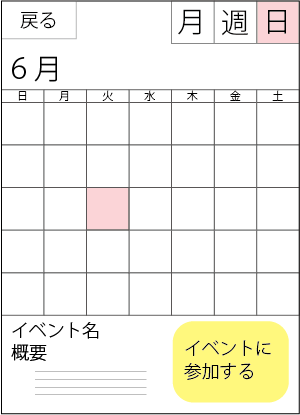
\includegraphics[keepaspectratio, scale=0.4]{process_figures/calender.png}
        \caption{イベントカレンダー画面}
        \label{calender}
      \end{minipage} &
      %---- 2番目の図 --------------------------
      \begin{minipage}[t]{0.33\hsize}
        \centering
        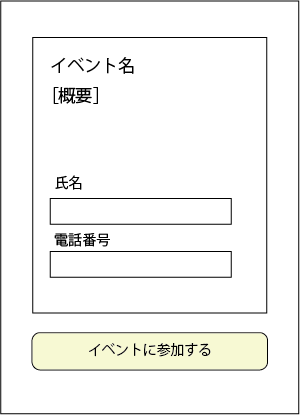
\includegraphics[keepaspectratio, scale=0.4]{process_figures/joinform.png}
        \caption{参加フォーム画面}
        \label{joinform}
      \end{minipage}
      %---- 3番目の図 --------------------------
      \begin{minipage}[t]{0.33\hsize}
        \centering
        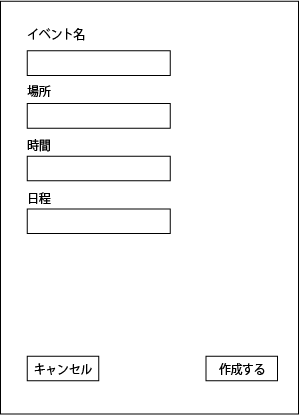
\includegraphics[keepaspectratio, scale=0.4]{process_figures/old_create_event.png}
        \caption{イベント作成画面}
        \label{create_event.old}
      \end{minipage}
      %---- 図はここまで ----------------------
    \end{tabular}
\end{figure}
\bunseki{永井陽太}

\subsection{第1回提案}
\label{first_review}
5月30日に我々が考えたアプリケーションの画面イメージを町会に提案した.
その結果, iOS, Android, Webアプリケーションの3つに対応可能なアプリケーション開発を行うことが決定した.
また, 我々の考案したアプリケーションイメージについて, レビューで3つの要望を得た.
1つ目は, イベント参加者の名簿を市役所に提出する際に参加者の情報として「名前」「性別」「年齢」「住所」「電話番号」が必要なので,
図\ref{joinform}の入力フォームに5つの情報を追加して欲しいという要望である.
2つ目は, アプリケーションをインストールした人が, すぐイベントを確認できるように起動時の画面はログイン画面にしないで欲しいという要望である.
3つ目は, 図\ref{create_event.old}に「定員」の項目を追加して欲しいという要望である.
\bunseki{永井陽太}

\section{前期第2スプリント}

\subsection{第1回月例レビュー会}
月例レビュー会とは, プロジェクト内で, 3つのチームが現在の進捗報告と今後の展望を発表し, その発表内容に対して担当教員, TA, 他チームのメンバーからレビューを受ける会である.
ここで我々は, 現在のアプリケーションアイデア, つまり, 役員と町民でイベントカレンダーを共有する機能で本当に問題を解決できているのかと教員より指摘を受け,
\ref{first review}にうけたレビュー内容も考慮し, アプリケーションについて再考し改善を図った.


\subsection{アプリケーションアイデアの改善}
改善の結果, カレンダーを用いて開催予定のイベントを表示するのではなく,
開催予定のイベントを直近のものから順にリスト表示することにした.
なぜなら, カレンダー表示では来月の予定などがひと目で確認することができないからである.
アプリケーションアイデアの一部であるイベントリスト画面(図\ref{eventlist}),
イベント作成画面(図\ref{new_create_event}), 参加者リスト画面(図\ref{joinedlist})を以下に示す.

\newpage%苦肉の策
\begin{figure}[h]
    \begin{tabular}{ccc}
      %---- 最初の図 ---------------------------
      \begin{minipage}[t]{0.3\hsize}
        \centering
        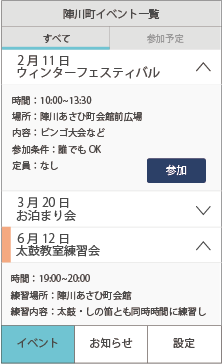
\includegraphics[keepaspectratio, scale=0.5]{process_figures/eventlist.png}
        \caption{イベントリスト画面}
        \label{eventlist}
      \end{minipage} &
      %---- 2番目の図 --------------------------
      \begin{minipage}[t]{0.3\hsize}
        \centering
        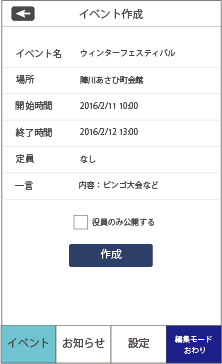
\includegraphics[keepaspectratio, scale=0.5]{process_figures/new_create_event.png}
        \caption{イベント作成画面}
        \label{new_create_event}
      \end{minipage}
      %---- 3番目の図 --------------------------
      \begin{minipage}[t]{0.3\hsize}
        \centering
        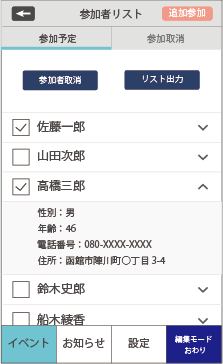
\includegraphics[keepaspectratio, scale=0.5]{process_figures/joinlist.png}
        \caption{参加者リスト画面}
        \label{joinedlist}
      \end{minipage}
      %---- 図はここまで ----------------------
    \end{tabular}
\end{figure}
\bunseki{永井陽太}

\subsection{第2回提案}
6月23日に我々は町会に対して改善したアプリケーションイメージを提案した.
その結果, 画面ごとにレビューしてもらい詳細な要望を受けた.
具体的には, 図\ref{eventlist}でイベントをタップすると画面いっぱいにイベントの詳細情報が表示されるようにして欲しいという要望,
図\ref{new_create_event}にアプリケーションの所有者全員に通知するか, しないかの項目を設けて欲しいという要望である.
また, 町民が利用したくなるようなコンテンツを追加して欲しいという要望も得た.
過去のイベントの写真が確認できるWebページとアプリケーションとリンクさせることが例として挙げられる.
\bunseki{永井陽太}

\section{前期第3スプリント}

\subsection{中間発表}
%----中間発表の内容-----------------
7月8日に行われた中間発表では, 各グループが行ってきた活動を詳細に伝え, 後期の活動に活かせるレビューをもらうことを目的とした.
そのため全体ポスター2分, 各グループのポスターとデモを含めた発表を12分間並行して発表を行った.
\bunseki{伊藤泰斗}

\subsubsection{発表方法についての評価と振り返り}
以下に, 中間発表会で行ったアンケートの「発表技術について」の項目から, メンバ間で精査した結果, 最終成果発表にも取り入れたいコメントを抜粋した.
\begin{itemize}
  \item デモがプロトタイプであることを伝えないと, 実装したものだと勘違いしてしまう.
  \item もう少しスラスラ話せていたら分かりやすかったと感じた.
\end{itemize}
    上記より, 伝える情報とポスターセッションの練習の不足が伺える.
    しかし, 「とても喋りに安定感があるなと感じた」との評価も受けた. 最終成果発表の際にはすべて開発したアプリケーションでデモを行い,
    ポスターセッションをする人全員がスラスラと話せるくらいに練習を行っていく.

\subsubsection{発表内容についての評価と反省}
    「発表内容について」の項目から後期の開発や発表において考慮すべきコメントを抜粋した.
\begin{itemize}
  \item 陣川町民に使ってもらうためのプロモーションの方法を考えたほうが良い
  \item クーポンなど, ユーザを得る工夫が欲しい
  \item ユーザにより沿って開発していく中で生起した出来事を大切に記述して欲しい
\end{itemize}
    上記より, 2つの見落としが伺えた. 1つ目はユーザに使ってもらうための考慮をしていなかったことである.
    メンバ全員が使ってもらえることを前提として考えていることである. しかし実際には使ってもらえることは前提ではないため,
    どのようにして使ってもらうのかを考える必要がある. 2つ目は, 本アプリケーションにユーザにとって魅力的な優位性が必要であることである.
    認知されていてもユーザにとって使いたいものでなければ使ってもらうことができない. そのため, 最終成果発表までにプロモーションの方法を考え,
    使ってもらうための工夫を本アプリケーションに追加することでユーザを獲得していきたい.
\bunseki{伊藤泰斗}


\subsection{第1回集中実装}
夏季休業期間中に, じぷりの主要な機能の内の「イベントの編集・削除機能」, 「お知らせの削除機能」, 「イベントへの参加申し込み機能」を実装した.
%----集中開発の内容-----------------

\section{後期第1スプリント}
\subsection{後期活動開始}
バックログの導入
ルールの制定
じぷりの進捗確認

\section{後期第2スプリント}
\subsection{じぷりデザインの改善}
\subsection{町会打ち合わせ}
\subsection{第2回月例レビュー会}

\section{後期第3スプリント}
\subsection{アカデミックリンク}
\subsection{町会打ち合わせ}

\section{後期第4スプリント}
\subsection{町会打ち合わせ}
\subsection{最終成果発表}


%開発準備
\chapter{開発準備}

\section{開発に利用したツールとその経緯}%例:レビュー内容
%必要ならここに大見出しの内容
%必要なら下のsubsectionを用いて小見出しをつかう
\subsection{Monaca}%:発表技法について
iOSとAndroidの両方のプラットフォームでアプリケーションを使いたいという町会の要望を叶えるために, HTML5ハイブリッドアプリを開発することとした. iOSとAndroidには, 「WebView」と呼ばれるブラウザの機能を持つコンポーネントが組み込まれている\cite{book_about_monaca}. HTML5ハイブリッドアプリとは, 「WebView」にHTMLとCSS, JavaScriptを用いて開発するアプリケーションである\cite{book_about_monaca}. また, HTML5ハイブリッドアプリの開発ツールのなかからMonacaを選択した. MonacaはCordovaというオープンソースのフレームワークを利用している\cite{book_about_monaca}. また, MonacaにはMonacaクラウドIDE, Monaca Localkit, Monaca CLIの3種類の開発環境が存在する\cite{book_about_monaca}. MonacaクラウドIDEは, インターネットクラウド上で開発するため個人の開発環境に依存しない\cite{book_about_monaca}. Monaca Localkitは, MonacaクラウドIDEとは異なり, 各メンバごとにローカルでの開発を可能とする\cite{book_about_monaca}. Monaca CLIは, MonacaクラウドIDEが提供するサービスを, コマンドライン形式で利用することを可能にする\cite{book_about_monaca}. いずれの開発環境においても, Monacaデバッカーを用いて, デバックを行う(図\ref{fig:image_monaca}). 

\begin{figure}[h]
  \begin{center}
  %\begin{flushleft}
    \begin{tabular}{c}

      % 1
      \begin{minipage}{0.7\hsize}
        \begin{center}
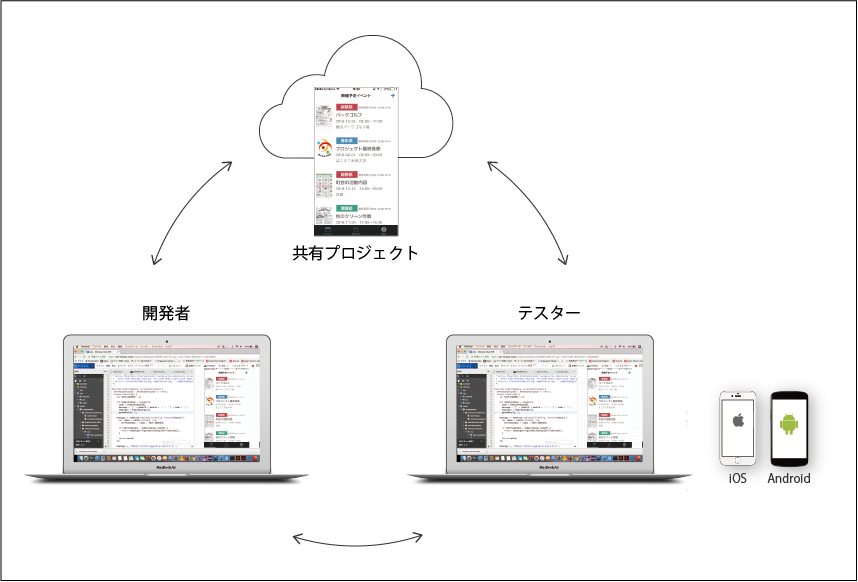
\includegraphics[width=10cm]{monaca_overview.eps}
          \hspace{1cm} %(a)観光スポットの紹介
        \end{center}
      \end{minipage}

    \end{tabular}
    \caption{Monacaでの開発イメージ\cite{monaca_debugger}}
    \label{fig:image_monaca}
  \end{center}
  %\end{flushleft}
\end{figure}

\subsection{ニフティクラウド mobile backend}%:発表技法について
本アプリケーションの各情報を保存する場所として, mBaaSの1つであるニフティクラウド mobile backend(以下, NCMBとする)を使用した. 使用した理由として, 以前このサービスを利用したことがあること, 他のmBaaSと比べて無料で利用可能な機能多いことが挙げられる. mBasSとは, サーバーの開発, 運用を必要とせずユーザから直接見えない部分の機能をアプリケーションに実装することを可能にするサービスである\cite{about_mbaas}. NCMBは, プッシュ通知, 会員管理と認証, SNS連携などの機能\cite{price_mbaas}を提供しているサービスである(図\ref{fig:image_mbaas}).

\begin{figure}[htbp]
%\begin{flushleft}
  \begin{center}
    \begin{tabular}{c}

      % 1
      \begin{minipage}{0.7\hsize}
        \begin{center}
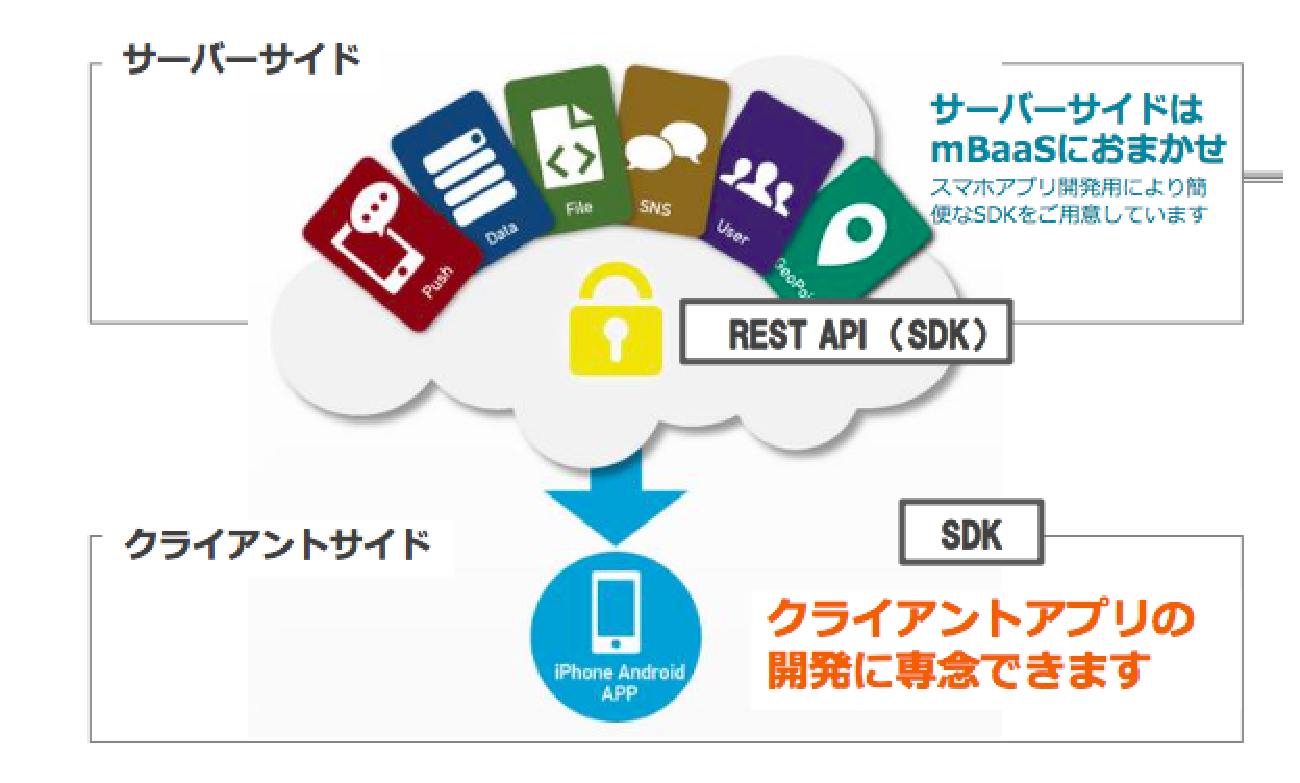
\includegraphics[width=10cm]{ncmb_overview.eps}
          \hspace{1cm} %(a)観光スポットの紹介
        \end{center}
      \end{minipage}

    \end{tabular}
    \caption{ニフティクラウド mobile backendのサービス内容\cite{intro_mbaas}}
    \label{fig:image_mbaas}
  \end{center}
  %\end{flushleft}
\end{figure}


\subsection{Git/GitHub}%:発表技法について
ソースコードのバージョン管理ツールとして, Git/GitHubを使用した. Gitはファイルの変更履歴をリポジトリと呼ばれる場所に保存する. そのため, 一度編集したファイルを過去の状態に復元することや, 編集箇所を表示することが可能となる\cite{book_about_github}. リポジトリの種類は, メンバのローカルPC内に存在するローカルリポジトリと, インターネット上に存在するリモートリポジトリの2種類である\cite{monkey_git}. リモートリポジトリでは, 各メンバのファイルの変更履歴を保存し, 共有する事が可能である. GitHubは, リモートリポジトリを提供するサービスの1つである. これにより, 複数のメンバで同時に開発を進めることが可能となった.


\subsection{Redmine}%:発表技法について
タスク管理ツールとして前期は, Redmineというオープンソースソフトウェアを使用した. Redmineでは, 発生したタスクごとにチケットと呼ばれるものを発行する. その後, タスクの進捗に合わせて各チケットを新規, フィードバック, 進行中(着手), 進行中, 進行中(終了間際), 作業終了, レビュー中, 完了, 却下の9段階に分ける. また, チケットには担当者を指定し, チケットが更新される度に通知が来るようにウォッチャーと呼ばれるものに各メンバを設定する. これにより, 各メンバのタスクの進捗状況を把握することが可能となった.しかし,機能の多さからなる操作の複雑さや,チケットの変更を受動的に知ることができないといった理由から,後期は使用を見送った。

\subsection{Trello}%:発表技法について
タスク管理ツールとして, 後期からTrelloを使用した. Trelloでは, タスクひとつひとつを「カード」として登録し, 「ボード」と呼ばれる場所で管理する\cite{Trello}. その後, todoやdoneなど好きな名前で「リスト」を作成し, 進捗状況に合わせて「カード」を移動することで, 進捗を管理する\cite{Trello}(図\ref{fig:image_trello}). また, ボードは個人で使うこともチームで共有することもできる\cite{Trello}. 完了した「カード」はアーカイブする. さらに, 「カード」が移動されると, チームで使用している連絡ツールに通知が来るように設定をした. これにより, Redmineよりも迅速に進捗を把握することができた. また, 通知が来た後そのまま連絡ツールで, 話し合いをすることもできた.
%参照先 https://seleck.cc/610
\begin{figure}[htbp]
%\begin{flushleft}
  \begin{center}
    \begin{tabular}{c}

      % 1
      \begin{minipage}{0.7\hsize}
        \begin{center}
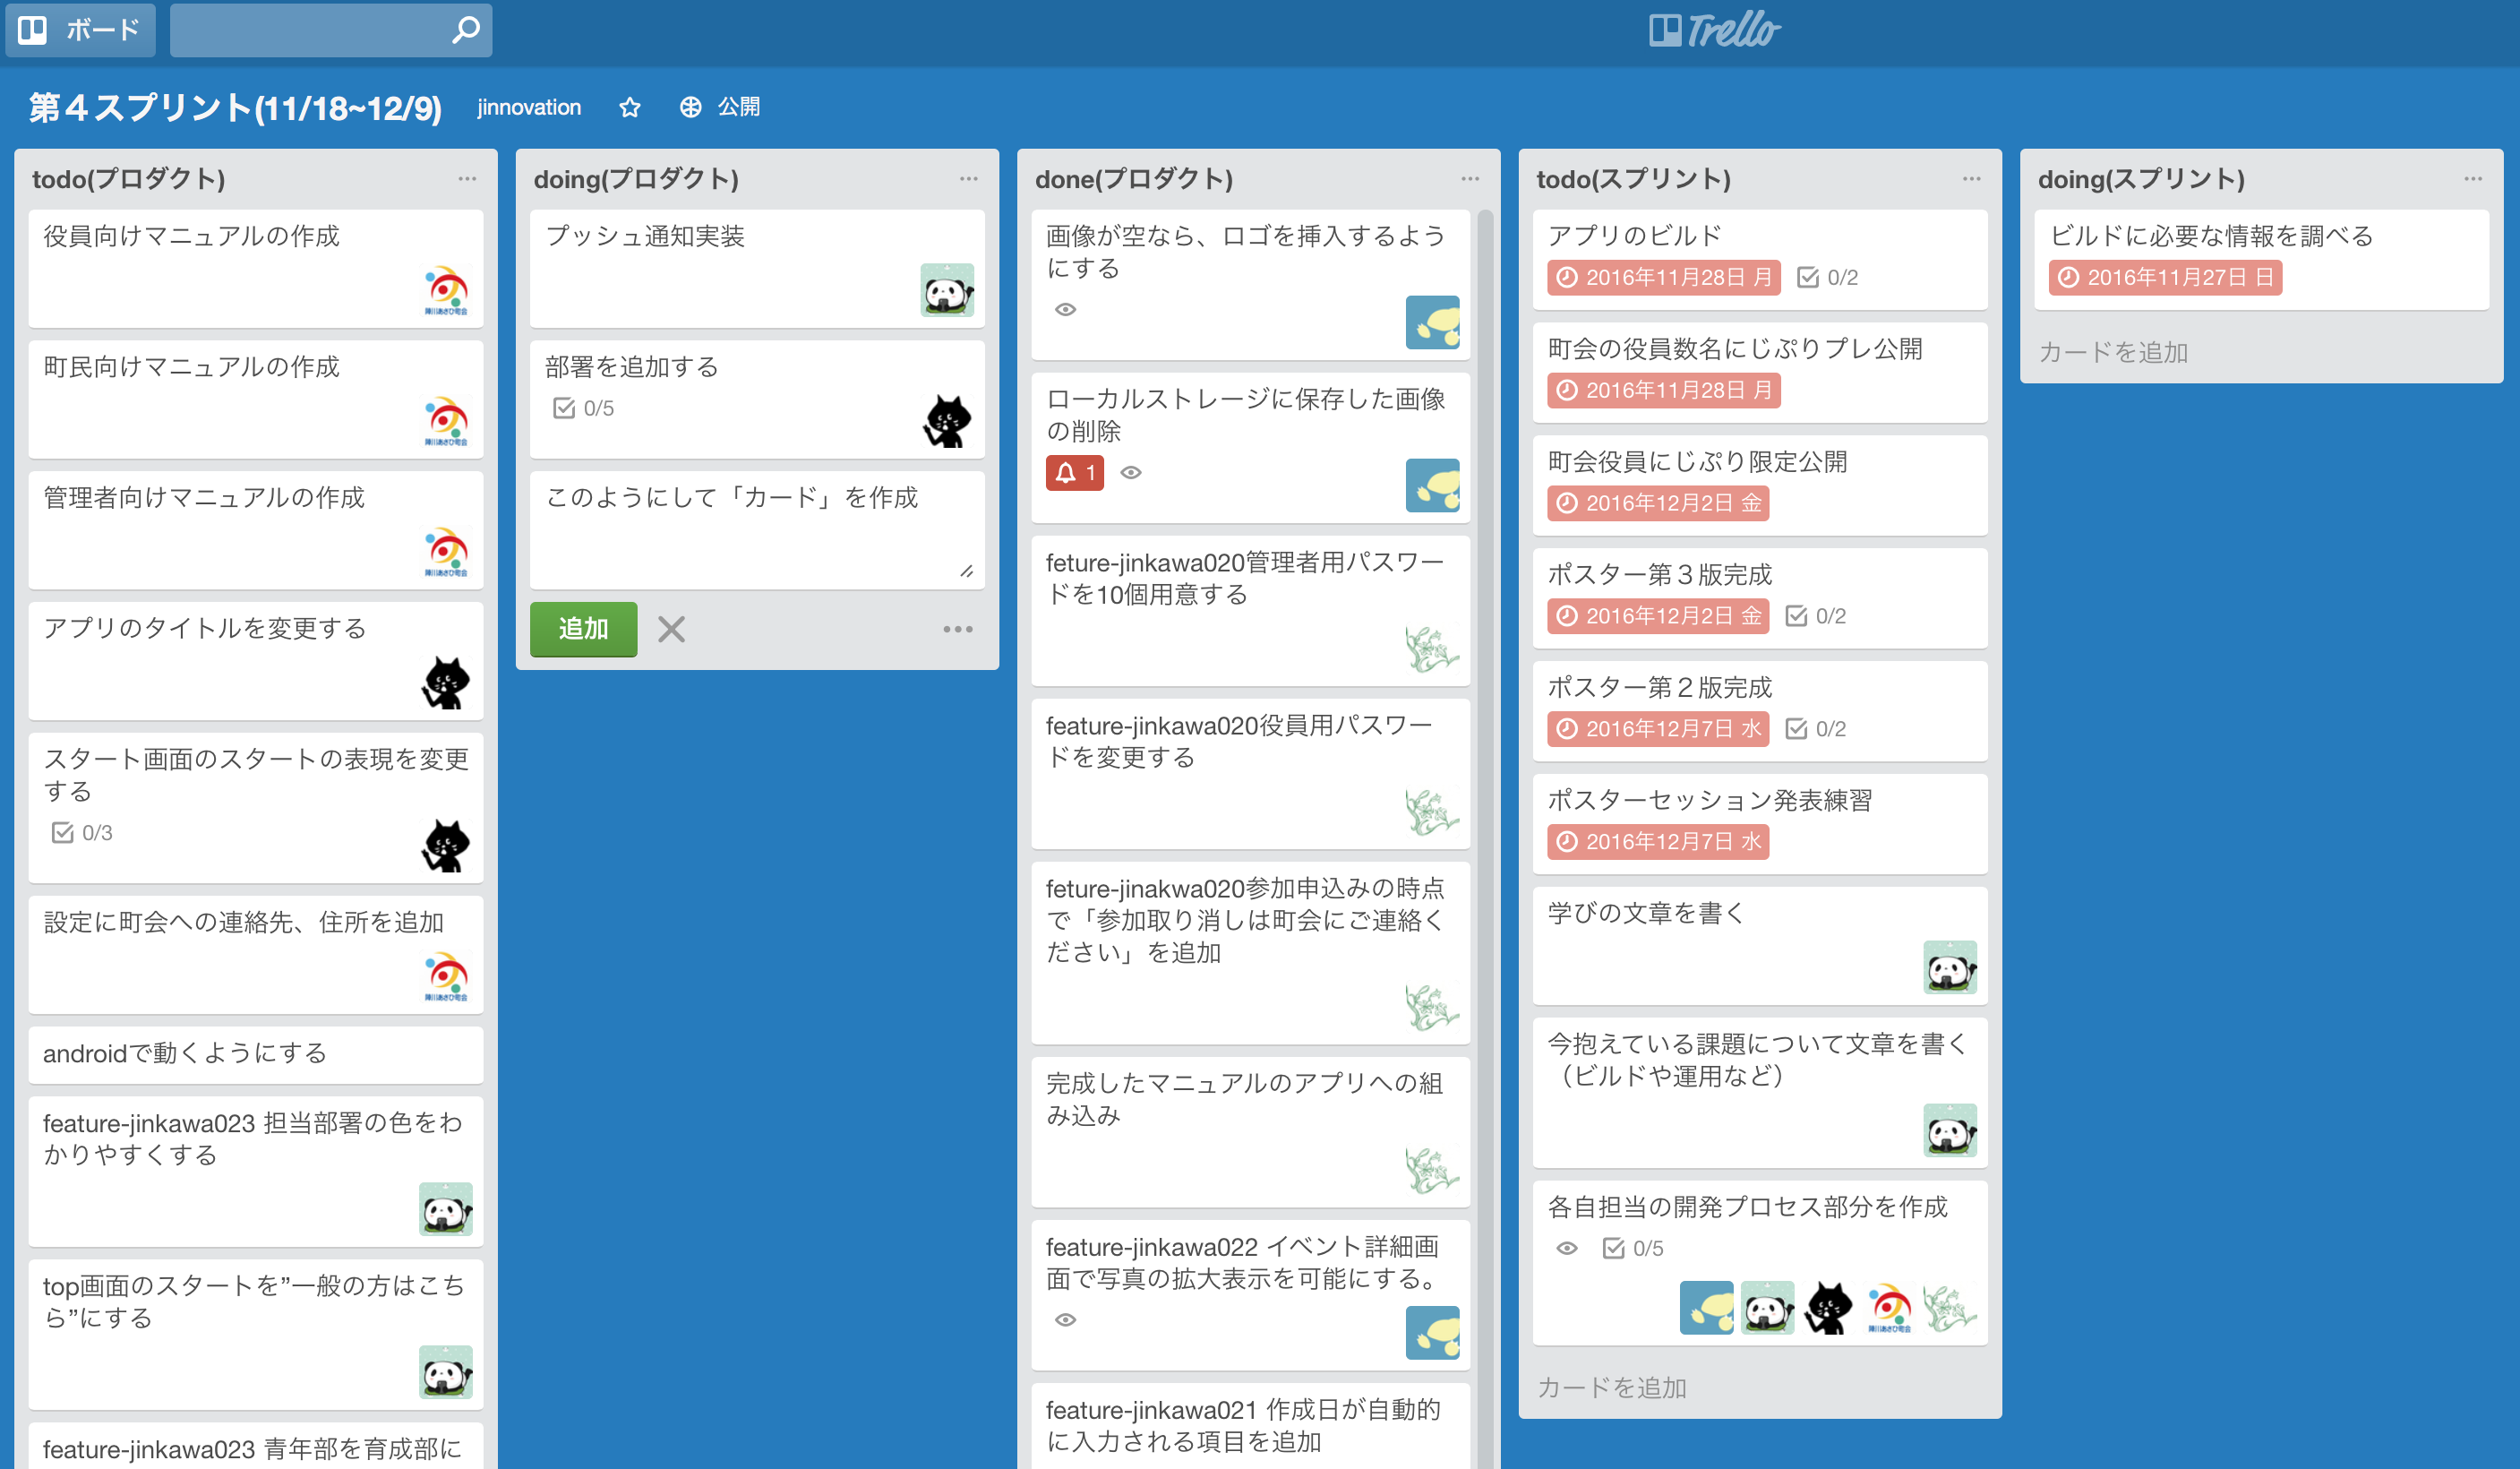
\includegraphics[width=10cm]{about_trello.png}
          \hspace{1cm} %(a)観光スポットの紹介
        \end{center}
      \end{minipage}

    \end{tabular}
    \caption{実際に使用したTrelloの「ボード」}
    \label{fig:image_trello}
  \end{center}
  %\end{flushleft}
\end{figure}

\subsection{Adobe Illustrator}%:発表技法について
ポスター作成と開発するアプリケーションのイメージ図の作成にAdobe Illustratorを使用した. Adobe Illustratorはイラストやポスターなどデザインを描画するソフトウェアの1つである.

\bunseki{横山新}

\section{環境構築}%例:レビュー内容
Monacaの3種類の開発環境の中から, オフラインで作業する可能性があることと普段使い慣れているエディターで開発することが望ましいため, Monaca CLIを選択した. Monacaの公式Webサイト\cite{tutorial_monaca_CLI}を見ながら, Monacaアカウントの作成, Monaca CLIのインストール, コマンドラインからMonacaへのログイン, 新規プロジェクト作成の順で環境構築を行った. GitHubについては, リモートリポジトリに機能やバグの修正ごとにブランチを作成し, そこにプッシュするようにした. また, リモートリポジトリにdevelopブランチを作成した. このdevelopブランチは, 各ブランチの内容をマージするためのブランチである. このdevelopブランチを作成した理由は, 単体テストを終えた各ブランチの内容をmasterブランチにマージする前に, developにマージすることで, 結合テストを行うためである. また, masterの内容を常に安定した状態に保つという役割も担っている. 前期に使用したRedmineは, 担当教員よりすでに構築済みのものを提供していただいた. 原則ウォッチャー\cite{Redmine}は, メンバ全員を登録することとした. 後期に使用したTrelloは, 各自アカウントを作った後, 共有するボードを作成した. その後, チームで利用している連絡ツールと連携させた.

\bunseki{横山新}


%じぷりについて
\chapter{「じぷり」について}

\section{「じぷり」の概要\label{sec:app_overview}}
%例:レビュー内容
%必要ならここに大見出しの内容
%必要なら下のsubsectionを用いて小見出しをつかう
%\subsection{ここに小見出し}%:発表技法について
本プロジェクトで開発しているHTML5ハイブリッドアプリケーション「じぷり」は, 町会が企画, 運営するイベント情報の発信, 発信されたイベントへの参加申し込み, 雨天延期などの町会役員による緊急連絡が可能となるアプリケーションである. このアプリケーションの名称は, 「陣川」という地域の名称と, 「アプリケーション」を組み合わせたものである. じぷりの目標は, 町会のイベント開催に関する問題を解決することである. 主な使用場面は新規イベントの開催が決定してから, 当日のイベント終了までを想定している. 既存の他のアプリケーションと比較した際の優位性として, 1年間を通して何度も町会と打ち合わせを重ねてきたため, 町会の求めていることだけを「じぷり」では組み込んでいる. 求めていることとは, 機能だけではなく, UIの面も含まれている. 詳細は次節以降で述べていく. 「じぷり」では対象とするユーザを, 町民, 役員, 管理者に属性分けをした. 管理者とは, 役員の中でもスマートフォンの操作に慣れている人のことである. このようにした理由は, 町会にヒアリングをした際に, 役員の中には上手くアプリケーションを操作できないと考えられるユーザがいるため, 誤った情報を発信するといったリスクを挙げられたからである. そのため町会と相談した上で, 管理者を誰にするかを決めた. 「じぷり」では, アプリケーションの起動時に, ユーザが町民, 役員, 管理者のいずれかであるかを選択する. その結果からじぷりは, 町民が利用する「一般モード」か, 役員が利用する「役員モード」か, 管理者が利用する「管理者モード」に画面の遷移を行う. 「一般モード」では, イベント情報とお知らせの閲覧と, イベントへの参加申し込みを行うことができる. 「役員モード」では, 「一般モード」に加えて役員会議など役員以外にとって必要のない情報も閲覧できる. 「管理者モード」では, イベントの管理機能,お知らせの管理機能, 参加者管理機能も行うことができる. 次節より「じぷり」の各機能について詳しく記述していく.

\section{イベント管理機能}%例:レビュー内容
\subsection{イベント管理機能の概要}%:発表技法について
イベント管理機能とは「管理者モード」の場合のみ利用可能な機能であり, イベント情報の発信と発信した情報の編集, 削除を可能としている. イベント管理機能を実装した理由は, イベントの情報をFacebookやLINE@など複数のサービスを使用して発信していた従来の方式から, じぷり1つですべてを賄うことを可能とするためである.

\subsection{イベント情報の発信機能}%:発表技法について
\label{subsec:event_add}
イベント一覧リスト画面(図\ref{tab:trans_event}(a))からプラスの形をしたボタンを押すと, 発信するイベント情報の入力画面(図\ref{tab:trans_event}(b))に遷移する. この発信画面では, 入力する情報の属性としてイベント告知用の画像, 担当部名, イベント名, 日程, 場所, 開始時間, 終了時間, 定員, 詳細, 申込締切日, 役員のみに公開の11個に分けた. 役員のみに公開とは, 役員会議など町民にとっては知る必要のないイベント情報を判別するために設けた. また, イベント一覧リスト画面(図\ref{tab:trans_event}(a))を見た時に, ひと目でどの部が担当しているのかをわかるようにしてほしいとの要望を受けたため, 担当部別に色を付けた. これは, \ref{sec:app_overview}節(\pageref{sec:app_overview}ページ)で記述した「じぷり」が持つ優位性の1つである. これら11個の属性は, ヒアリングを通して定まったものである. 情報を入力した後画面下の作成ボタンを押すことでイベント情報を発信することが可能となる.

\begin{figure}[htbp]
  \begin{center}
    \begin{tabular}{c}

      % 1
      \begin{minipage}{0.33\hsize}
        \begin{center}
        {\setlength{\fboxsep}{0cm}\fbox{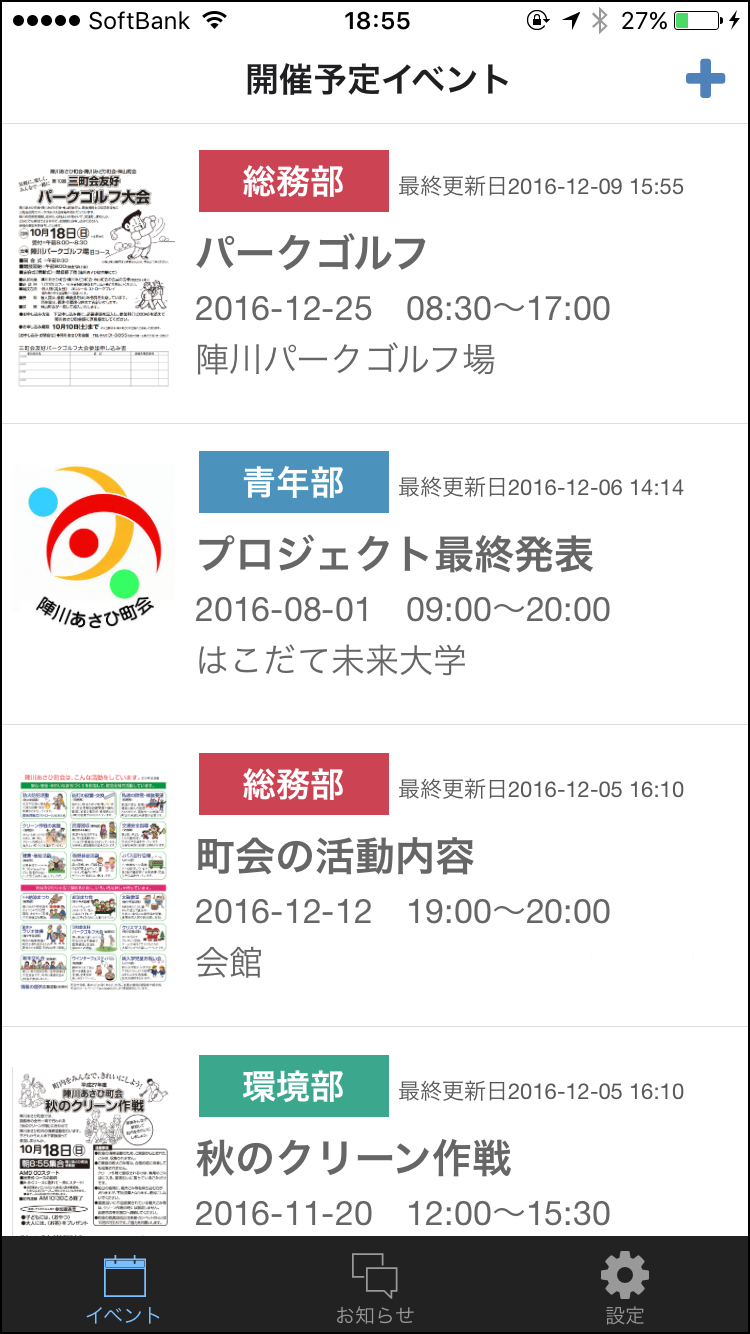
\includegraphics[width=4cm]{event_list.png}}}
          \hspace{1cm} %(a)観光スポットの紹介
          {\footnotesize (a)イベント一覧リスト画面}
        \end{center}
      \end{minipage}

      % 2
      \begin{minipage}{0.33\hsize}
        \begin{center}
        {\setlength{\fboxsep}{0cm}\fbox{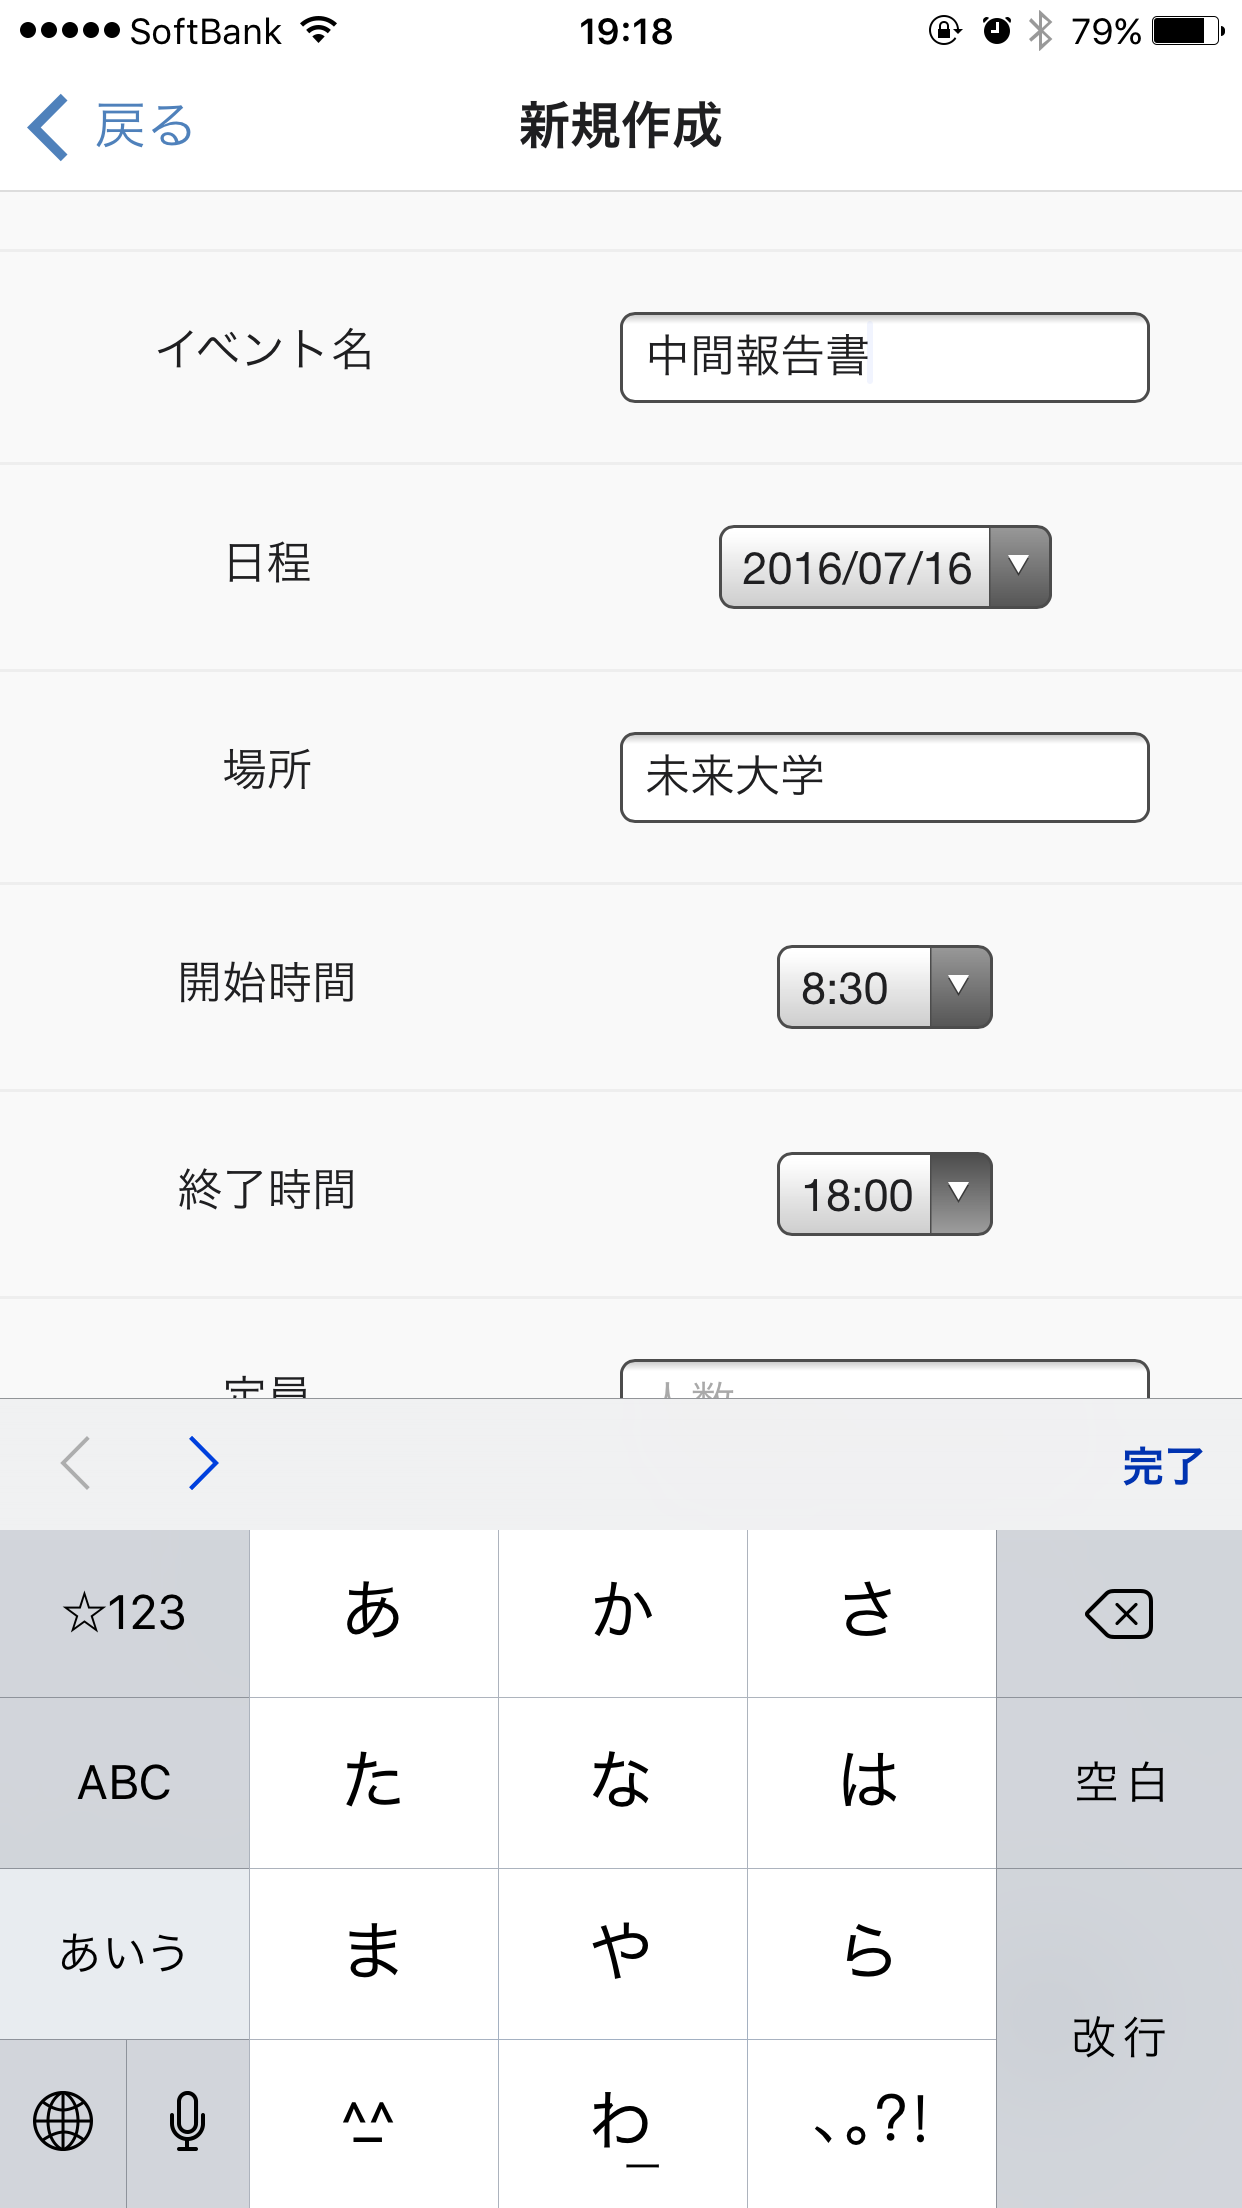
\includegraphics[width=4cm]{event_add.png}}}
          \hspace{1cm}% (b)観光スポットの詳細情報
          {\footnotesize (b)イベント情報の入力画面}
        \end{center}
      \end{minipage}

    \end{tabular}
    \caption{イベント情報の発信}
    \label{tab:trans_event}
  \end{center}
\end{figure}

\subsection{イベント情報の編集機能}%:発表技法について
イベント一覧リスト画面(図\ref{tab:edit_event}(a))から任意のイベントを選択すると, イベント情報の詳細画面(図\ref{tab:edit_event}(b))に遷移する. その後, 右上のメニューボタンからイベントの編集を選択することで, イベント情報の編集画面(図\ref{tab:edit_event}(c))に選択する. イベント情報の編集画面では, イベント情報発信機能と同様に, 11種類の情報を編集した後画面下の更新するボタンを押すことで, イベント情報を再発信することが可能となる. また, イベント詳細画面の右上のメニューボタンから, イベント削除を選択することでイベント情報の削除が可能となる.
\newpage
\begin{figure}[htbp]
  \begin{center}
    \begin{tabular}{c}

      % 1
      \begin{minipage}{0.33\hsize}
        \begin{center}
        {\setlength{\fboxsep}{0cm}\fbox{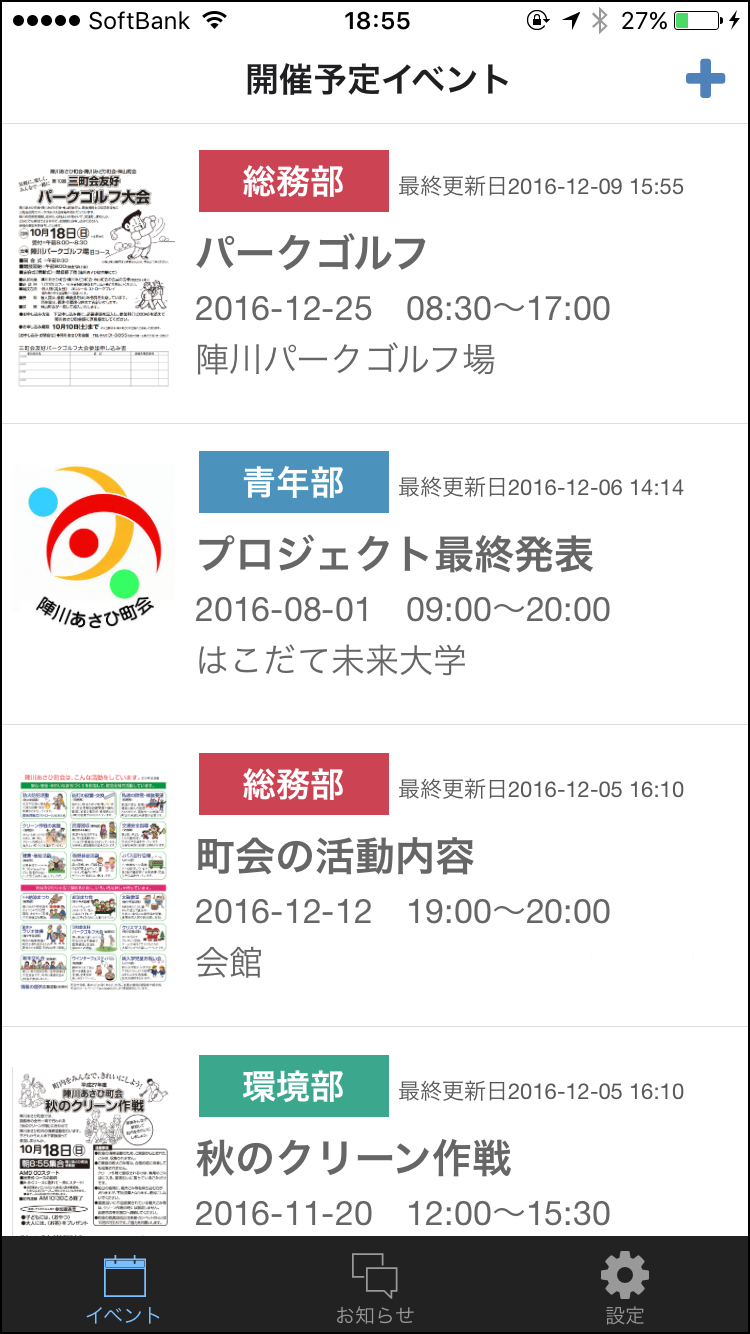
\includegraphics[width=4cm]{event_list.png}}}
          \hspace{1cm} %(a)観光スポットの紹介
          {\footnotesize (a)イベント一覧リスト画面}
        \end{center}
      \end{minipage}

      % 2
      \begin{minipage}{0.33\hsize}
        \begin{center}
        {\setlength{\fboxsep}{0cm}\fbox{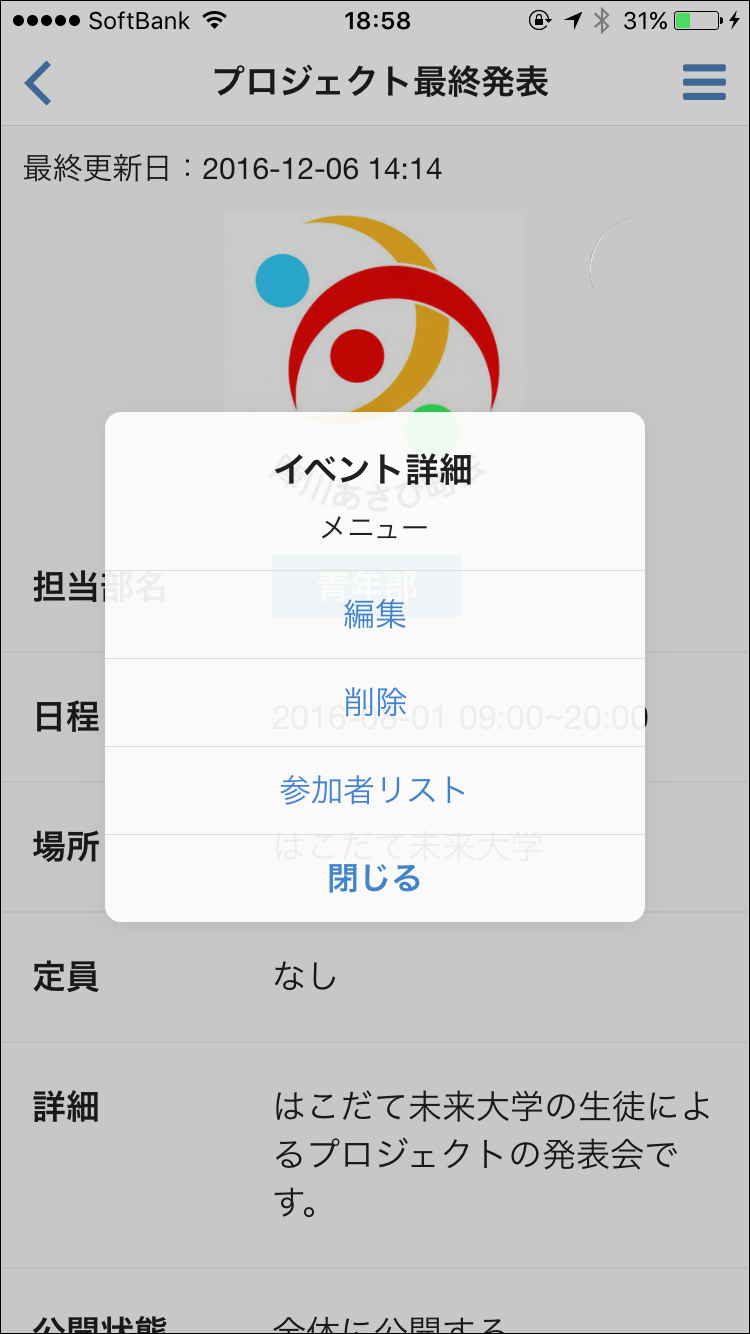
\includegraphics[width=4cm]{event_detail_02.png}}}
          \hspace{1cm}% (b)観光スポットの詳細情報
          {\footnotesize (b)イベント情報の詳細画面}
        \end{center}
      \end{minipage}

      % 3
      \begin{minipage}{0.33\hsize}
        \begin{center}
        {\setlength{\fboxsep}{0cm}\fbox{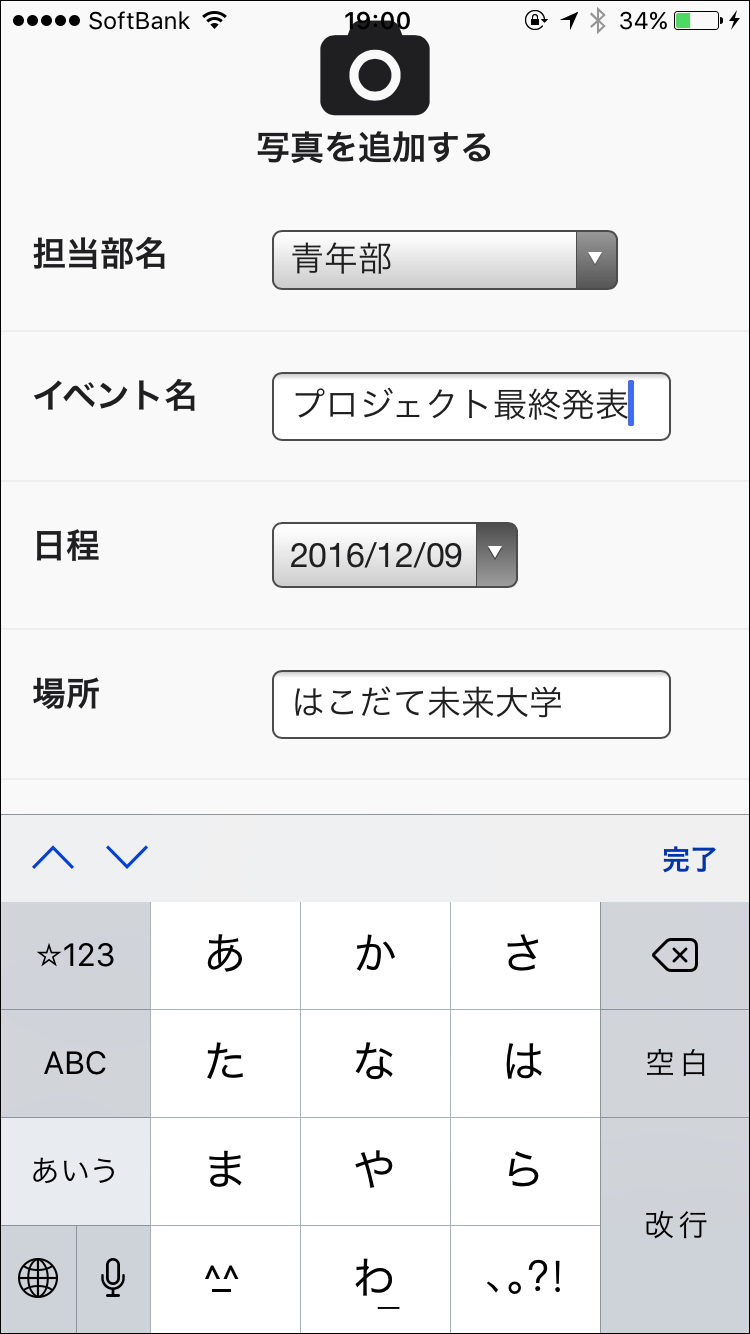
\includegraphics[width=4cm]{event_edit.png}}}
          \hspace{1cm}% (b)観光スポットの詳細情報
          {\footnotesize (c)イベント情報の編集画面}
        \end{center}
      \end{minipage}

    \end{tabular}
    \caption{イベント情報の編集}
    \label{tab:edit_event}
  \end{center}
\end{figure}
\bunseki{横山新}

\section{イベント参加申し込み機能}%例:レビュー内容
\subsection{イベント参加申し込み機能の概要}%:発表技法について
イベント参加申し込み機能とは, 全てのモードで可能な機能であり, イベントへの参加申し込みを行うことを可能とした. 従来は, 町民がイベントへの参加申し込みをする際に, 電話, メール, FAX等多くの方法が存在していため, 町会は参加者の管理に時間を要していた. イベント参加申し込み機能を実装した理由は, この問題を解決し, 町会の負荷を軽減するためである.

\subsection{イベント参加申し込み画面}%:発表技法について
イベント一覧リスト画面(図\ref{tab:event_apply}(a))から任意のイベントを選択すると, イベント情報の詳細画面(図\ref{tab:event_apply}(b))に遷移する. その後, 画面下の参加を申し込むボタンを押すと, イベント参加申し込み画面(図\ref{tab:event_apply}(b))に遷移する. イベント参加申し込み画面では, 入力する情報の属性として氏名, 性別, 年齢, 電話番号, 住所の5つに分けた. これら5つの属性は, ヒアリングを通して定まったものである. このように, 入力する情報の属性を限定していることも, \ref{sec:app_overview}節(\pageref{sec:app_overview}ページ)で記述した「じぷり」が持つ優位性の1つである. 情報を入力した後画面下の確定するボタンを押すことで参加申し込みが可能となる. また, 入力した情報を端末に保存することで, 次回以降の入力を省略することができるようにした。

\begin{figure}[htbp]
  \begin{center}
    \begin{tabular}{c}

      % 1
      \begin{minipage}{0.33\hsize}
        \begin{center}
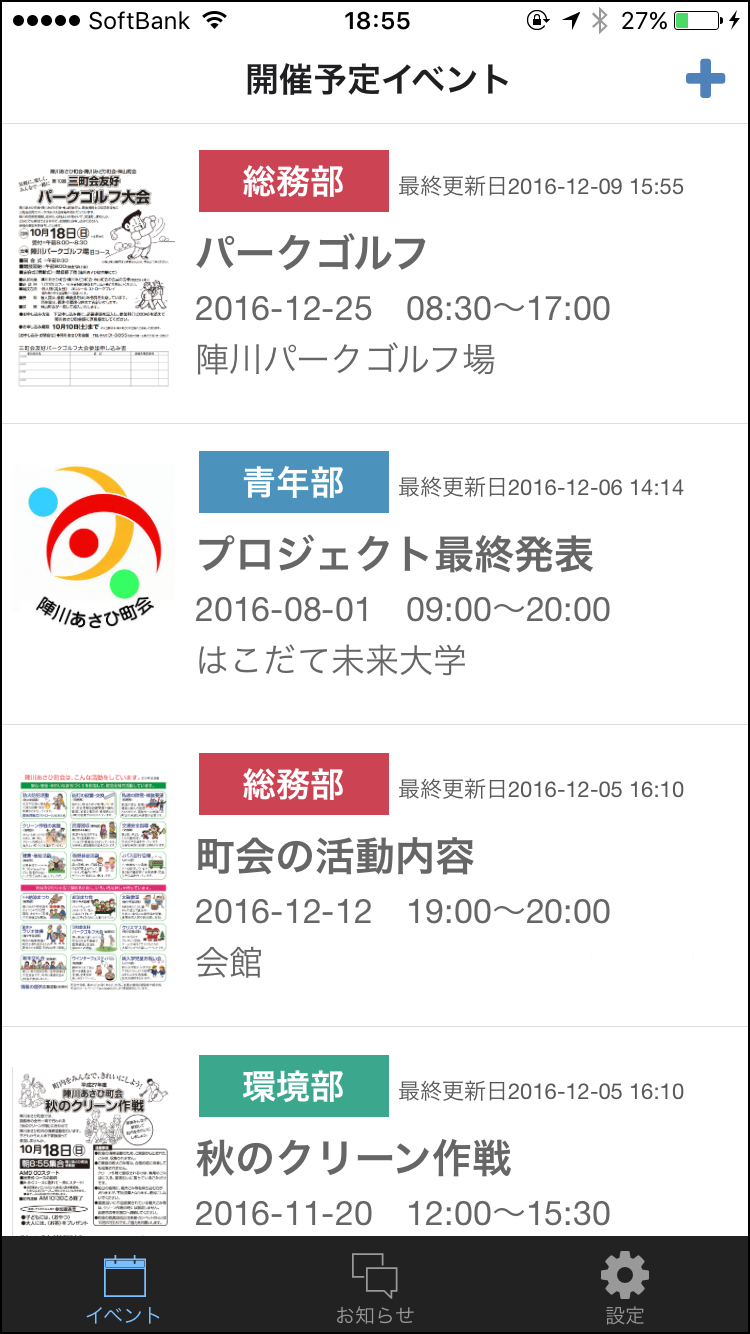
\includegraphics[width=4cm]{event_list.png}
          \hspace{1cm} %(a)観光スポットの紹介
          {\footnotesize (a)イベント一覧リスト画面}
        \end{center}
      \end{minipage}

      % 2
      \begin{minipage}{0.33\hsize}
        \begin{center}
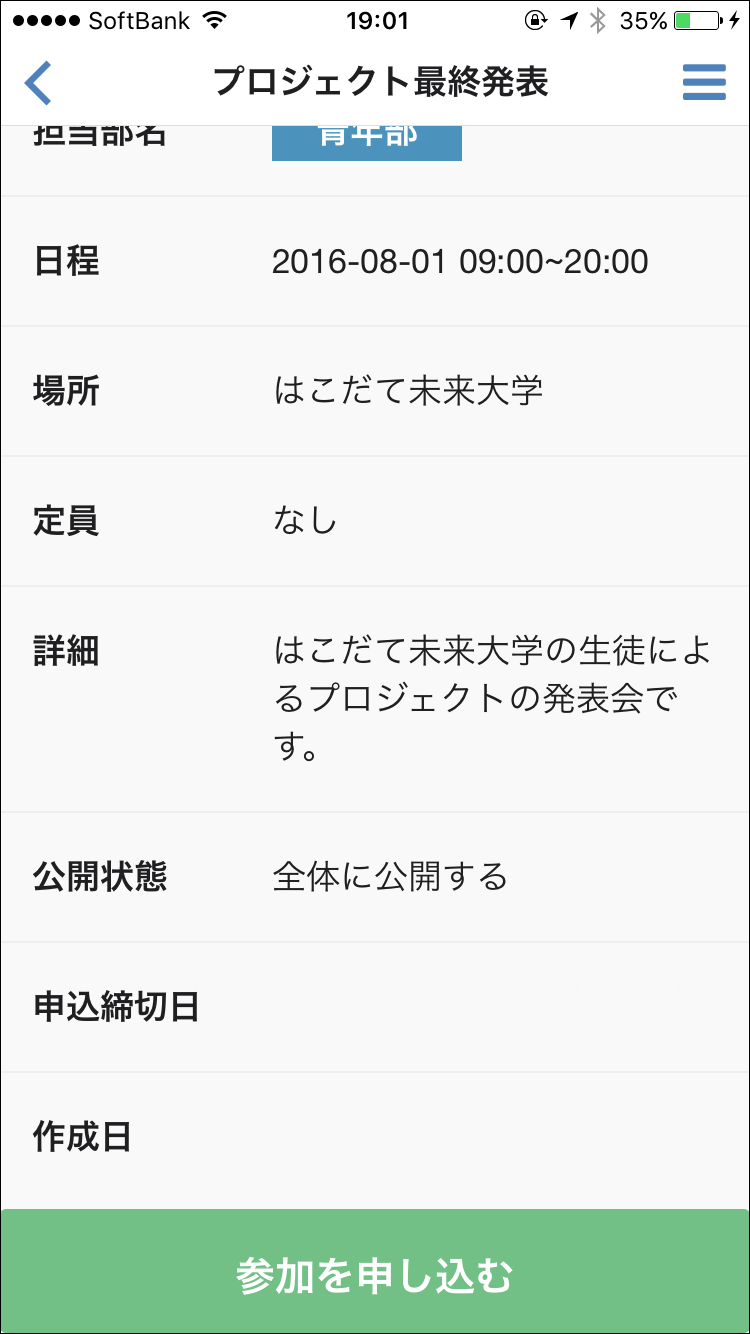
\includegraphics[width=4cm]{event_detail_03.png}
          \hspace{1cm}% (b)観光スポットの詳細情報
          {\footnotesize (b)イベント情報の詳細画面}
        \end{center}
      \end{minipage}

      % 3
      \begin{minipage}{0.33\hsize}
        \begin{center}
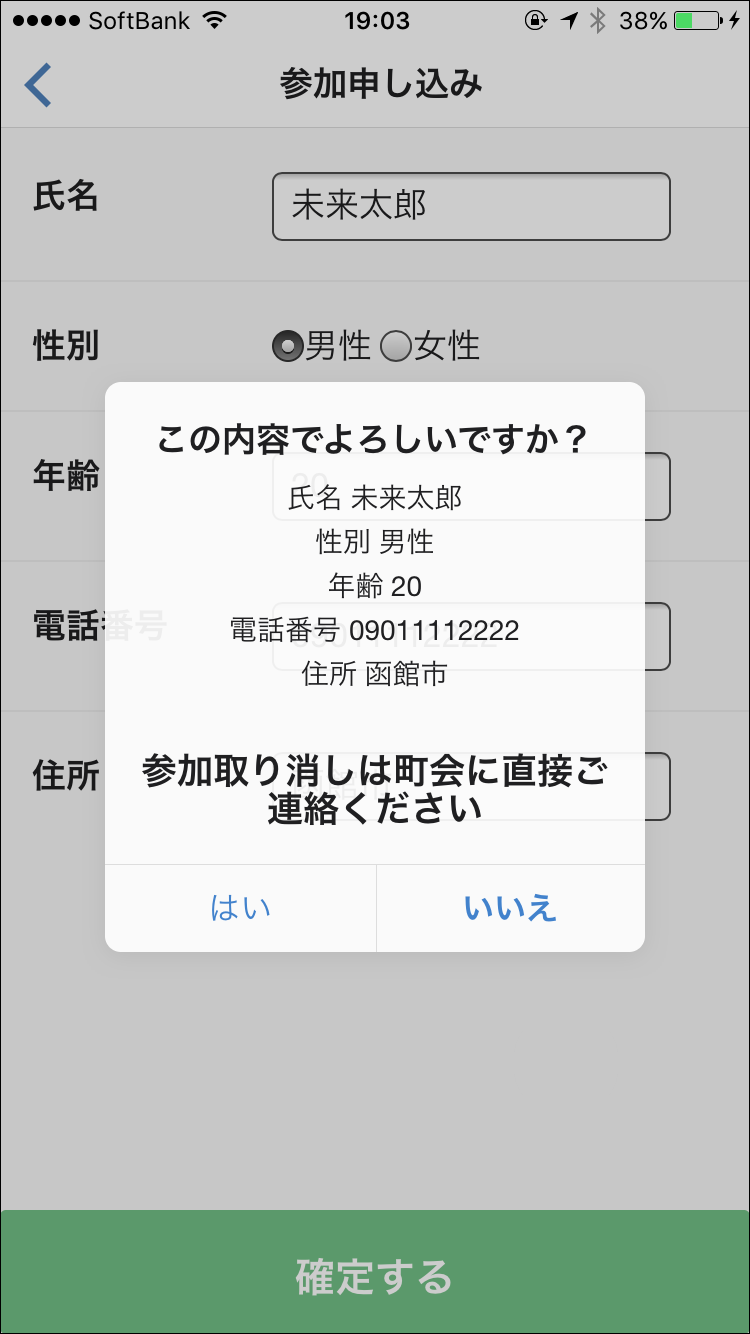
\includegraphics[width=4cm]{participant_form_02.png}
          \hspace{1cm}% (b)観光スポットの詳細情報
          {\footnotesize (c)イベント参加申し込み画面}
        \end{center}
      \end{minipage}

    \end{tabular}
    \caption{イベント参加申し込み}
    \label{tab:event_apply}
  \end{center}
\end{figure}
\bunseki{横山新}

\section{参加者管理機能}%例:レビュー内容
参加者リスト画面は「役員モード」でのみ閲覧可能な画面(図\ref{tab:joinedlist}(a))であり, イベントごとの参加者一覧の表示や参加取り消しを可能としている. また, 右上のメニューボタンから追加参加ボタンを選択すると, 追加参加画面(図\ref{tab:joinedlist}(b))に遷移する. 実装した理由は, 役員がじぷりを使用することができないユーザの代わりに参加申し込みすることや, イベントの申込み締め切り後に役員がユーザから連絡を受け, 代わりに参加参加申し込みを行えるようにするためである. また, 町会へのヒアリングの結果, 参加者リストを市役所に提出する必要があるイベントが存在することがわかった. これを楽に行えるように, 右上のメニューボタンからリスト出力を選択することで, 参加者リストをCSVファイル形式で出力(図\ref{tab:csv})できるようにした. CSVファイルはncmbに保存され, ユーザは画面左上のその他からLINEやGoogleDrive, Dropboxなどに保存(図\ref{tab:joinedlist}(c))することができる. これもまた, \ref{sec:app_overview}節(\pageref{sec:app_overview}ページ)で記述した「じぷり」が持つ優位性の1つである.
\clearpage

\begin{figure}[htbp]
  \begin{center}
    \begin{tabular}{c}

      % 1
      \begin{minipage}{0.33\hsize}
        \begin{center}
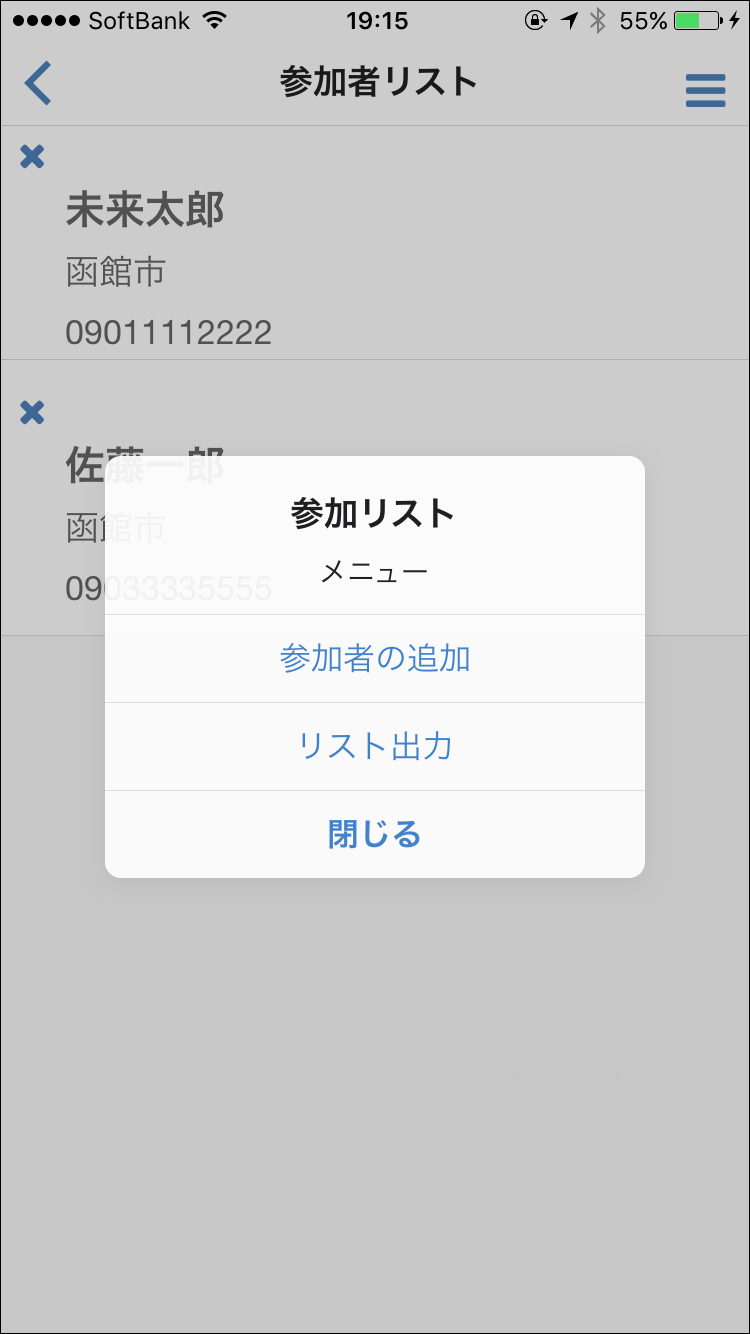
\includegraphics[width=4cm]{participant_list_02.png}
          \hspace{1cm} %(a)観光スポットの紹介
          {\footnotesize (a)参加者リスト画面}
        \end{center}
      \end{minipage}

      % 2
      \begin{minipage}{0.33\hsize}
        \begin{center}
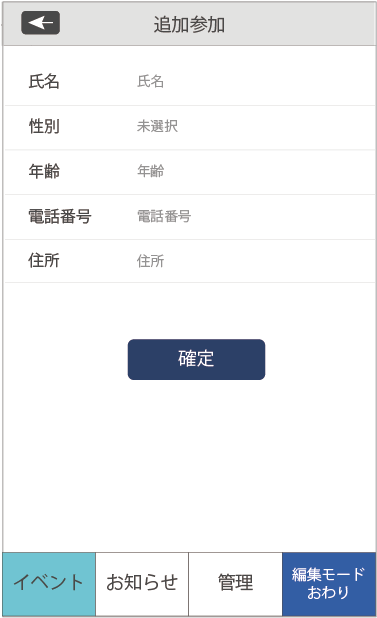
\includegraphics[width=4cm]{participant_add.png}
          \hspace{1cm}% (b)観光スポットの詳細情報
          {\footnotesize (b)追加参加画面}
        \end{center}
      \end{minipage}

      % 3
      \begin{minipage}{0.33\hsize}
        \begin{center}
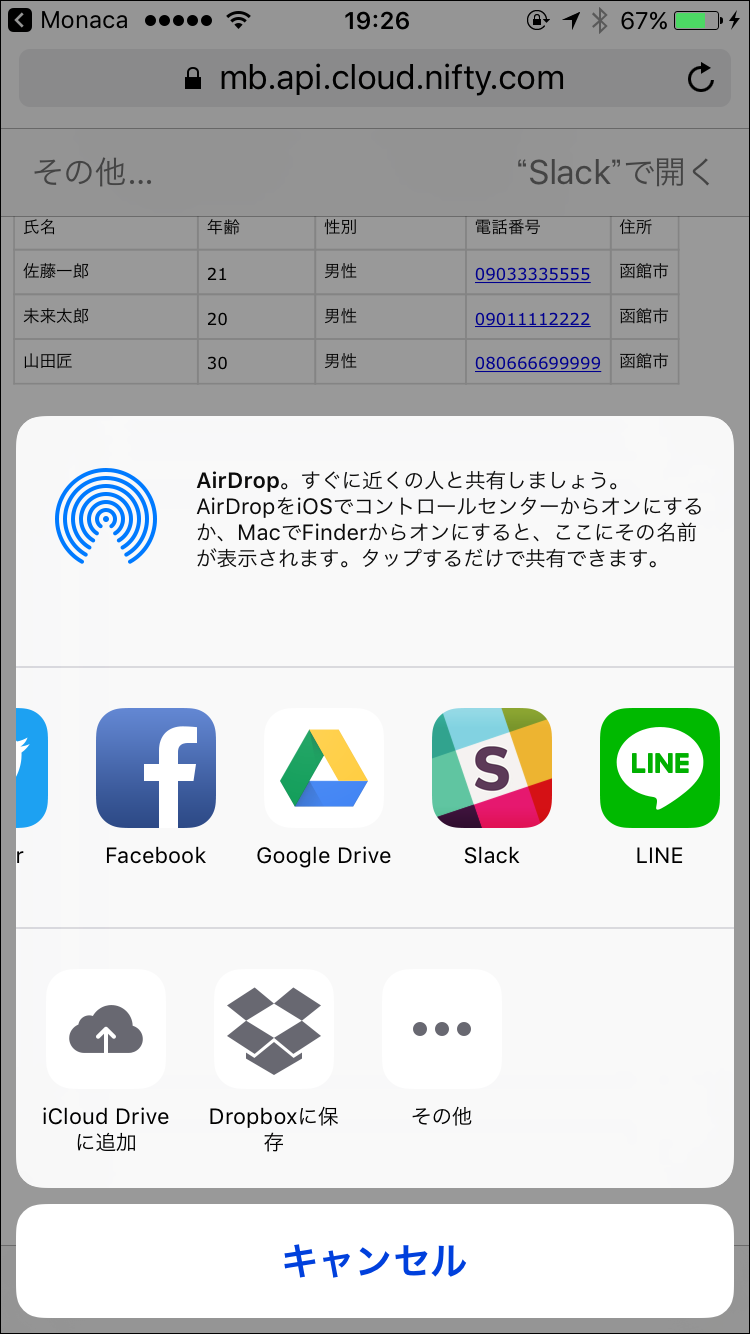
\includegraphics[width=4cm]{participant_list_save.png}
          \hspace{1cm}% (b)観光スポットの詳細情報
          {\footnotesize (c)CSVの保存}
        \end{center}
      \end{minipage}

    \end{tabular}
    \caption{参加者リスト}
    \label{tab:joinedlist}
  \end{center}
\end{figure}

\begin{figure}[htbp]
  \begin{center}
    \begin{tabular}{c}

      % 1
      \begin{minipage}{1\hsize}
        \begin{center}
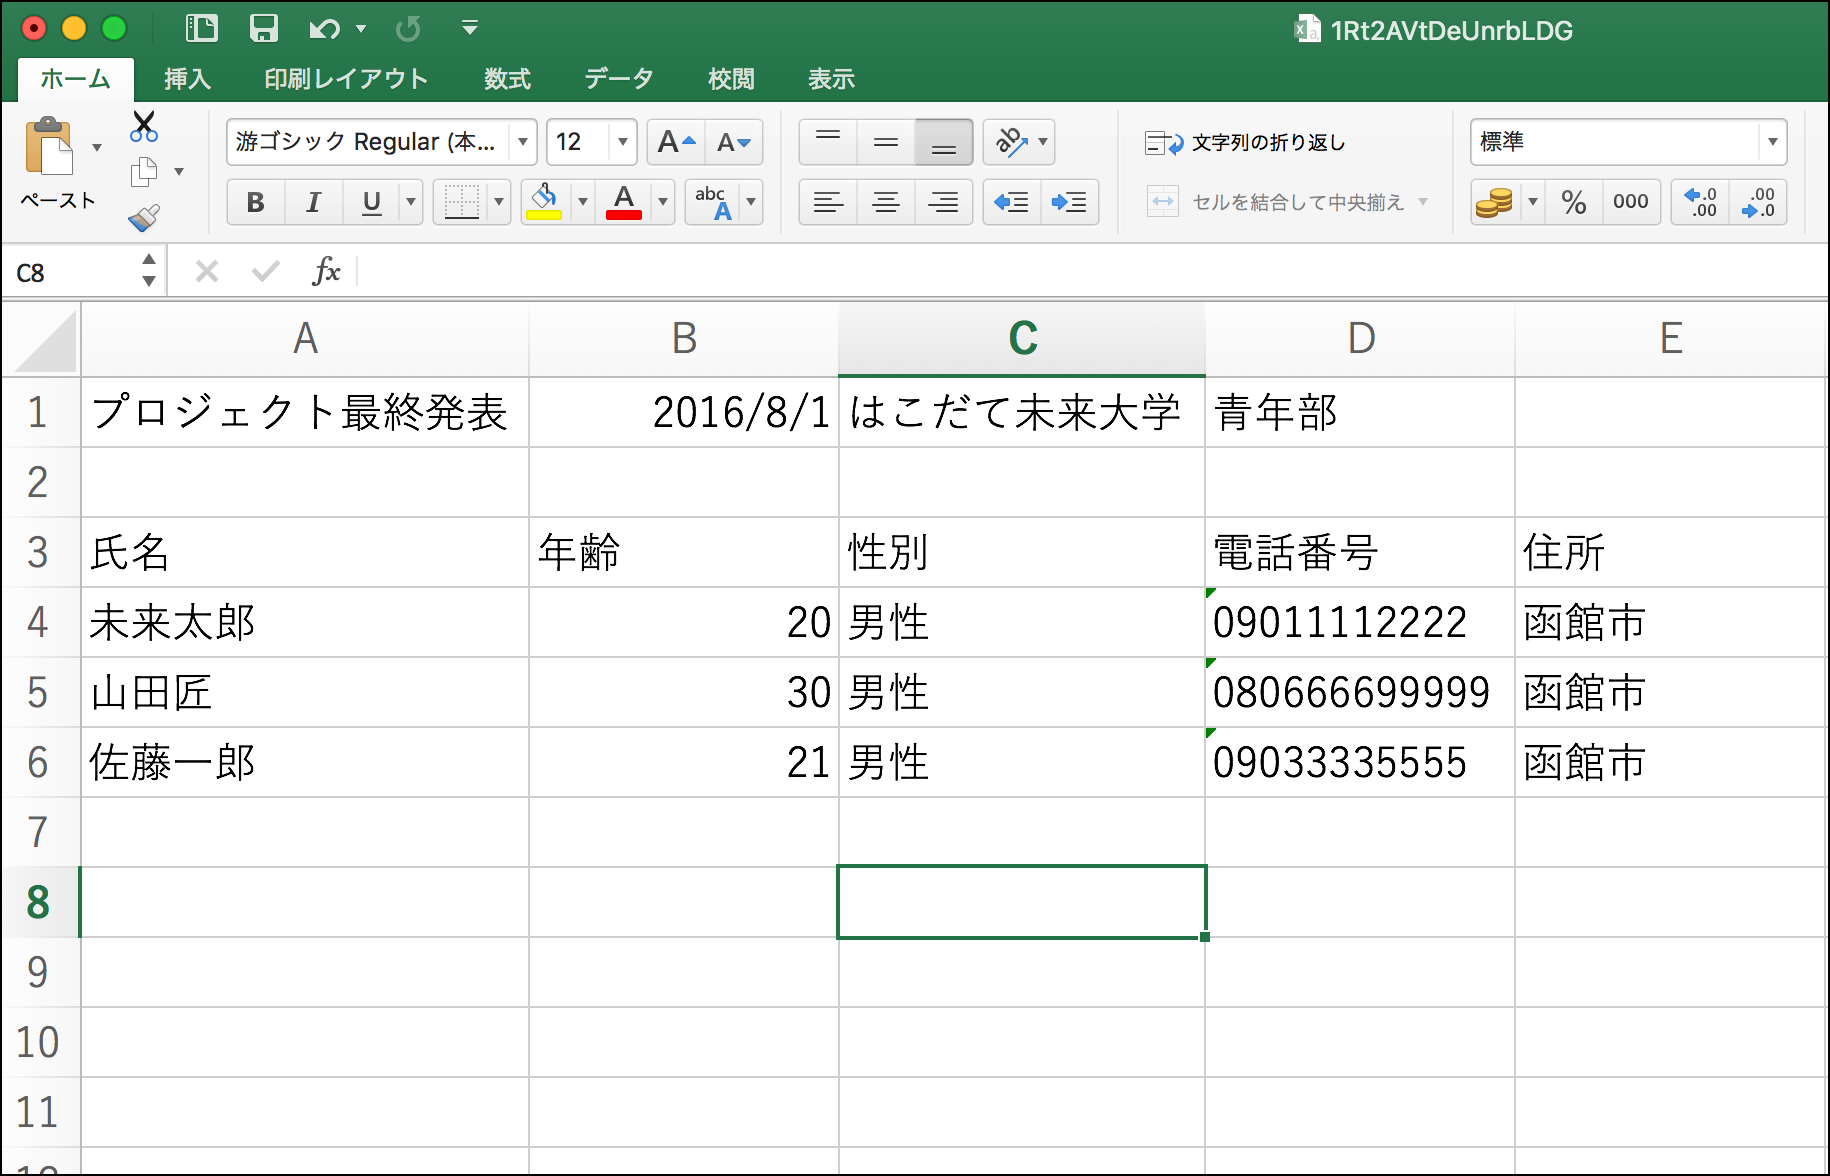
\includegraphics[width=14cm]{csv.png}
          \hspace{1cm} %(a)観光スポットの紹介
        \end{center}
      \end{minipage}

    \end{tabular}
    \caption{出力したCSVファイル}
    \label{tab:csv}
  \end{center}
\end{figure}
\bunseki{横山新}

\section{お知らせ管理機能}%例:レビュー内容
\subsection{お知らせ管理機能の概要}%:発表技法について
お知らせ管理機能とは「役員モード」での利用可能な機能であり, 町会からのお知らせを発信, 発信したお知らせの削除を可能とした. これらは, 管理者のみが使うことを可能とした. お知らせ機能を実装した理由は, \ref{problems}節でも記述したが過去のイベントで雨天中止の連絡ができなかったために, 参加者に風邪を引かせてしまったという事例があったことから, 町会からのお知らせを迅速に参加者に伝える必要があると判断したからである. またこの機能を用いて, 「今日は燃えるゴミが出せる日」「午後から雨が振るので, 洗濯物は取り込んでおいて下さい」といった生活情報の発信も行うことが可能となる.


\subsection{お知らせ作成画面}%:発表技法について
お知らせ一覧リスト画面(図\ref{tab:trans_info}(a))からプラスの形をしたボタンを押すと, お知らせの新規作成画面(図\ref{tab:trans_info}(b))に遷移する. お知らせの新規作成画面では, 担当部名, タイトル, お知らせ内容を入力し役員のみに公開するか否かを選択した後画面下の作成するボタンを押すことでお知らせを発信することが可能となる. 担当部名については, 第\ref{subsec:event_add}項(\pageref{subsec:event_add}ページ)で記述したイベント情報の発信機能と同様に担当部ごとに色を付けた.

\begin{figure}[htbp]
  \begin{center}
    \begin{tabular}{c}

      % 1
      \begin{minipage}{0.33\hsize}
        \begin{center}
        {\setlength{\fboxsep}{0cm}\fbox{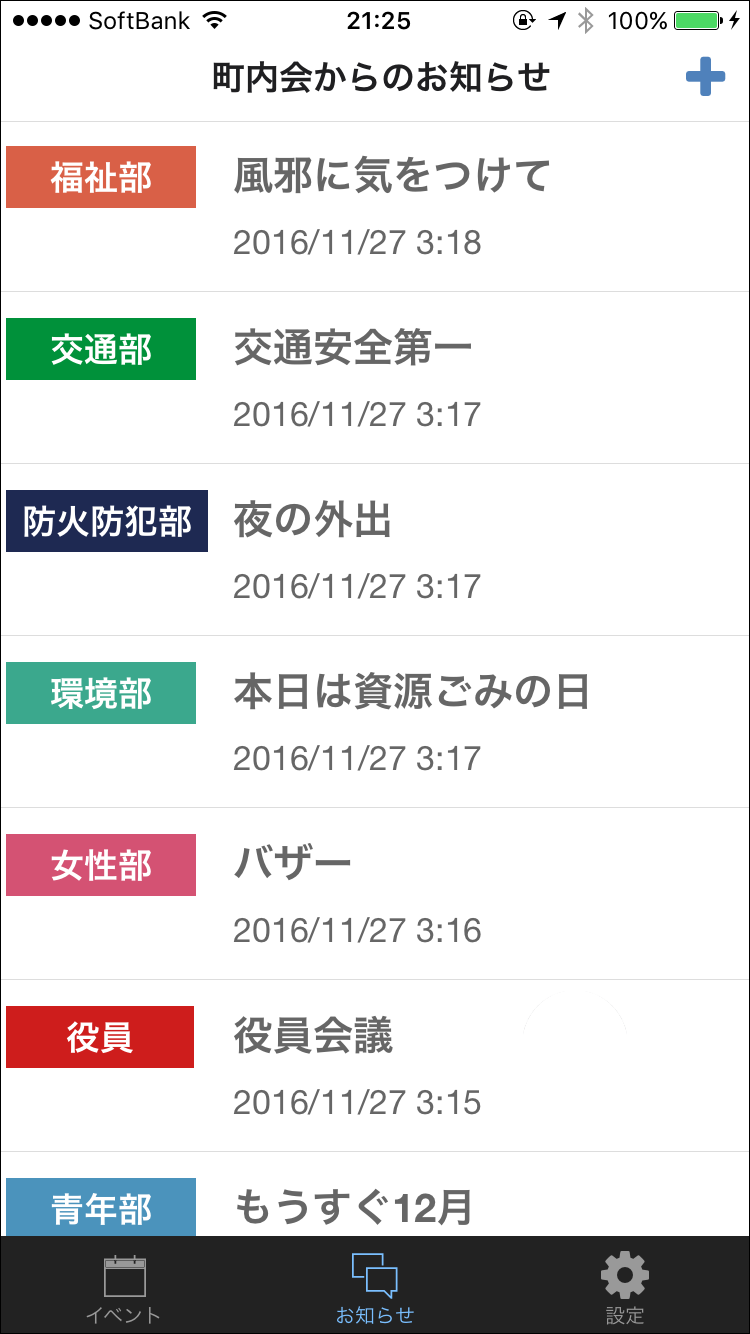
\includegraphics[width=4cm]{information_list_01.png}}}
          \hspace{1cm} %(a)観光スポットの紹介
          {\footnotesize (a)お知らせ一覧リスト画面}
        \end{center}
      \end{minipage}

      % 2
      \begin{minipage}{0.33\hsize}
        \begin{center}
         {\setlength{\fboxsep}{0cm}\fbox{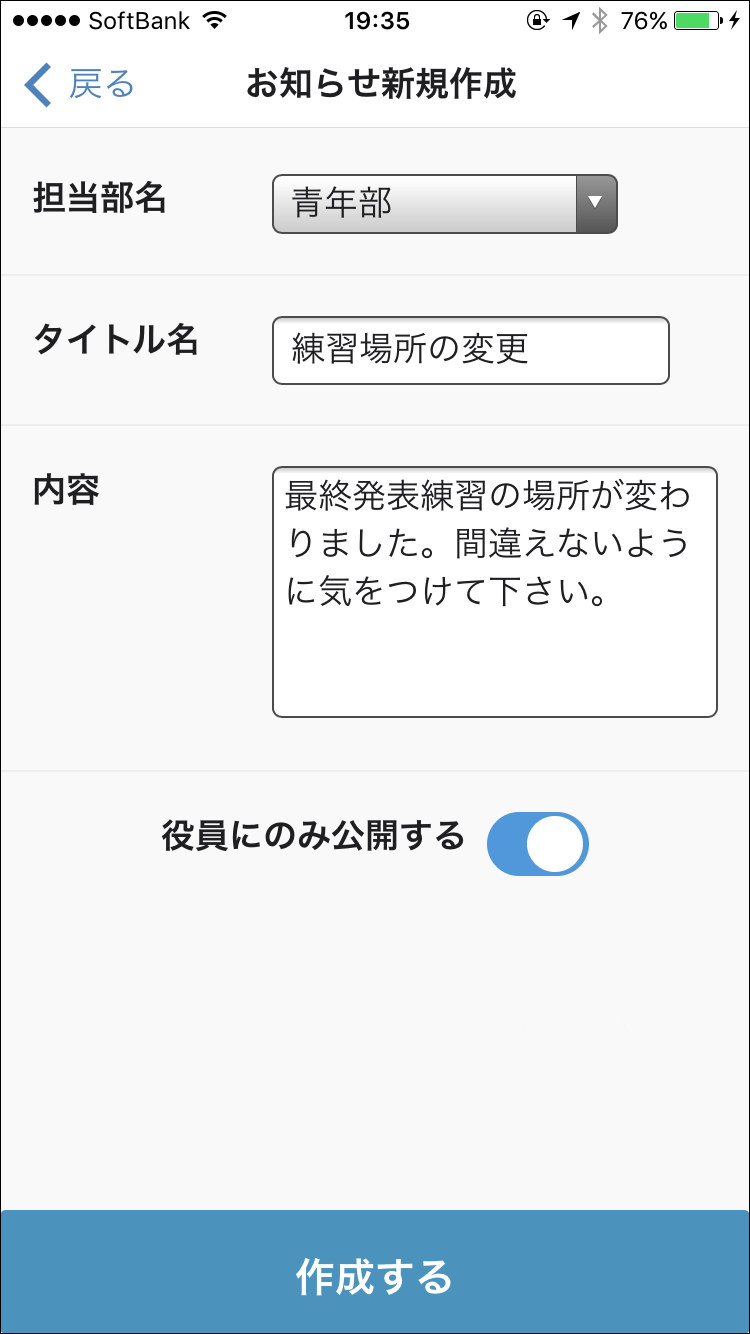
\includegraphics[width=4cm]{information_add.png}}}
          \hspace{1cm}% (b)観光スポットの詳細情報
          {\footnotesize (b)お知らせの新規作成画面}
        \end{center}
      \end{minipage}

    \end{tabular}
    \caption{お知らせ作成}
    \label{tab:trans_info}
  \end{center}
\end{figure}
\newpage
\subsection{お知らせ削除}%:発表技法について
お知らせ一覧リスト画面(図\ref{fig:delete_info})から削除したいお知らせを選択した後, 削除ボタンを選択して, 発信したお知らせの削除を行う.

\begin{figure}[htbp]
  \begin{center}
    \begin{tabular}{c}

      % 1
      \begin{minipage}{0.33\hsize}
        \begin{center}
        {\setlength{\fboxsep}{0cm}\fbox{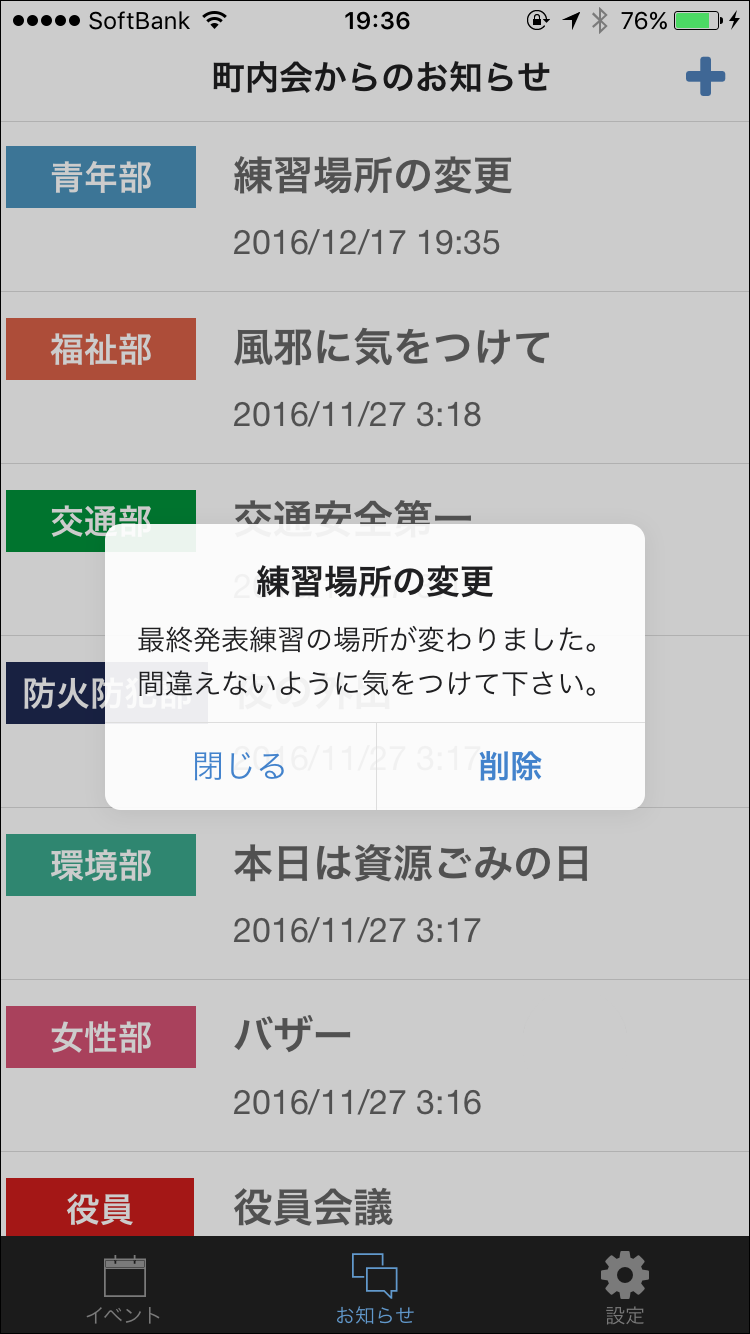
\includegraphics[width=4cm]{information_list_02.png}}}
          \hspace{1cm} %(a)観光スポットの紹介
        \end{center}
      \end{minipage}

    \end{tabular}
    \caption{お知らせの削除}
    \label{fig:delete_info}
  \end{center}
\end{figure}
\bunseki{横山新}


%中間発表
\chapter{中間発表}
​
\section{発表形式}
7月8日に行われた中間発表では、各グループが行ってきた活動を詳細に伝え、後期の活動に活かせるレビューをもらうことを目的とした。
そのため全体ポスター2分、各グループのポスターとデモを含めた発表を12分間並行して発表を行った。
\bunseki{伊藤泰斗}

\section{レビュー内容}%例:レビュー内容
%必要なら下のsubsectionを用いて小見出しをつかう
\subsection{発表方法についての評価と反省}%:発表技法について
以下に、中間発表会で行ったアンケートの「発表技術について」の項目から、メンバ間で精査した結果、最終成果発表にも取り入れたいコメントを抜粋した。
\begin{itemize}
  \item デモがプロトタイプであることを伝えないと、実装したものだと勘違いしてしまう。
  \item もう少しスラスラ話せていたら分かりやすかったと感じた。
\end{itemize}
    上記より、伝える情報とポスターセッションの練習の不足が伺える。
    しかし、「とても喋りに安定感があるなと感じた」との評価も受けた。最終成果発表の際にはすべて開発したアプリケーションでデモを行い、
    ポスターセッションをする人全員がスラスラと話せるくらいに練習を行っていく。

\subsection{発表内容についての評価と反省}
    「発表内容について」の項目から後期の開発や発表において考慮すべきコメントを抜粋した。
\begin{itemize}
  \item 陣川町民に使ってもらうためのプロモーションの方法を考えたほうが良い
  \item クーポンなど、ユーザを得る工夫が欲しい
  \item ユーザにより沿って開発していく中で生起した出来事を大切に記述して欲しい
\end{itemize}
    上記より、2つの見落としが伺えた。1つ目はユーザに使ってもらうための考慮をしていなかったことである。
    メンバ全員が使ってもらえることを前提として考えていることである。しかし実際には使ってもらえることは前提ではないため、
    どのようにして使ってもらうのかを考える必要がある。2つ目は、本アプリケーションにユーザにとって魅力的な優位性が必要であることである。
    認知されていてもユーザにとって使いたいものでなければ使ってもらうことができない。そのため、最終成果発表までにプロモーションの方法を考え、
    使ってもらうための工夫を本アプリケーションに追加することでユーザを獲得していきたい。
\bunseki{伊藤泰斗}


%前期のプロジェクト振り返り
%\chapter{振り返り}
我々は7月13日にこれまでの活動の振り返りを行った。
はじめに、5月から我々が行ってきたこと、その際に感じたこと、
心に残ったアドバイスについてそれぞれ黄色、緑、赤の付箋に書き出した。
その後、それらを2枚の模造紙に期間ごとに貼り付けてグループメンバー全員で見返した。
その次に、我々は今までの活動の中で良い点、悪い点、これからやっていきたいことを話し合った。
良い点として、メンバー間で積極的にコミュニケーションを取り合うことでメンバーの関係性を良好に保てたことが挙げられた。
悪い点として、メンバーの予定を考慮することなくスケジュールの決定を行った点、各作業に要する時間の想定が困難だったため、メンバーに負担がかなり掛かってしまった点が挙げられた。
これからやっていきたいこととしては、TAや教員等相談できる人がいるという環境を有効に活用することで、活動が行き詰まり遅れる時間を削減していきたいということが挙げられた。
我々はこの振り返りを通して5月からの活動を客観的に見ることができた。上記の気づきを、後期の活動にしっかりと活かしていきたい。


%今後の展望
\chapter{今後の展望}

\section{不具合を解消}
11月18日の町会打ち合わせにて役員に開発途中のじぷりを利用してもらったところ, iOS,  Android共に動作が不安定であることがわかった.
iOSでは, イベントの新規作成をすることができるが, イベントの更新をすることができなかった. Androidでは, イベントの新規作成時に写真の追加をすることができなかった.
今後, それぞれの原因を特定して解消していく. 解消後は1月11日~20日の町会打ち合わせにじぷりを実際に利用してもらい, そこで出た要望や問題を解決し最終調整を行い, 1月31日までにリリースする予定である.
\bunseki{船木綾香}

\section{無償サーバサービスの利用}
現在, 無償サーバサービスのmBaaSを利用している. 町会の意向により今後も無償のサービスを利用していく. しかし, じぷりのサーバへのリクエスト回数が無料の範囲を超えてしまう場合は,
無償のサーバサービスでは運用することが難しいため町会で独自のサーバを立ち上げる可能性がある.
\bunseki{船木綾香}

\section{機能の追加と改善}
私たちは, 陣川町民の多くの人にじぷりを長く利用してもらいたいと考えている. そのため, 今後は今期に実装できなかった機能を追加していく予定である. 具体的な機能を以下に示す.
\begin{itemize}
    \item イベントへの参加申し込みが来た時にイベント管理者へ通知が行われる機能
    \item 特定のイベントの参加者のみにメッセージを送る機能, イベントへの参加者自身で参加の申し込みを取り消す機能
    \item イベント参加者がイベントへの参加を取り消した場合, イベント管理者へ通知が行われる機能
    \item イベント開催する担当部署ごとに通知のオンオフを切り替える機能
    \item イベントが新しく追加された時にじぷりを持っている全ユーザへ通知がされる機能
    \item 自分が参加する予定のイベントを確認できる機能
\end{itemize}
また, 現在のじぷりはスマートフォンの操作に慣れていない人でも利用しやすいUIを目指して作っているが,
今後は幅広い年齢層の方や町民外の方にでも利用してもらえるようなUIに改善していく予定である.
\bunseki{船木綾香}


%前期の振り返りと学び
\chapter{振り返り}

\section{前期の振り返り}
7月13日にプロジェクト学習前期活動の振り返りを行った. はじめに, 5月から我々が行ってきたこと, その際に感じたこと, 心に残ったアドバイスについてそれぞれ黄色,緑,赤の付箋に書き出した.その後,
それらを2枚の模造紙に期間ごとに貼り付けてグループメンバ全員で見返した.その次に,我々は今までの活動の中で良い点,悪い点,これからやっていきたいことを話し合った.
良い点として,メンバ間で積極的にコミュニケーションを取り合うことでメンバの関係性を良好に保てたことが挙げられた.悪い点として,メンバの予定を考慮することなくスケジュールの決定を行った点,
各作業に要する時間の想定が困難だったため,メンバに負担がかなり掛かってしまった点が挙げられた.これからやっていきたいこととしては, TAや教員等相談できる人がいるという環境を有効に活用することで,
活動の行き詰まる時間を削減することが挙げられた.我々はこの振り返りを通して5月からの活動を客観的に見ることができた.
\bunseki{森島帆南}

\section{後期の振り返り}
12月21日に前期と後期を含めたプロジェクト活動全体で起きたことを深く掘り下げるために振り返りを行った. はじめに, 前期のKPTを小さい模造紙にまとめた.
次に, 後期のマイルストーンごとに, チームや個人で取り組んだこと, その時に思っていたこと, その要因をそれぞれ緑, 黄色, 赤の付箋に書き出し, 別の模造紙に貼り付けた.
その後, メンバで貼り付けた情報を共有し, これまでの活動の良かった点, 悪かった点について話し合った. 良い点として,
\begin{enumerate}
    \item Trelloを用いて, スプリントバックログとプロダクトバックログの作成・管理を行ったこと
    \item 町会打ち合わせで議事録ドリブンを導入したことの2点が挙げられた.
\end{enumerate}
Trelloを利用した理由は, タスクの移動が容易であり操作がしやすいことやRedmineは学外からのアクセスができないからである.
Trelloを使い始めてから, 残りのタスクの数が可視化されて全体の進捗が把握しやすくなり, タスクの管理の効率が良くなった. 議事録ドリブンを導入した理由は, 町会打ち合わせで要望がたくさん出てしまい,
まとめるのが大変であったためである. 議事録ドリブンを導入したことで, その場で要望を整理し, 役員の方たちと共有しながら確認することができ, 普段より要望の整理にかかる時間を短縮することができた.
以上の2点がメンバ全員が後期の活動の中で特に良かったと感じることであった. また, メンバの1人からは, 自身で開発しているため, 操作性についてまったく気にしていなかったが,
実際に先方に使ってもらった時に操作に手間がかかっていた部分があることが発覚し, 改めてUIの大切さを身をもって感じたという意見があった.
悪い点として, 計画的なスケジュールを組み立てられなかったことが1番の反省点に挙げられた. スケジュールを立てる際に, 自分たちの実力が不明だったのでタスクの期日を定めることができなかった.
しかし, 最終的な目標を立ててしっかりとした期日を設けて, それまでにタスクを終わらせる方針をとっていれば, スケジュールが詰まらずに余裕をもって活動を行えたと考えられる.
\bunseki{森島帆南}

\chapter{学び}
\section{先方との打ち合わせ}
先方と行ってきた打ち合わせに関しての3つの問題があった.
1つ目は十分に打ち合わせの事前準備が行えていなかったことである. 事前に打ち合わせの目的を明確にして, 先方に必ず確認すべきことを定めておくことの重要性を学んだ.
また, 先方に見せる資料のピアレビューを必ず全員で行うことも大切であると学んだ. 実際に, メンバの1人が作成した資料を確認しておらず, 打ち合わせ直前に確認したところ, 説明不十分の部分があり,
資料訂正に時間を割かれてしまい, 打ち合わせの練習ができないことがあった. 事前に全員が資料に目を通していれば, 余裕を持ってより先方にとって理解しやすい資料を作成できる可能性があった.

2つ目は, 打ち合わせの進め方の効率が悪いことである. 打ち合わせ中に先方から要望が数多く出てしまいまとめるのが大変であった. この問題から, 打ち合わせを進行しながら議事録を書いていく議事録ドリブンを導入した.
議事録ドリブンを導入したことで, 要望を整理することができる. また, 打ち合わせの最後に先方の方を含め全員で打ち合わせの内容を振り返ることが簡単にできるようになり, 打ち合わせの時間も短縮することができた.

3つ目は, 先方の要望の分析が不足していたことである.
前期では, 先方からの数多くの要望をメンバ全員ではなく, 各々で重要な部分をまとめようとしてしまった. 先方の要望の本質の分析不足で先方にとって本当に使いやすいとは言えないものを提案してしまった.
教員からも先方にとって満足のできるものになっているのか見直した方が良いとのレビューを受けた. 我々はもう1度先方の要望を洗い出し, 先方の本当に求めているものを別のアプローチから解決できないか分析し直した.
また, 全ての機能を書き出した後にそれぞれの優先順位をつけることで, 機能が可視化されて同時に進行した方が作業の効率が良くなる機能なども確認することができた.
\bunseki{森島帆南}
\section{メンバ間の情報共有}
チーム全体でのメンバ間の情報共有に関して, 2つの問題が起きてしまった.
1つ目は, チーム全員での議論時に個人個人の認識に差異が生じてしまうことがあった. メンバ全員が個人のパソコンに向かって話している状態になっていることが多くあり,
同じ認識を持っているかを確認しないまま話を進めてしまったからである. 改善策としてスクリーンを用いての画面共有と席替えを行った. スクリーンを用いて,議論の進行に必要な画面を投影することで,
全員が同じ認識で議論を進めることができた.また,席替えではリーダーが真ん中に座りメンバ全員に質問を振りながら議論を進めることで,メンバ間の認識に差異が生まれにくくすることができた.

2つ目は, チーム全体のタスクの進捗が把握できていなかったことであった. 前期では, メンバ個人個人の忙しさと期日を考慮せずにタスクを割り振ってしまい進捗に偏りが出てしまった.
この反省点から, チーム全体のタスクの進捗が把握できていなかったことであったとわかった. 後期から, スプリントバッグログとプロダクトバッグログをTrelloで管理し始め,
プロジェクト全体のタスクが可視化されてお互いの役割を把握しやすくし進捗が遅れているメンバのサポートをしやすくなった.
\bunseki{森島帆南}

\section{システムコースとデザインコースの考え方の違い}
本チームは情報システムコース1名と情報デザインコース2名と高度ICTコース2名で構成されていたため, 2つの問題が起きてしまった.
1つ目は, チーム全体のコミュニケーションが不足してしまったことであった. システム班とデザイン班に分かれて活動するようになり, チーム全体でのコミュニケーションを取る時間が減ってしまった.
結果, わからないことを確認する機会がなくわからないことや疑問におもっていることをそのままにしてしまっていた. そこで我々は, プロジェクト活動の最初に前回までのタスクの進捗報告をすることを始め,
全体でのコミュニケーションをとりやすくすることでタスクでのわからないことを共有し解決することができた.

2つ目は, システム班とデザイン班の意思疎通がうまく噛み合わないことであった.
デザイン班がじぷりの仕様が大きく変わる案を考え, システム班に変更内容を伝え承諾を得た. しかし, しばらく経った後に仕様の変更内容がシステム班に正しく伝わっていないことがわかり,
説明し直さなければいけないことがあった. お互い得意とする分野が違い専門的な知識や考え方が大きく異なるためデザインの感覚の言葉選びではなく,
システム班の人たちが理解しやすいように仕様変更内容の理由を伝えるべきであった. こうすることで, 専門的な知識が異なってもお互いの意思疎通ができることを学んだ.
\bunseki{森島帆南}

\section{スケジュール管理}
前期, 後期を通してスケジューリングの粗さが目立った. 自分たちの実力や, 忙しさを考慮せずにスケジュールを立てた結果リスケジューリングを余儀なくされる場面が多く見られた. さらに, リスケジューリングする際の各タスクの工期の見積もりが甘く, リスケジューリングを繰り返す場面も多く見られた. また, リスケジューリングした後に町会との打ち合わせが企画されたり, 仕様の変更などが要求された結果スケジュールが大きく乱れた場面も見られた.
これらの経験からスケジュールを立てる時は, 各タスクに対して余裕を持って工期をを見積もることと, リスケジューリングをする際は今あるタスクへの影響度などを考慮した上で, リスケジューリングすべきだということを学んだ. また, 作業に必要な時間, 担当者, 作業の洗い出し, 期限を設定しいつでも確認できるようにすることで, 忘れることなく作業に取り組むことができた.
\bunseki{森島帆南}


% 以降、付録(付属資料)であることを示す
\begin{appendix}

\chapter{5月30日提案資料}
\begin{figure}[ht]
    \begin{center}
      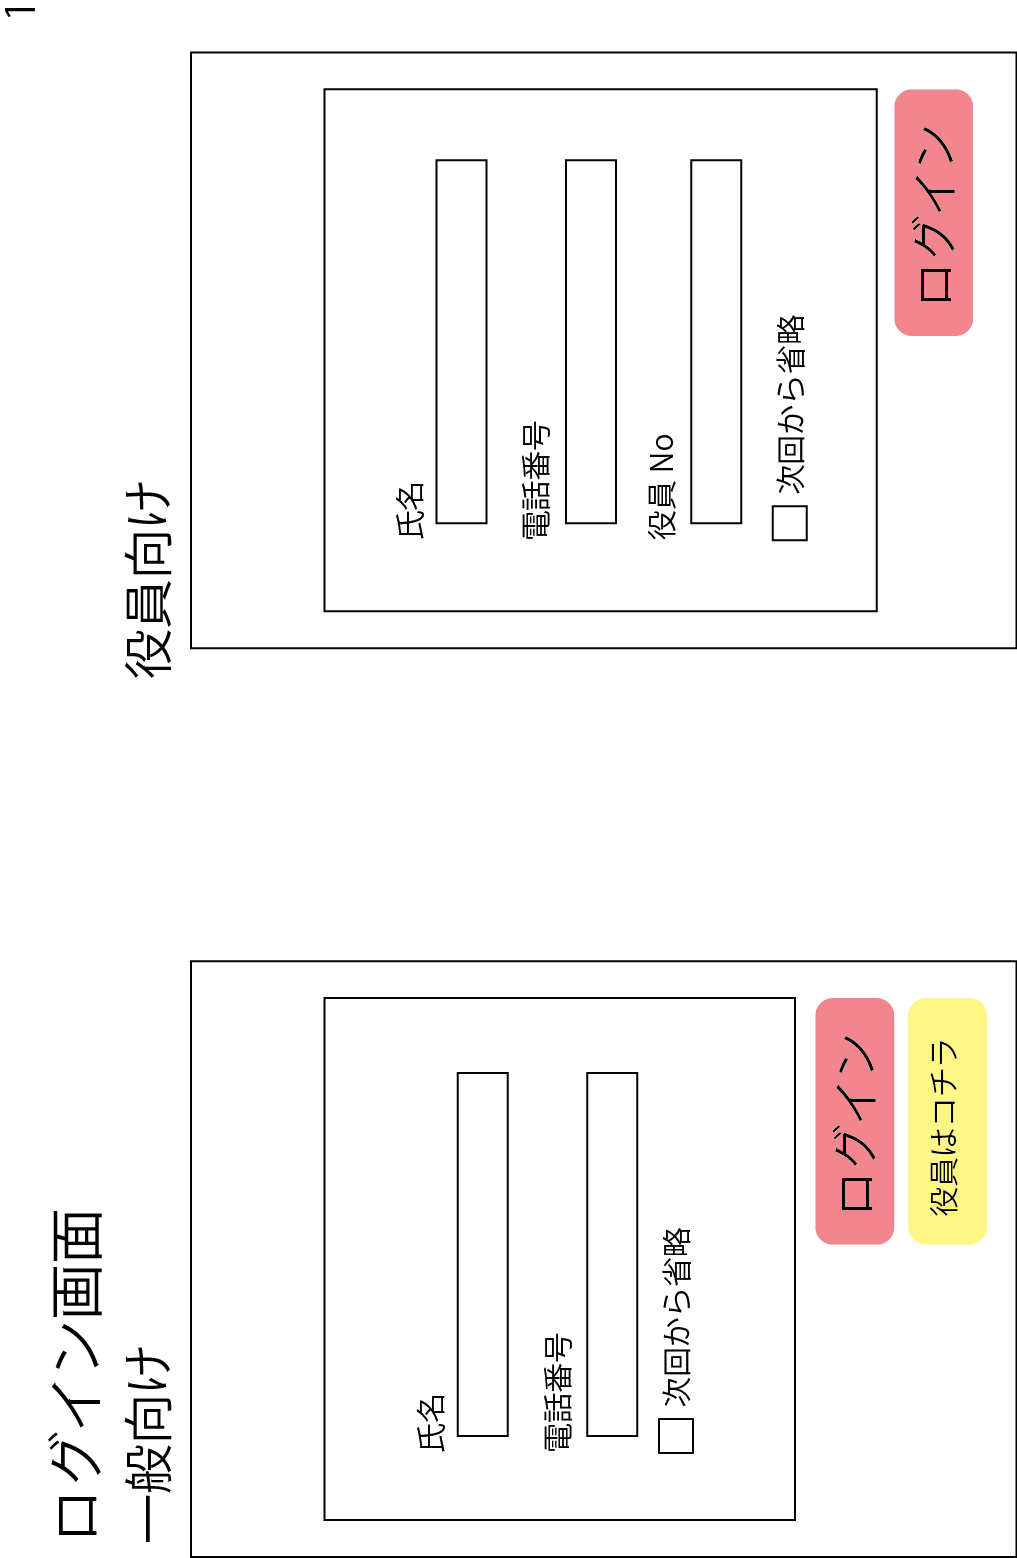
\includegraphics[keepaspectratio, scale=0.7]{appendixs/appendixA_figres/fig1.png}
    \end{center}
\end{figure}

\begin{figure}[ht]
    \begin{center}
    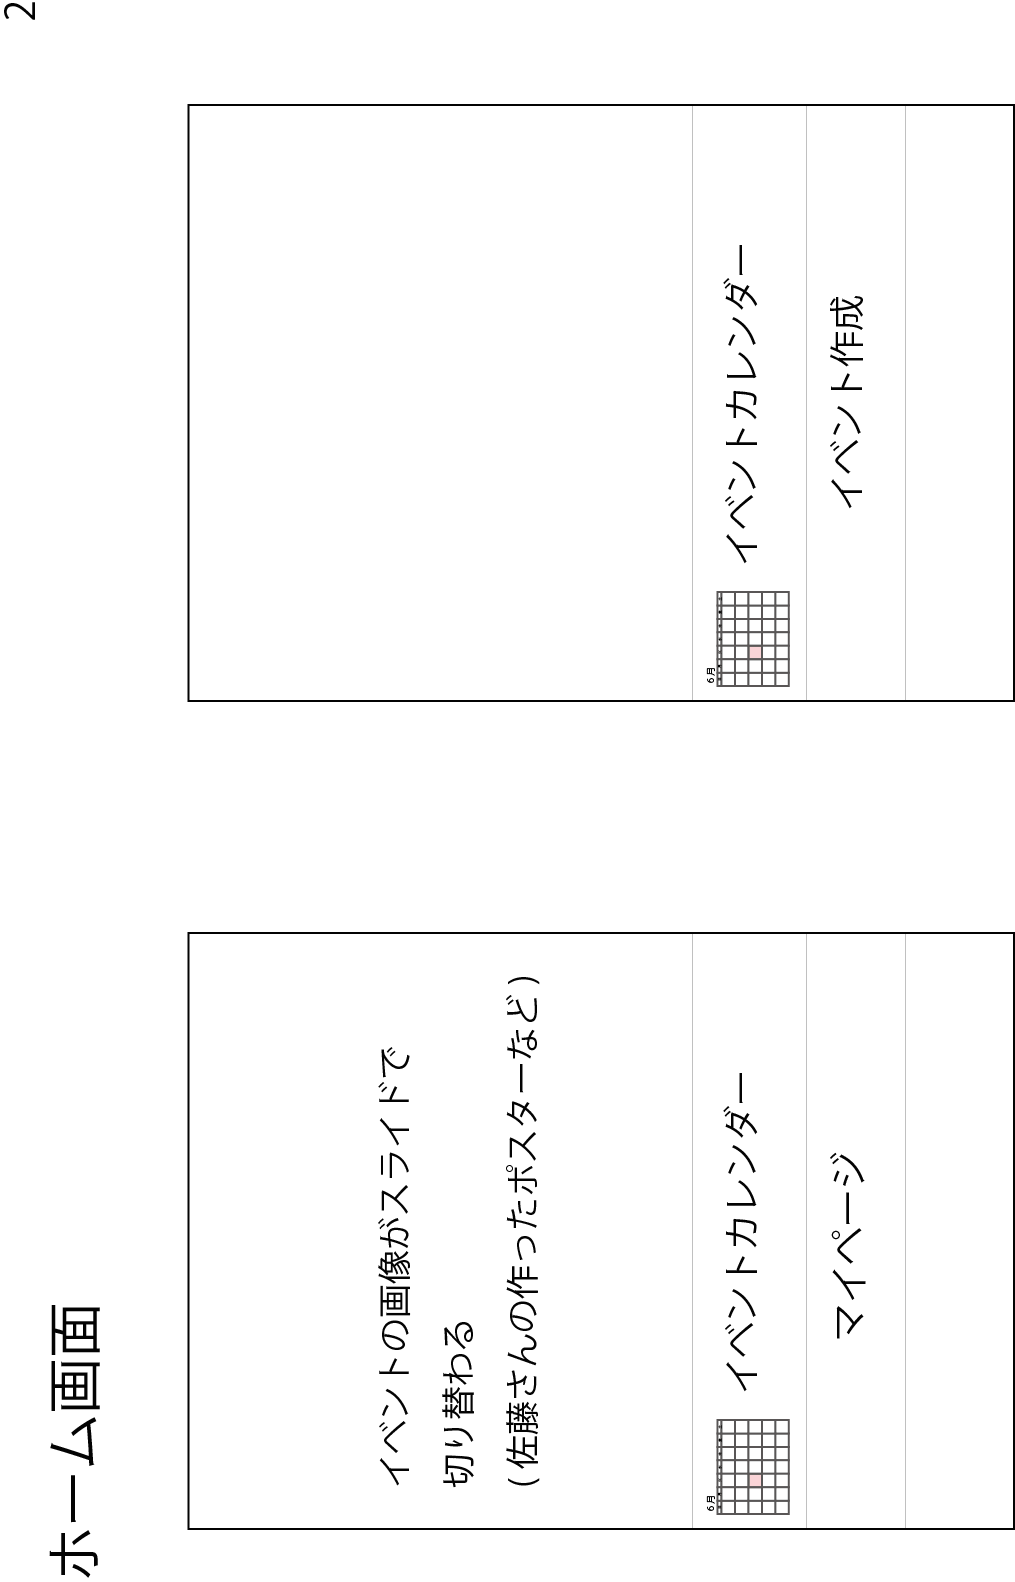
\includegraphics[keepaspectratio, scale=0.8]{appendixs/appendixA_figres/fig2.png}
    \end{center}
\end{figure}

\begin{figure}[ht]
    \begin{center}
      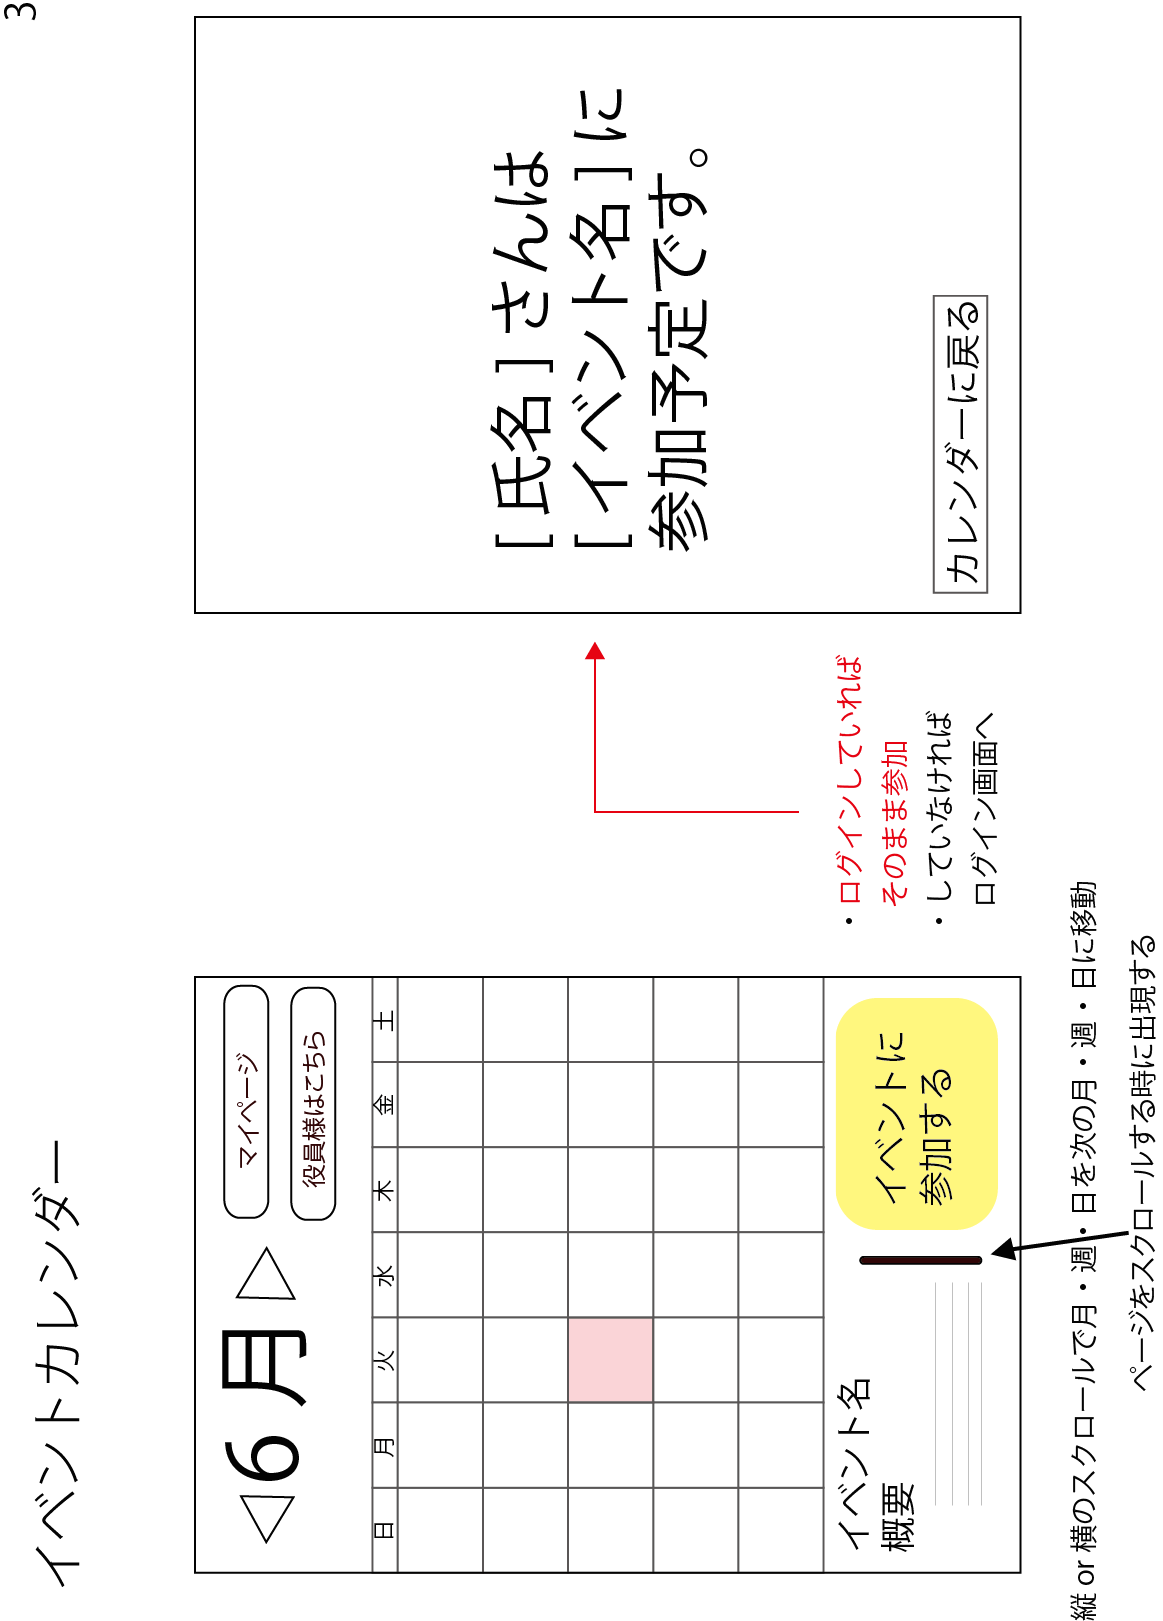
\includegraphics[keepaspectratio, scale=0.8]{appendixs/appendixA_figres/fig3.png}
    \end{center}
\end{figure}

\begin{figure}[ht]
    \begin{center}
    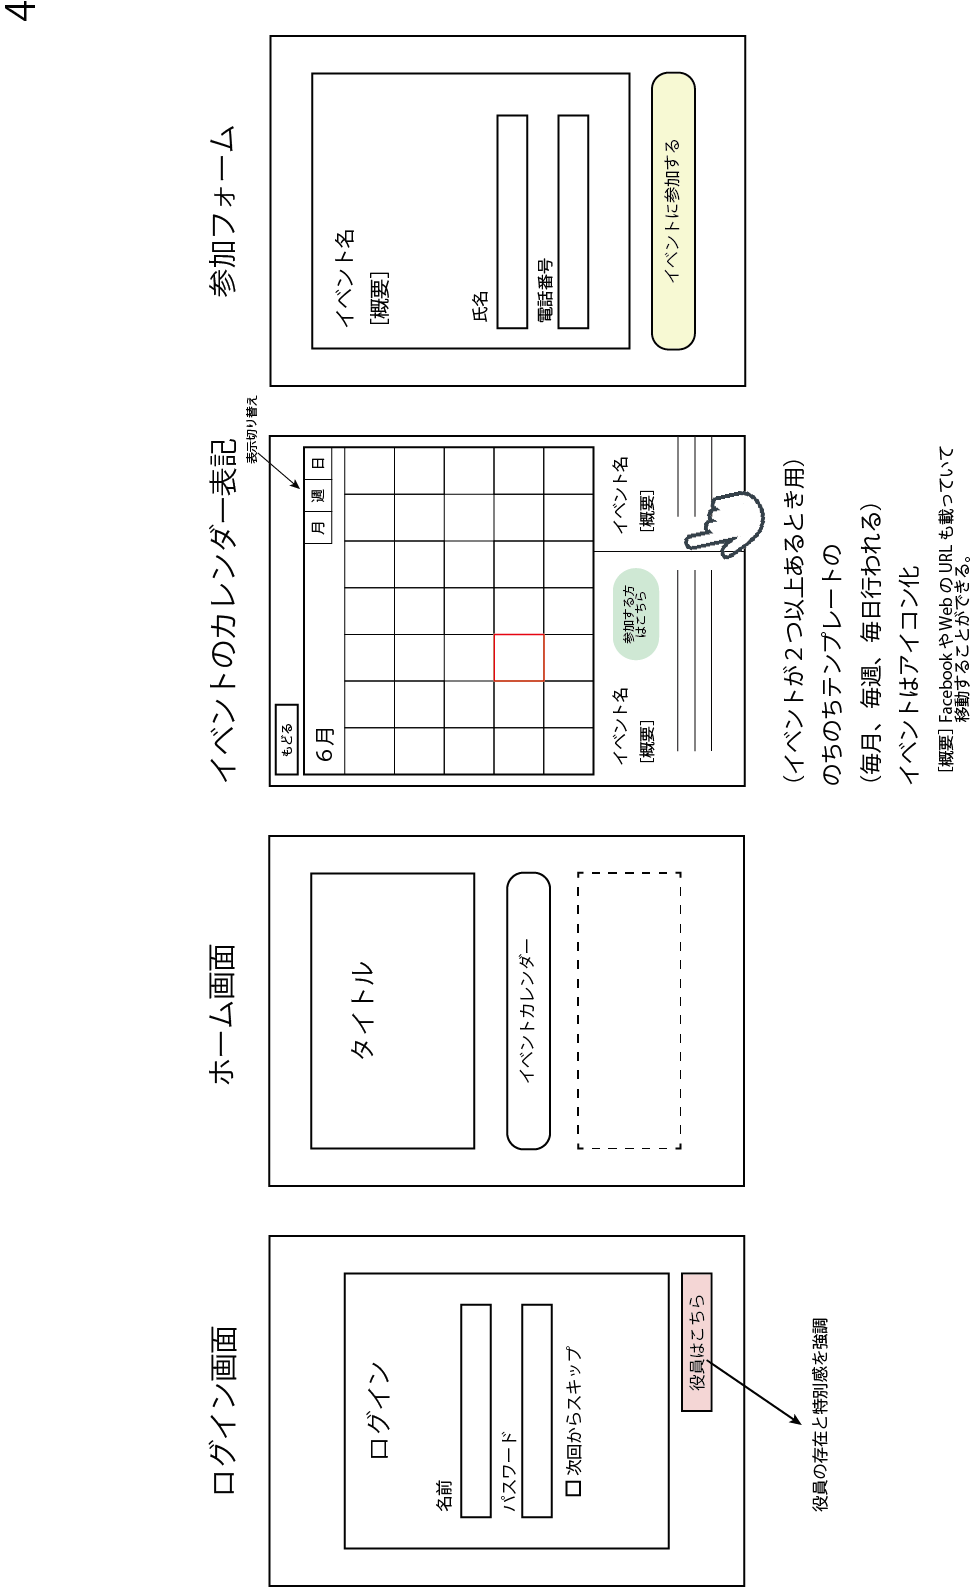
\includegraphics[keepaspectratio, scale=0.8]{appendixs/appendixA_figres/fig4.png}
    \end{center}
\end{figure}

\begin{figure}[ht]
    \begin{center}
      
\includegraphics[keepaspectratio, scale=0.8]{appendixs/appendixA_figres/fig5.png}
    \end{center}
\end{figure}


\chapter{6月23日提案資料}
\begin{figure}[ht]
    \begin{center}
      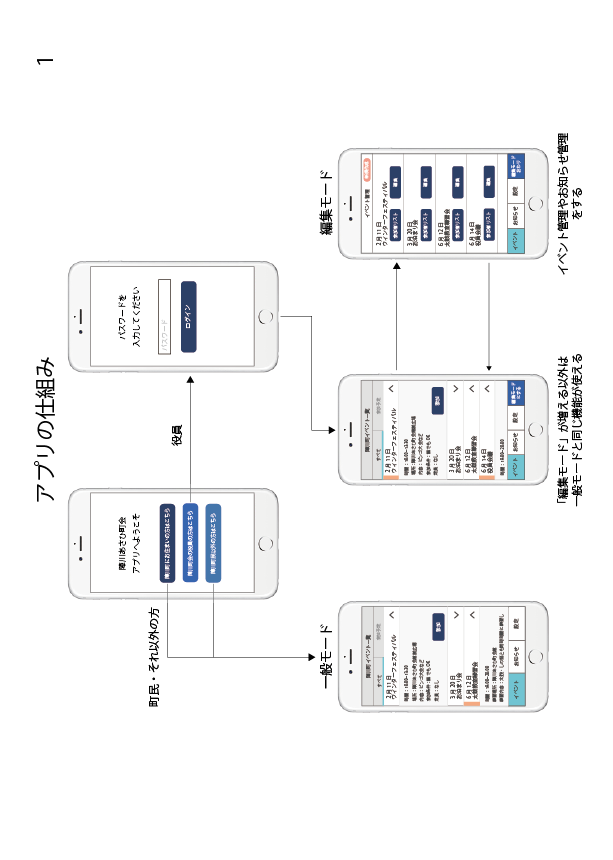
\includegraphics[keepaspectratio, scale=0.65]{appendixs/appendixB_figres/fig1.png}
    \end{center}
\end{figure}

\begin{figure}[ht]
    \begin{center}
    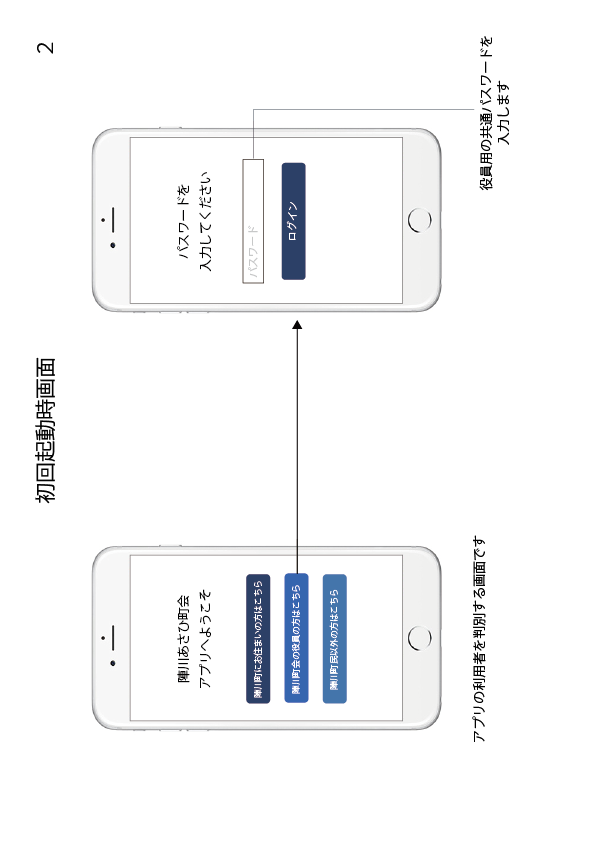
\includegraphics[keepaspectratio, scale=0.7]{appendixs/appendixB_figres/fig2.png}
    \end{center}
\end{figure}

\begin{figure}[ht]
    \begin{center}
      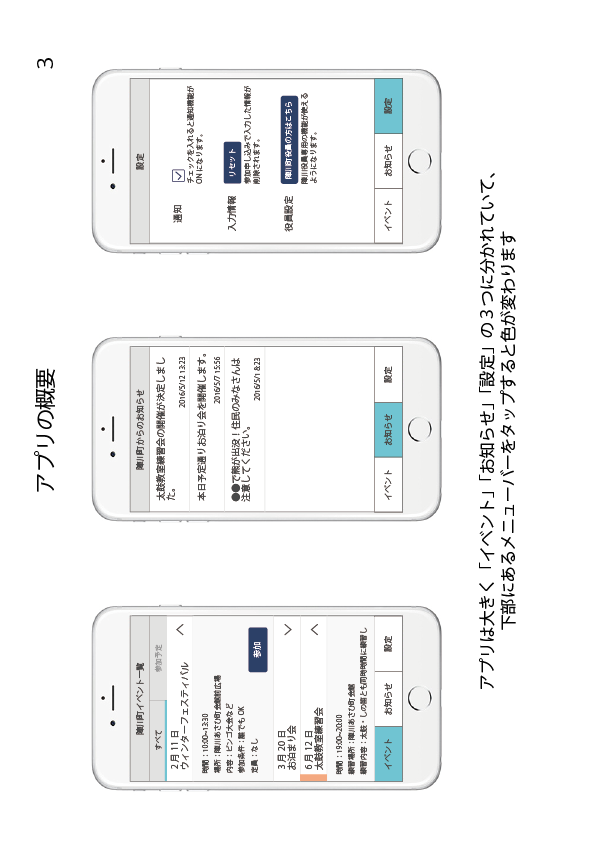
\includegraphics[keepaspectratio, scale=0.7]{appendixs/appendixB_figres/fig3.png}
    \end{center}
\end{figure}

\begin{figure}[ht]
    \begin{center}
    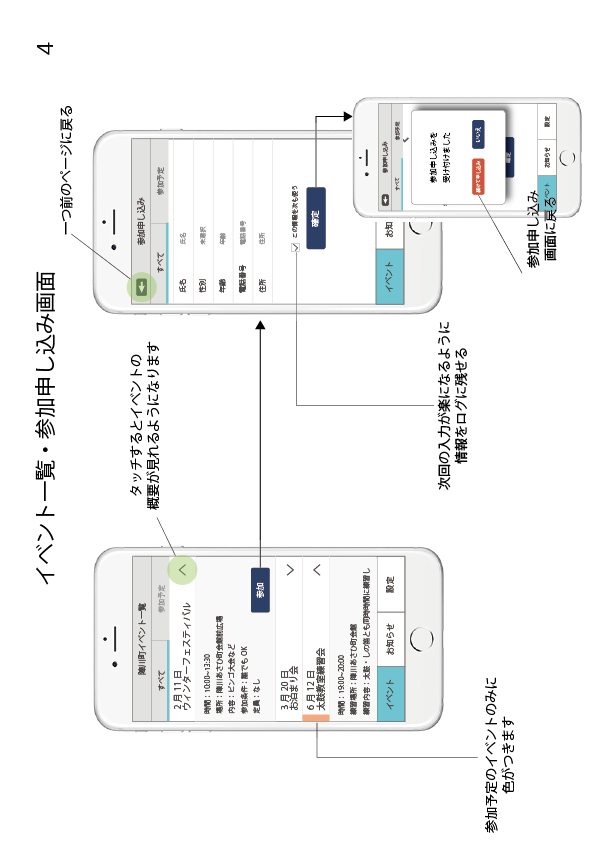
\includegraphics[keepaspectratio, scale=0.7]{appendixs/appendixB_figres/fig4.png}
    \end{center}
\end{figure}

\begin{figure}[ht]
    \begin{center}
      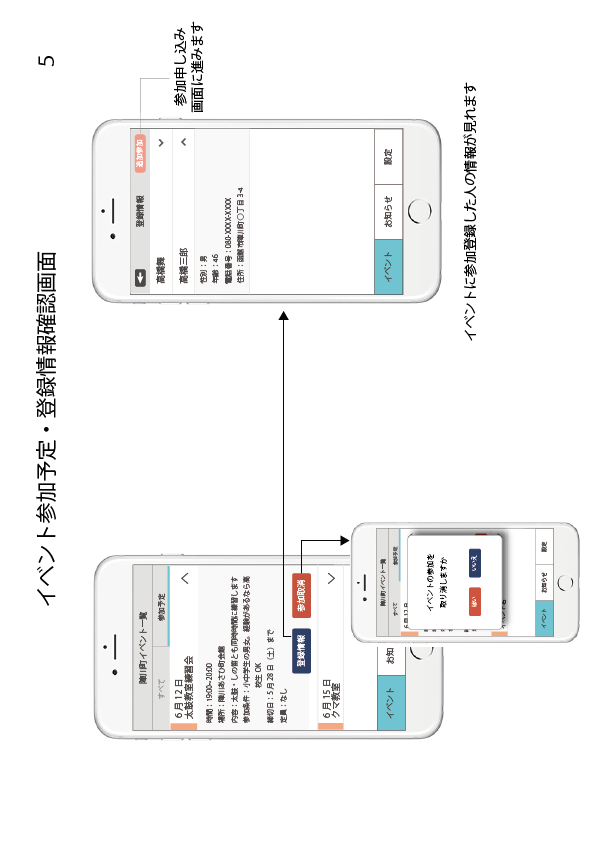
\includegraphics[keepaspectratio, scale=0.7]{appendixs/appendixB_figres/fig5.png}
    \end{center}
\end{figure}

\begin{figure}[ht]
    \begin{center}
    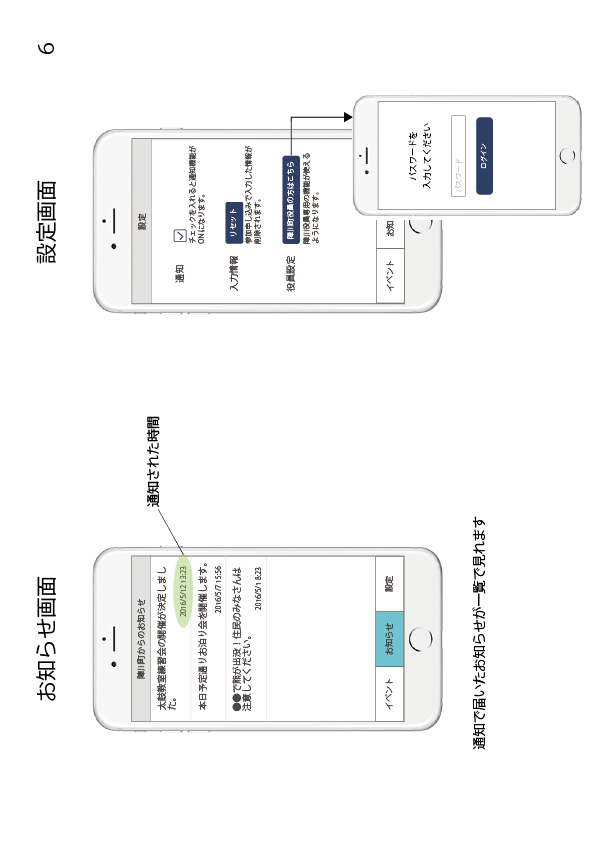
\includegraphics[keepaspectratio, scale=0.7]{appendixs/appendixB_figres/fig6.png}
    \end{center}
\end{figure}

\begin{figure}[ht]
    \begin{center}
      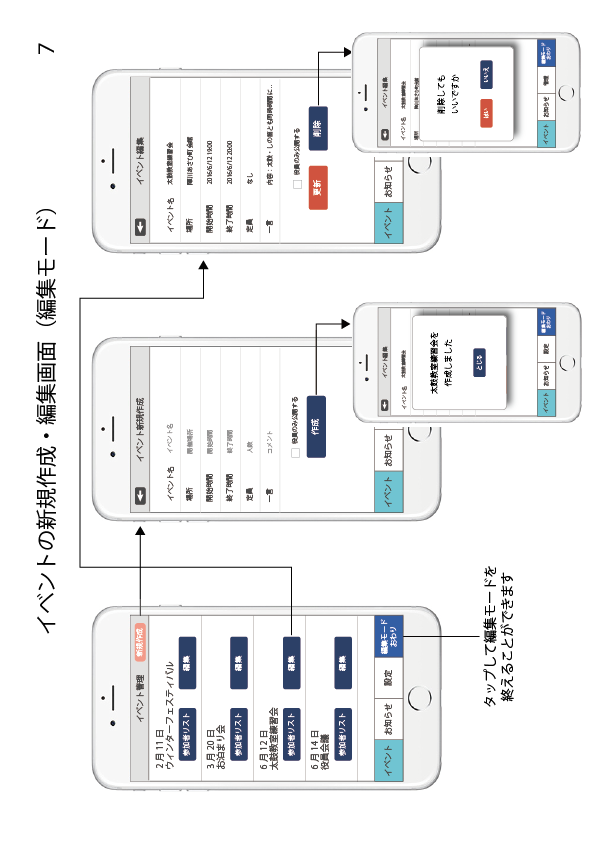
\includegraphics[keepaspectratio, scale=0.7]{appendixs/appendixB_figres/fig7.png}
    \end{center}
\end{figure}

\begin{figure}[ht]
    \begin{center}
    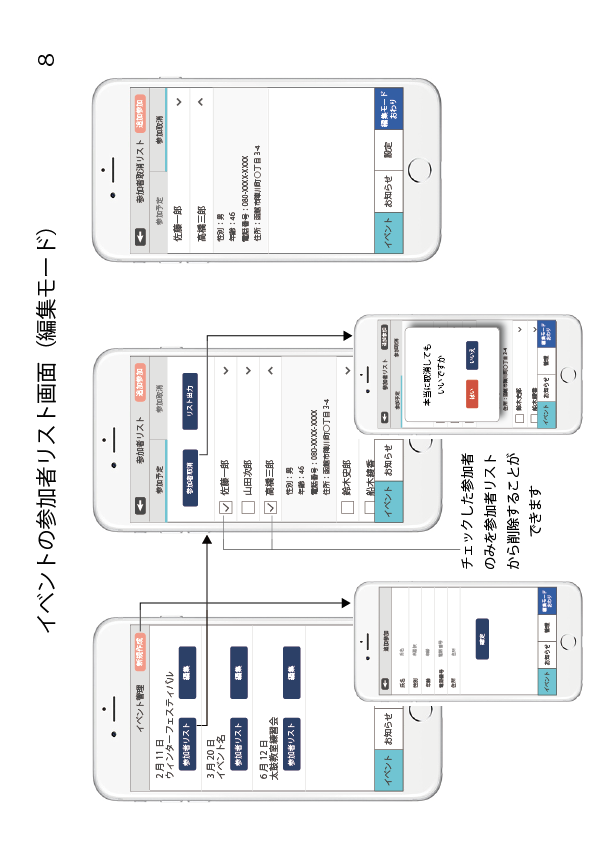
\includegraphics[keepaspectratio, scale=0.7]{appendixs/appendixB_figres/fig8.png}
    \end{center}
\end{figure}

\begin{figure}[ht]
    \begin{center}
      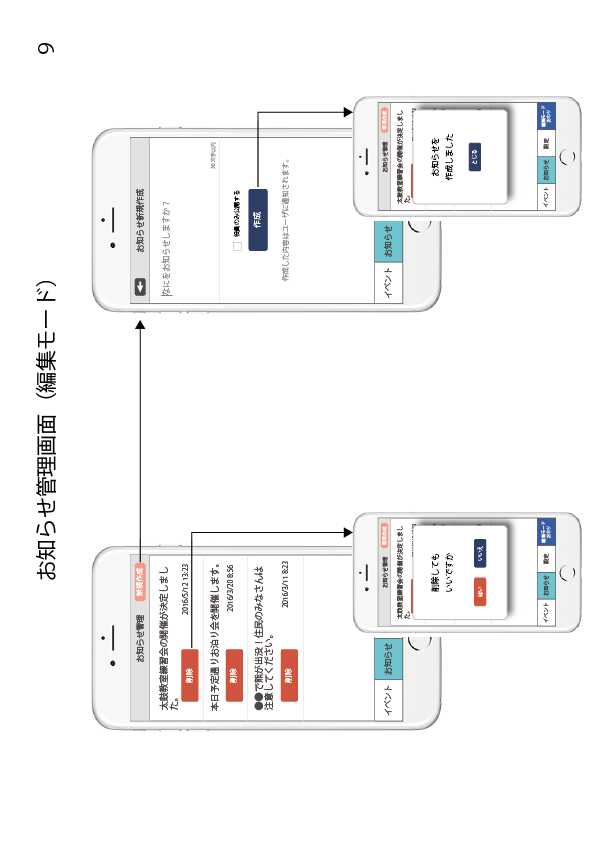
\includegraphics[keepaspectratio, scale=0.7]{appendixs/appendixB_figres/fig9.png}
    \end{center}
\end{figure}


\chapter{11月18日提案資料}
\begin{figure}[ht]
    \begin{center}
      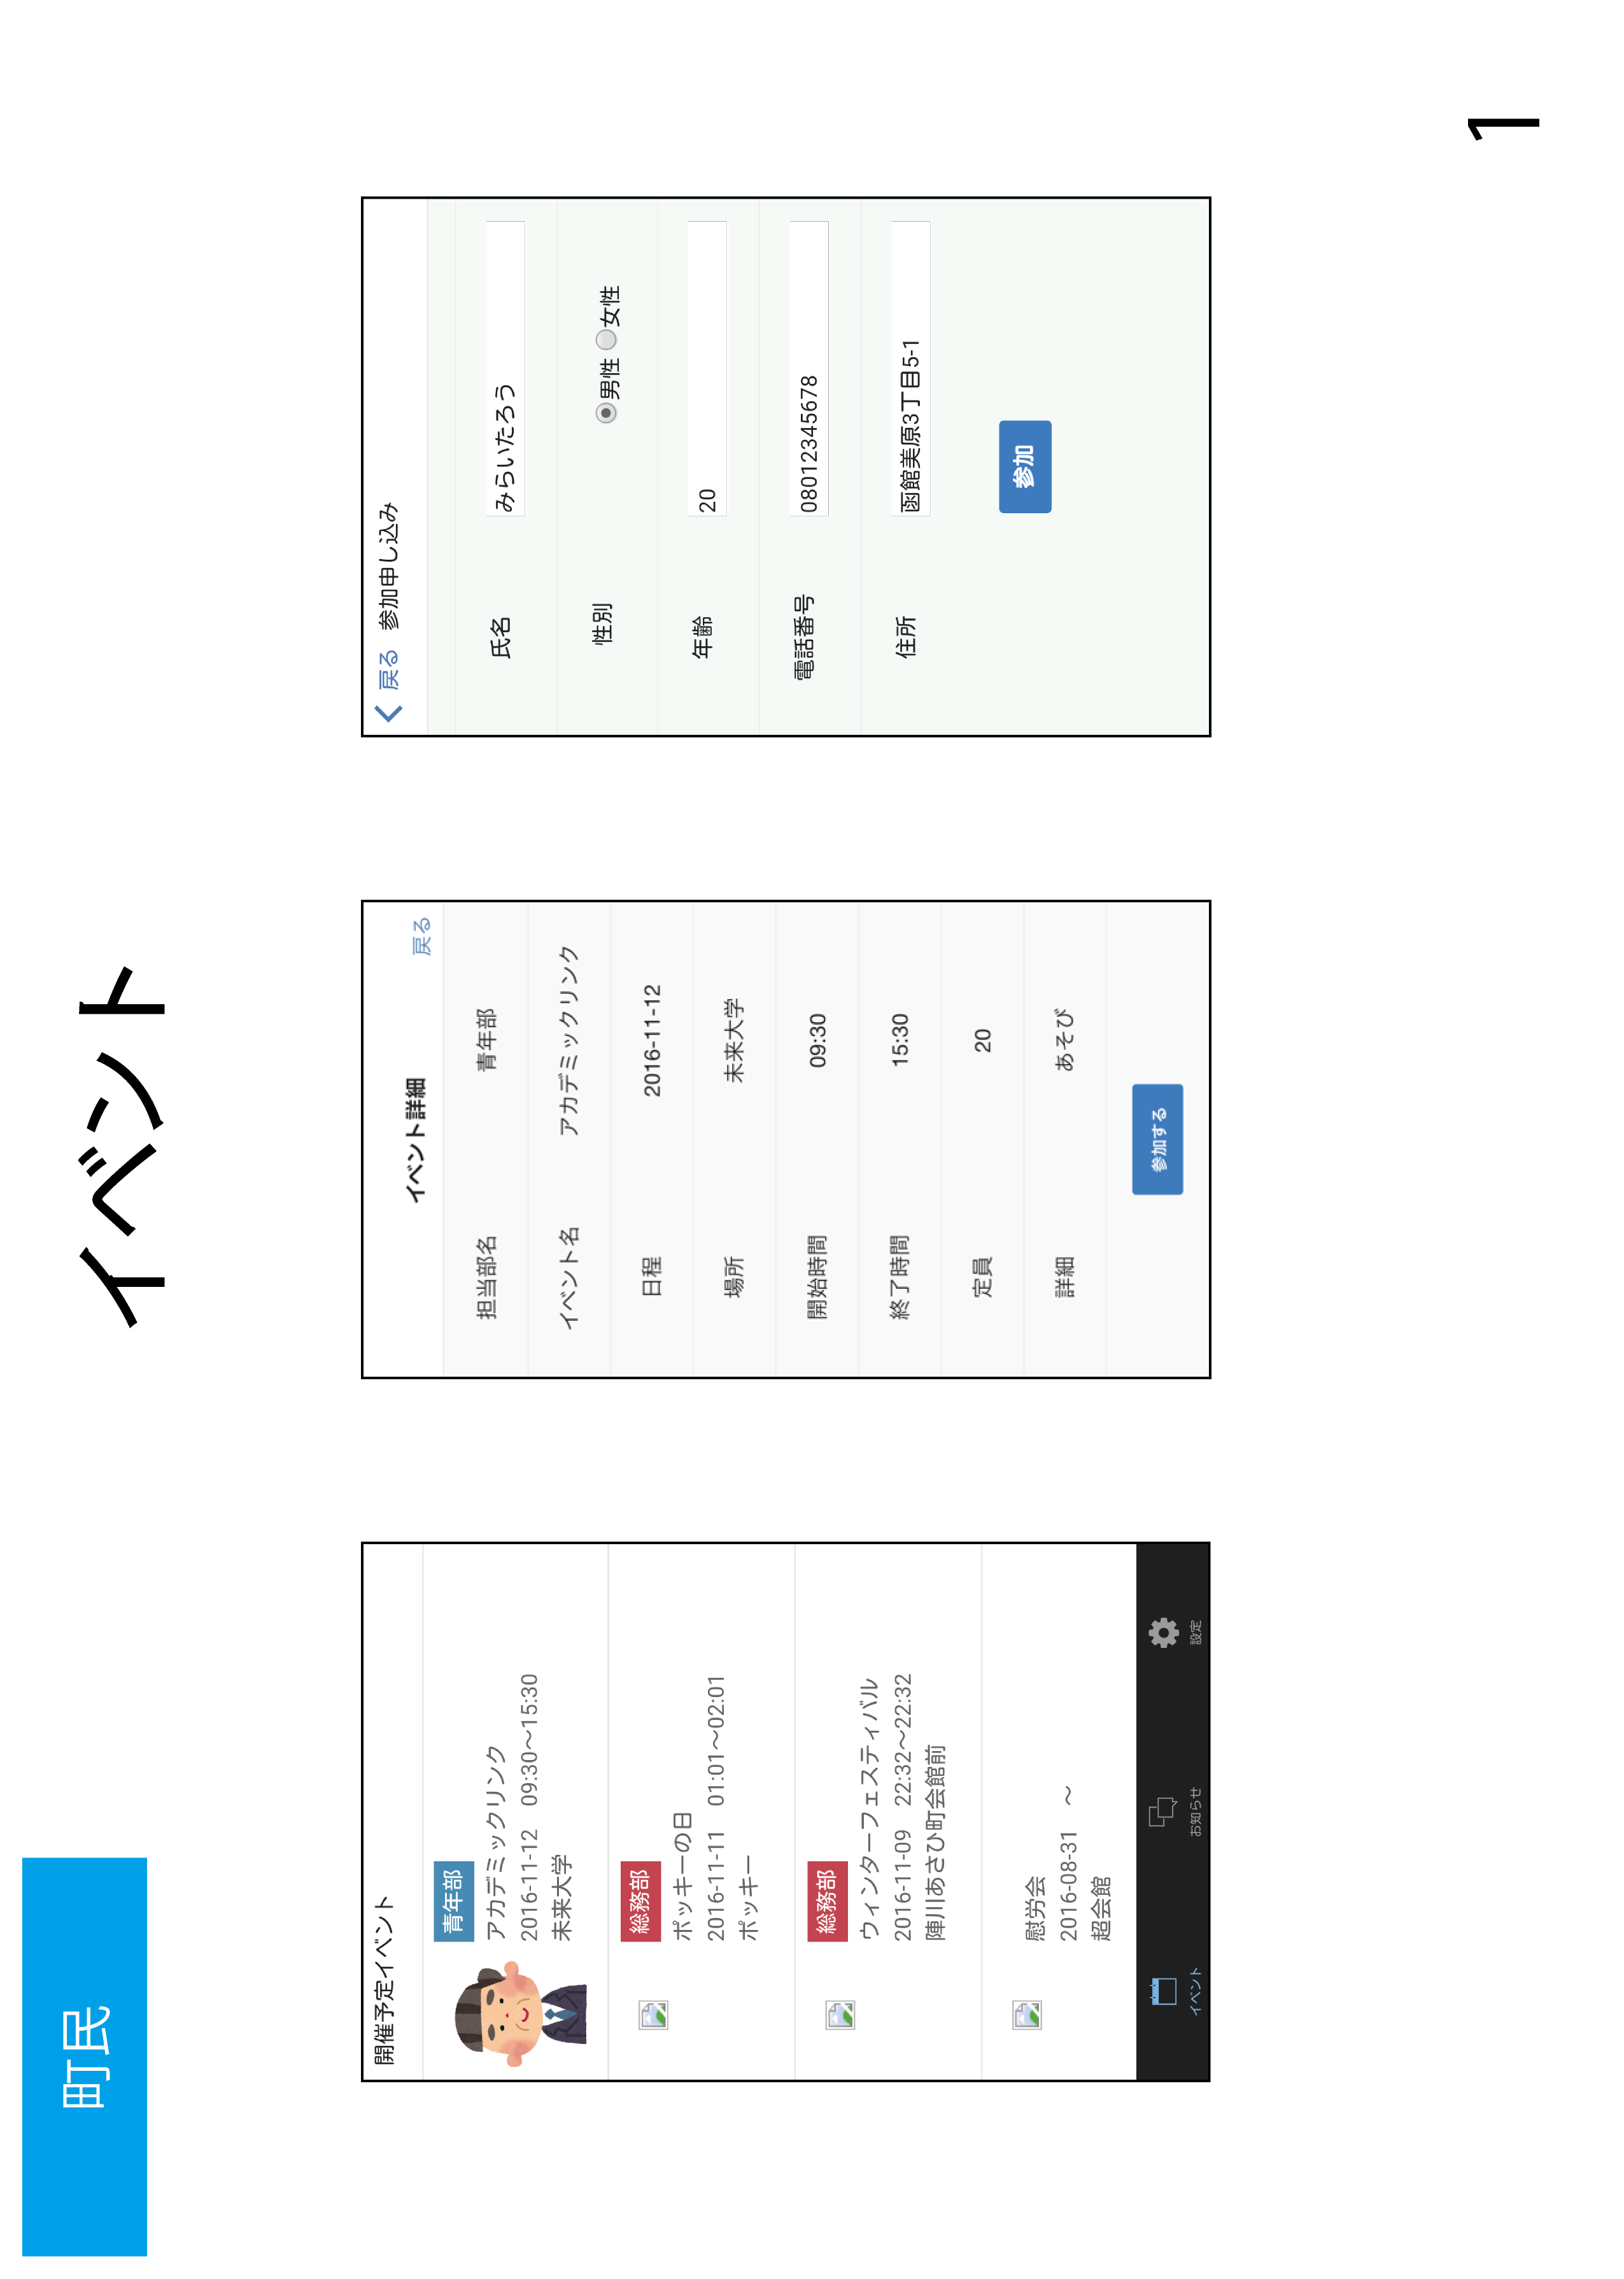
\includegraphics[keepaspectratio, scale=0.65]{appendix11_18-01.png}
    \end{center}
\end{figure}

\begin{figure}[ht]
    \begin{center}
    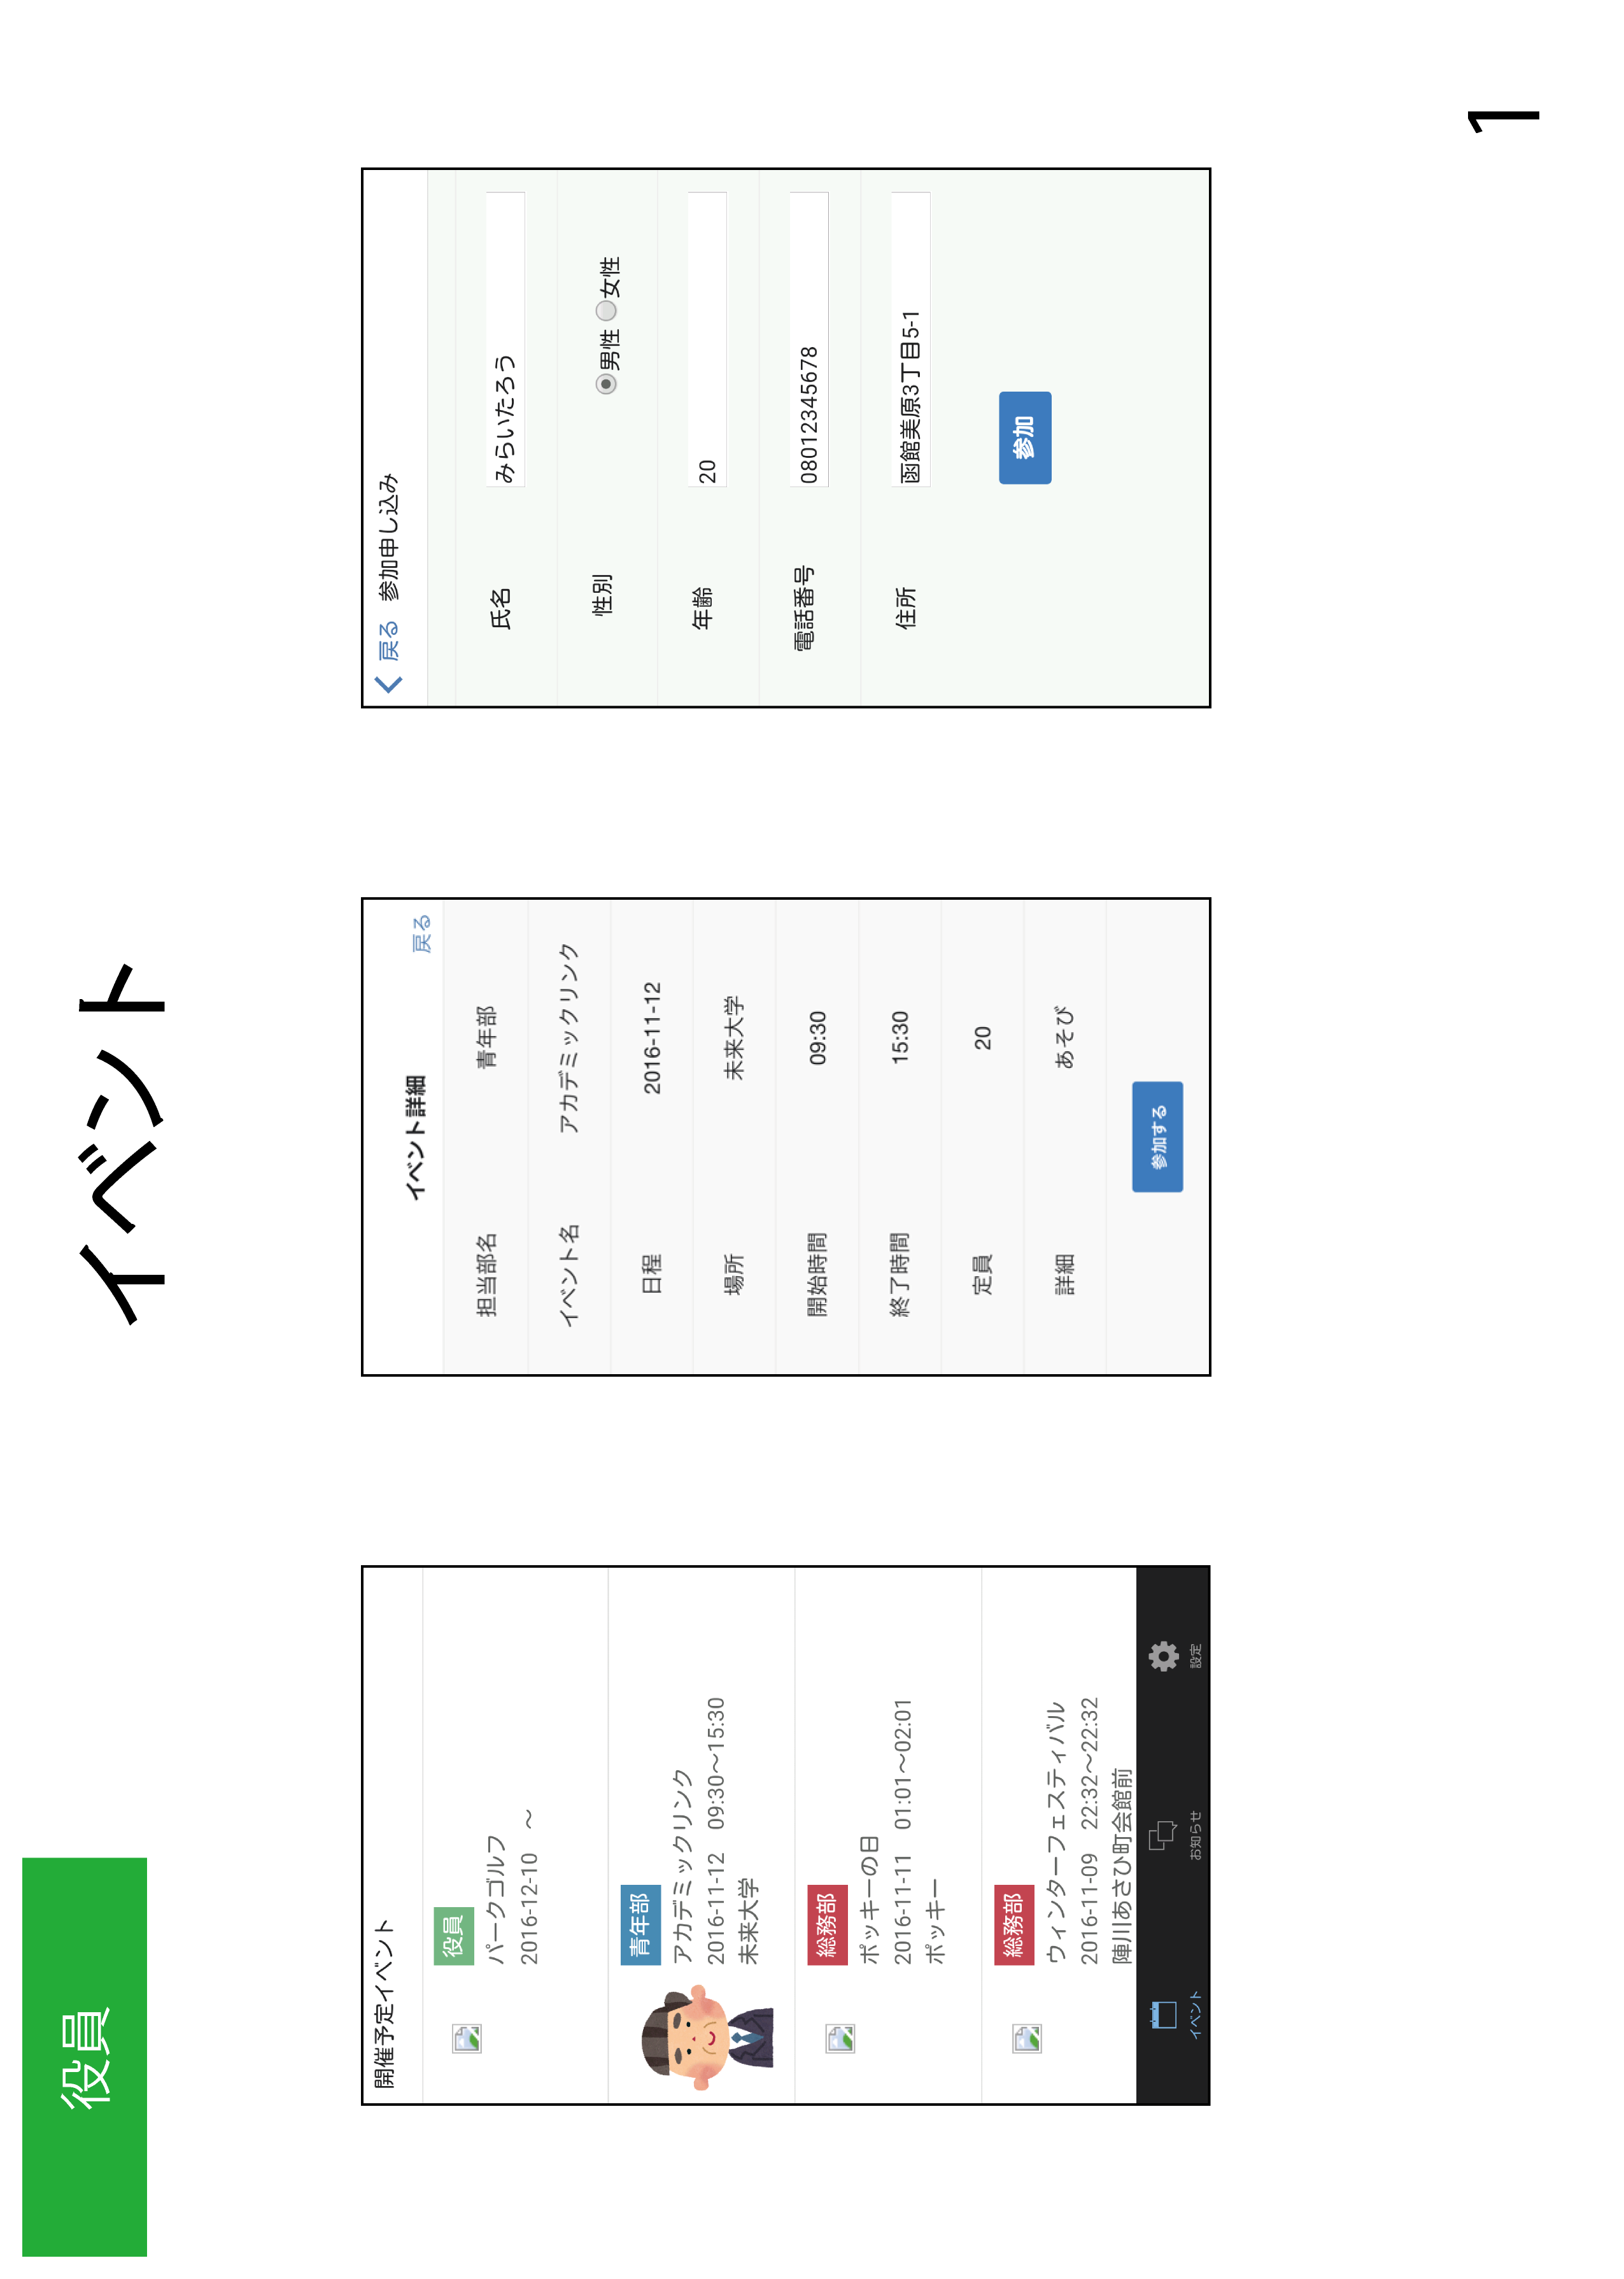
\includegraphics[keepaspectratio, scale=0.7]{appendix11_18-02.png}
    \end{center}
\end{figure}

\begin{figure}[ht]
    \begin{center}
      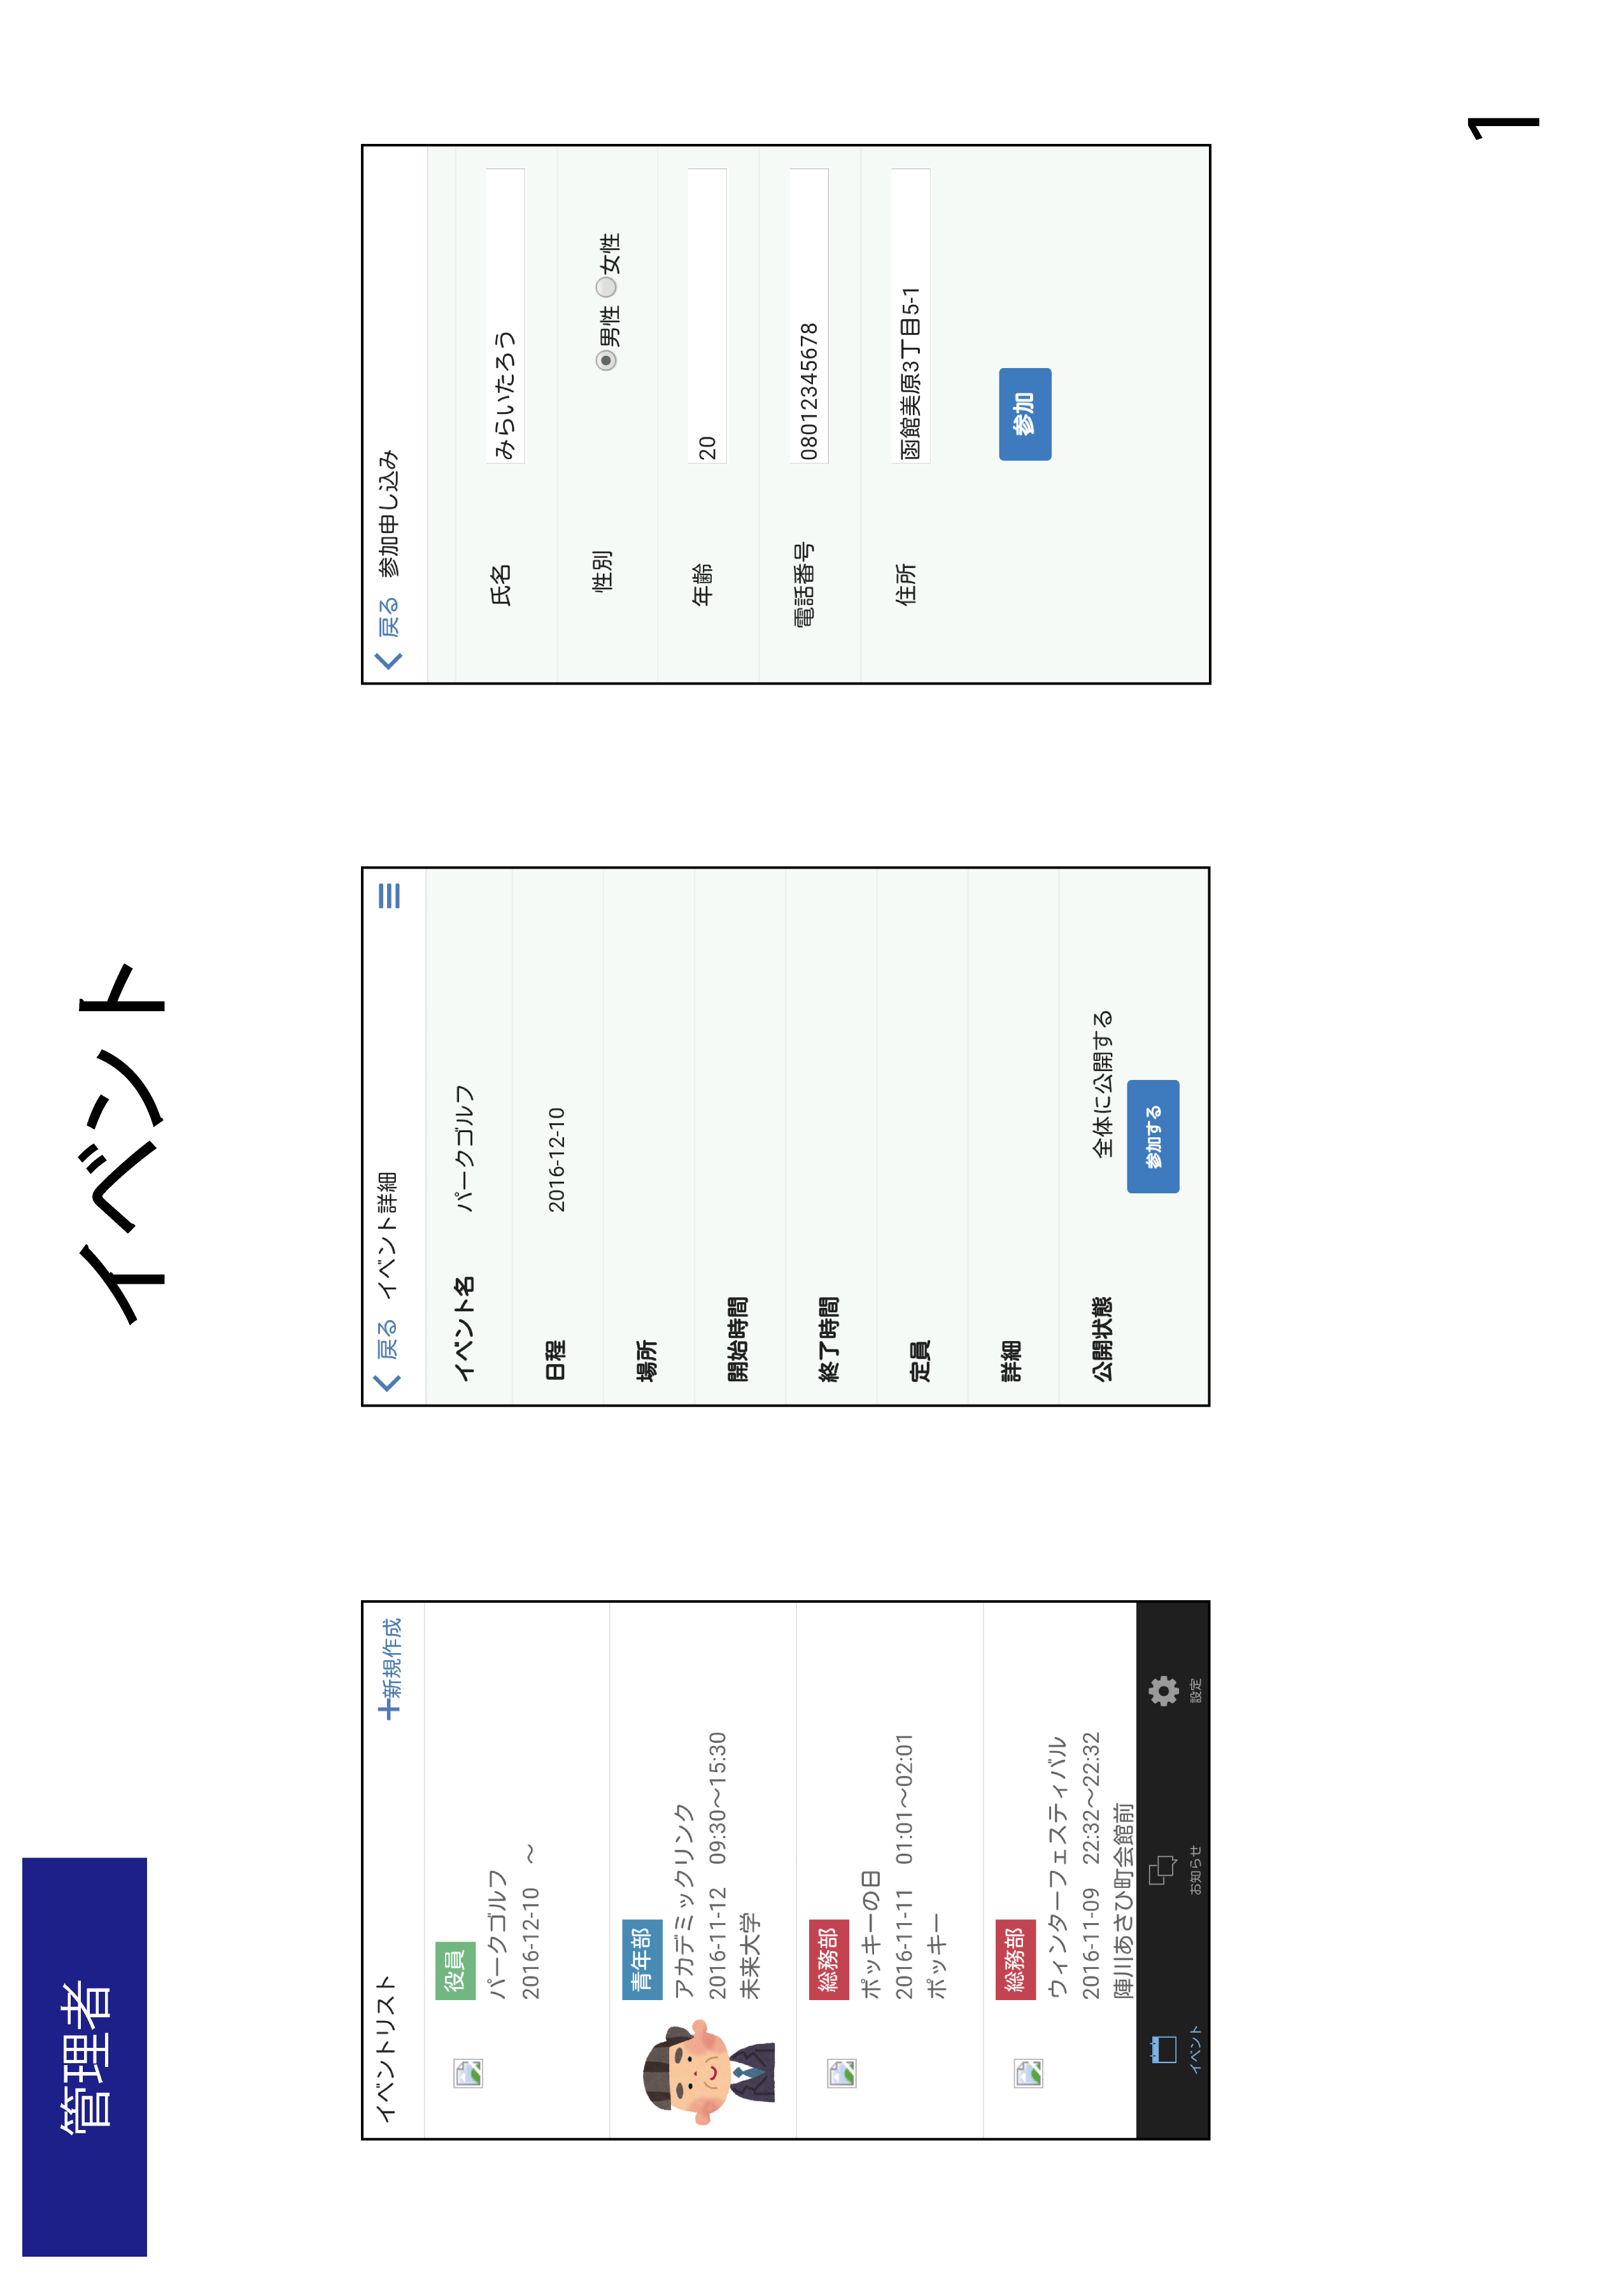
\includegraphics[keepaspectratio, scale=0.7]{appendix11_18-03.png}
    \end{center}
\end{figure}

\begin{figure}[ht]
    \begin{center}
    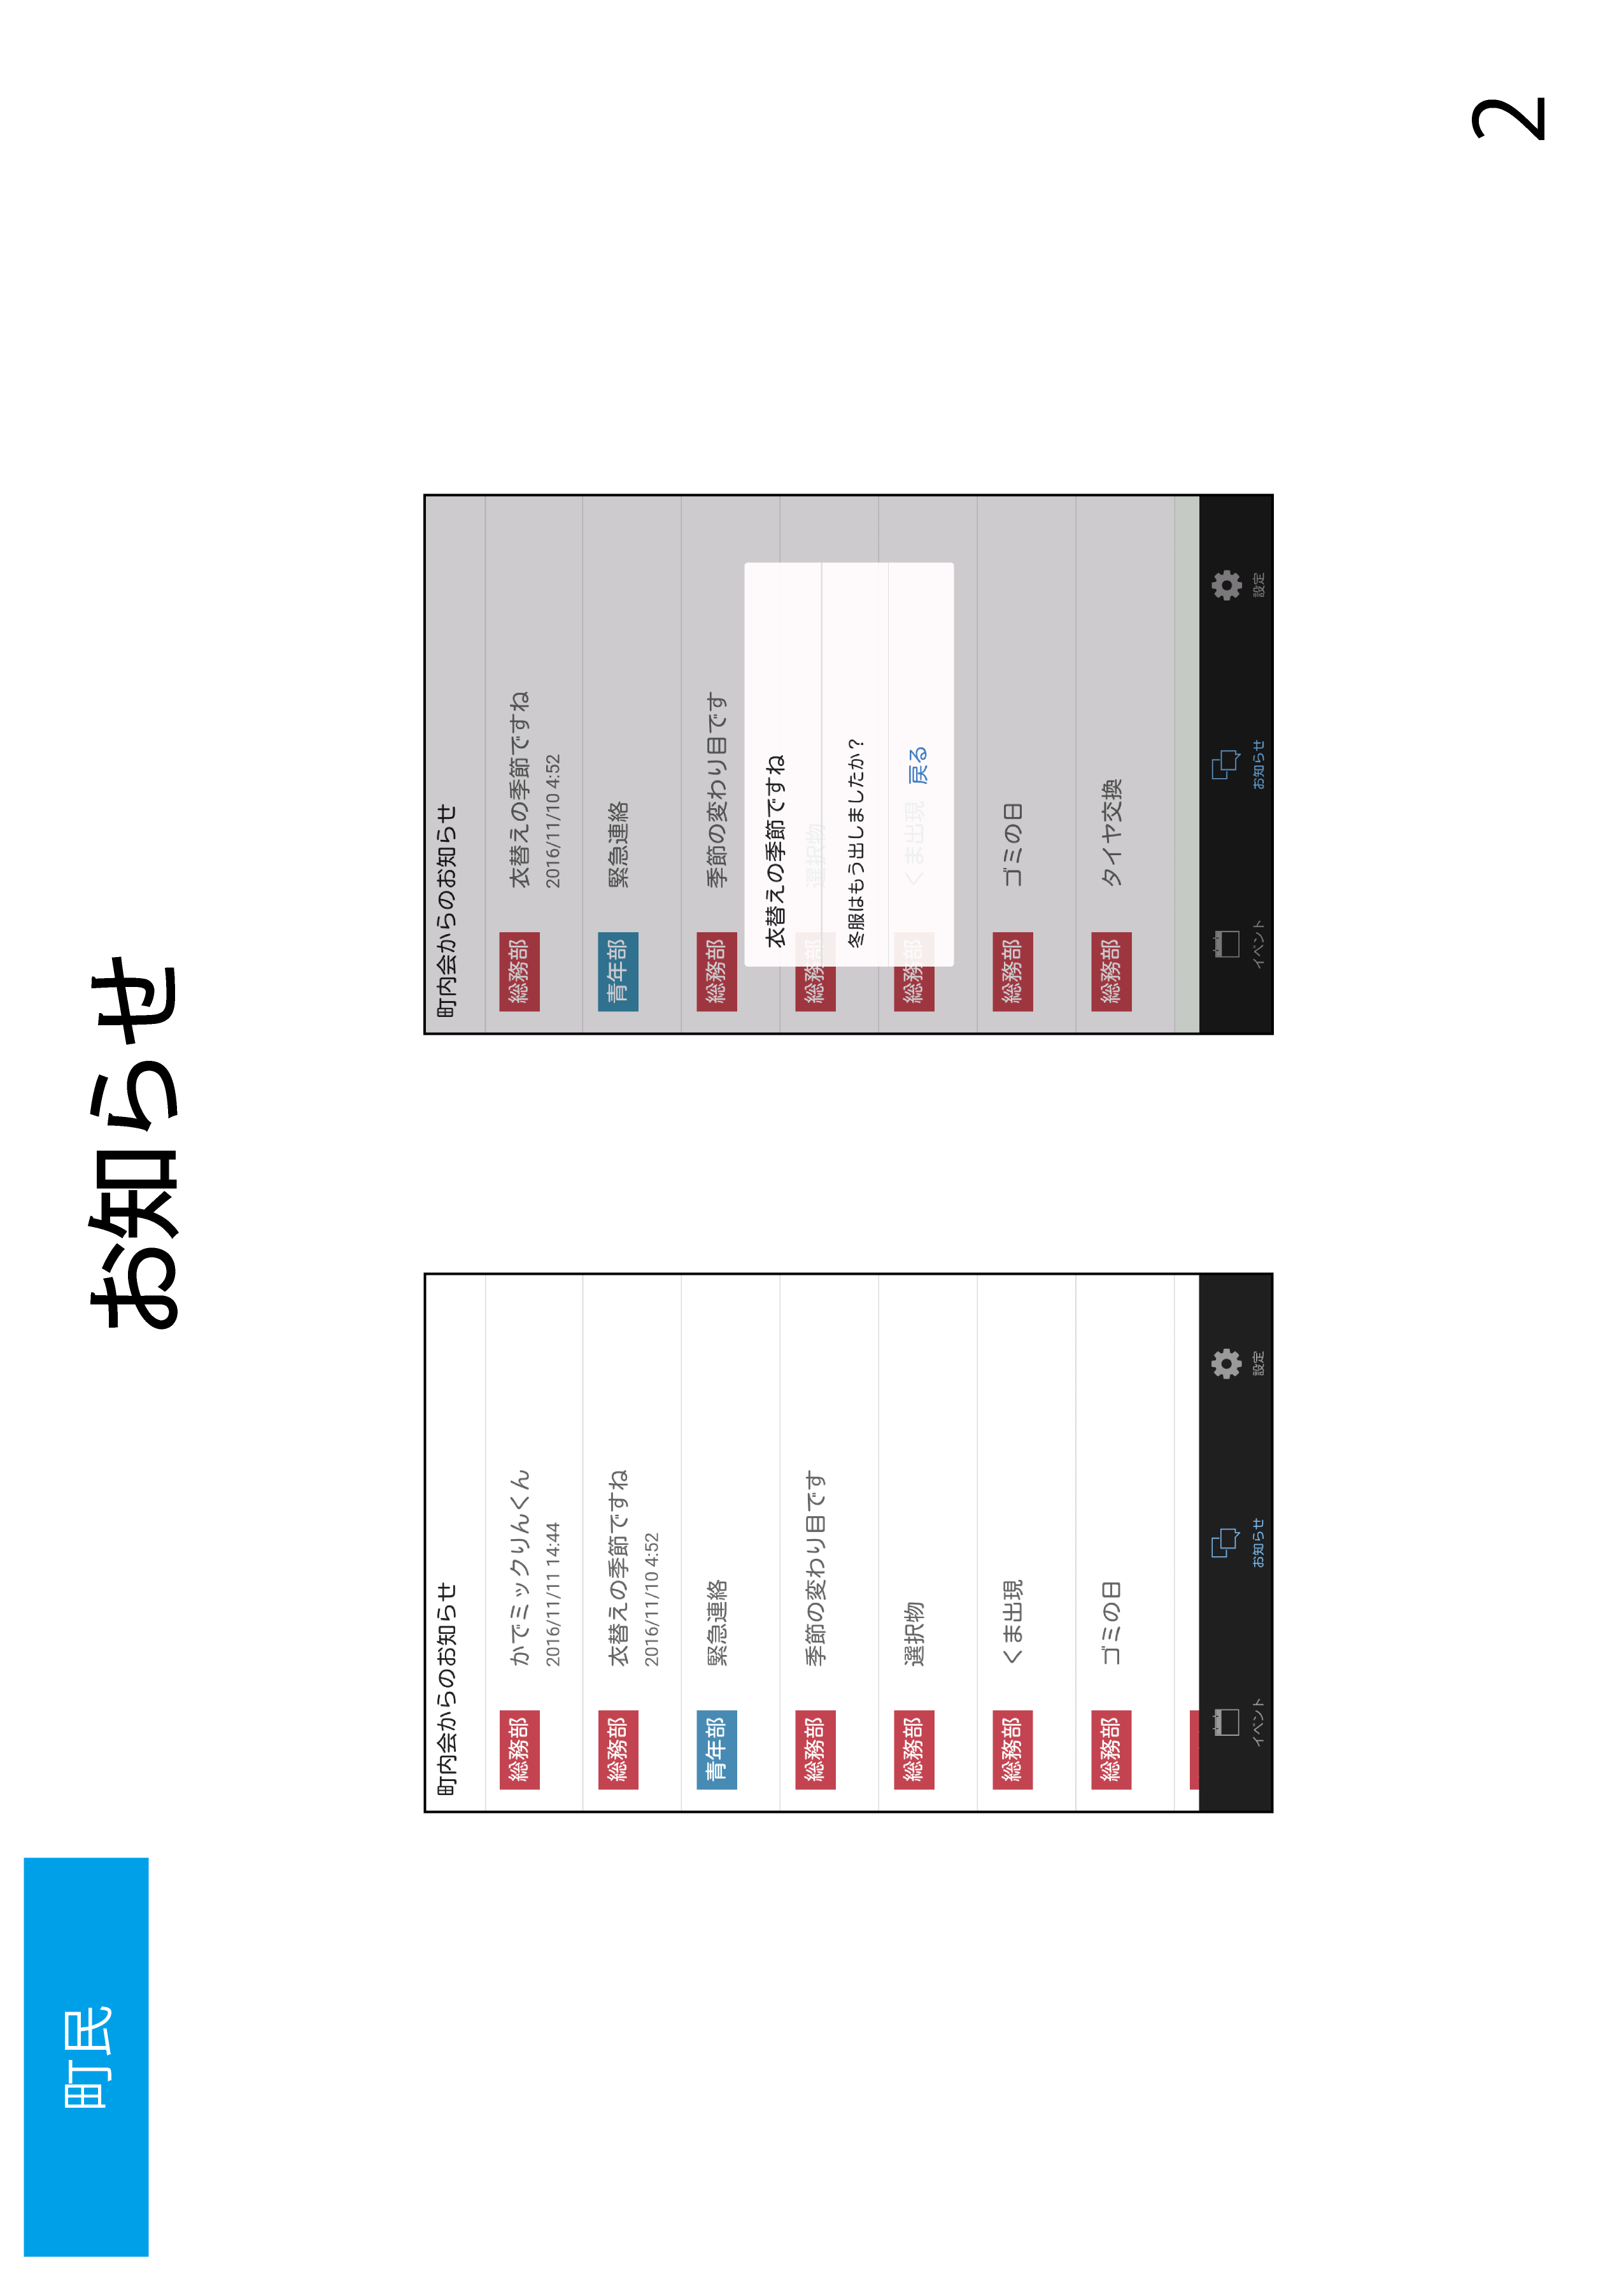
\includegraphics[keepaspectratio, scale=0.7]{appendix11_18-04.png}
    \end{center}
\end{figure}

\begin{figure}[ht]
    \begin{center}
      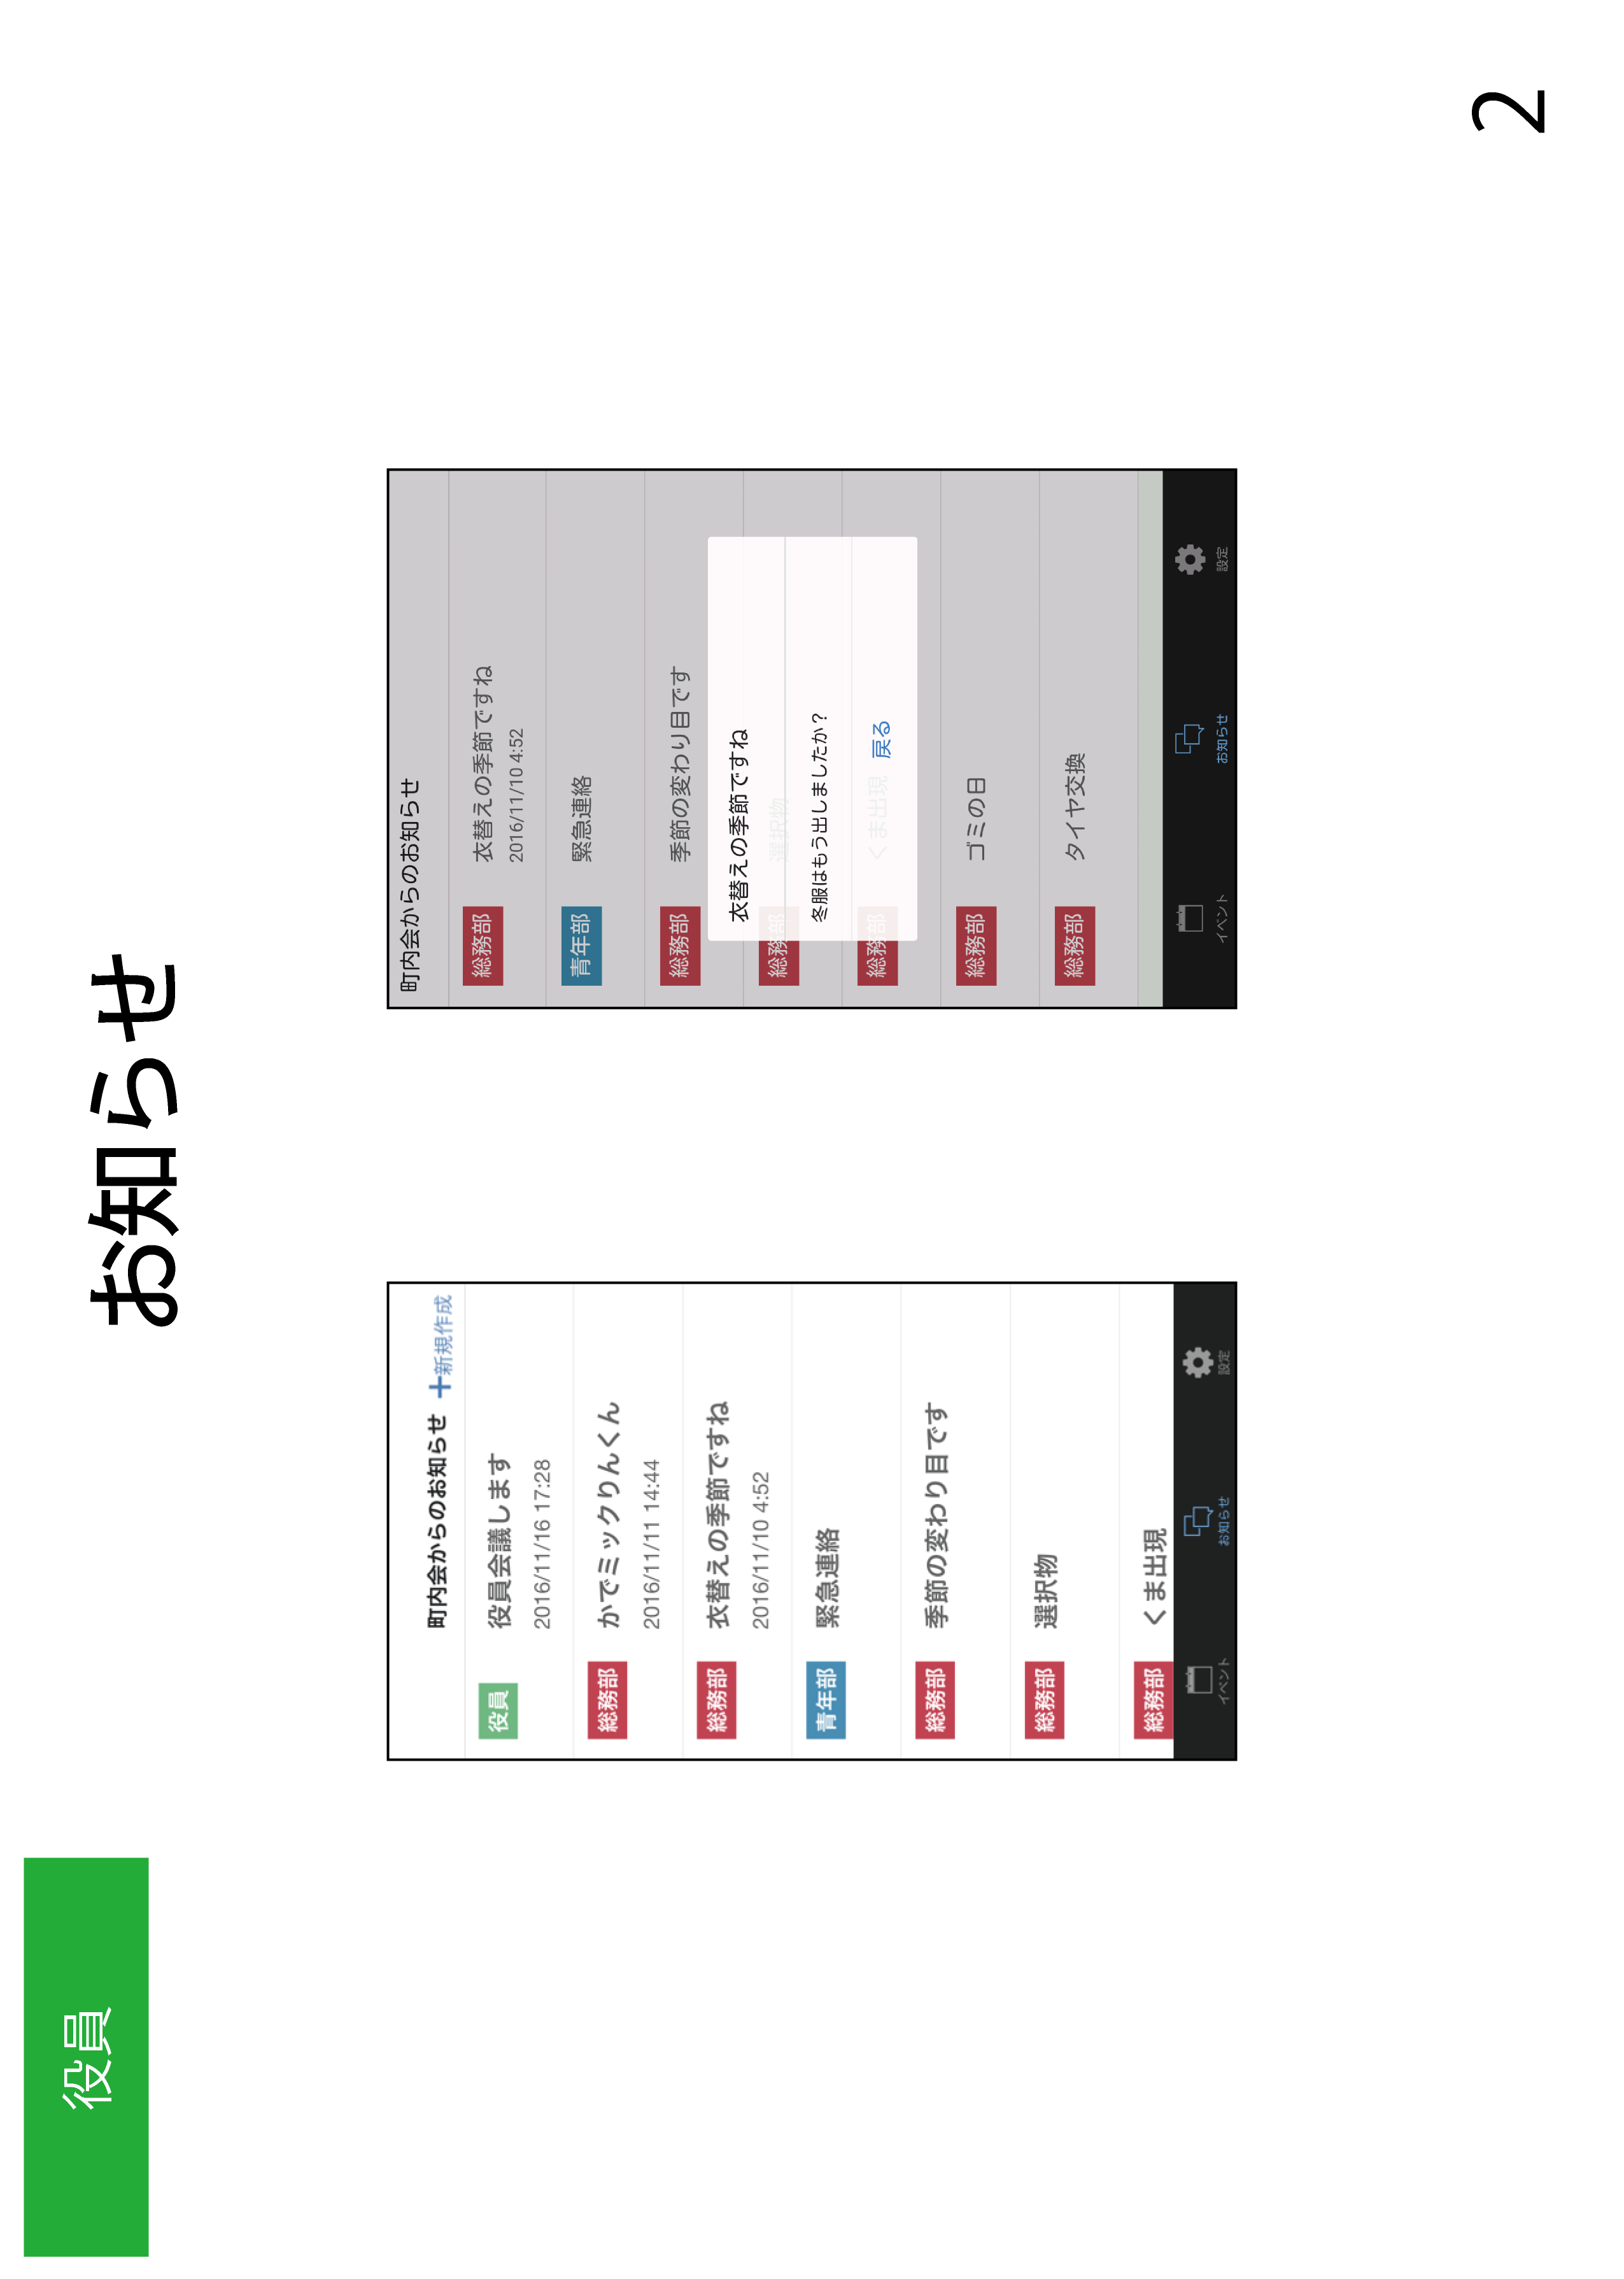
\includegraphics[keepaspectratio, scale=0.7]{appendix11_18-05.png}
    \end{center}
\end{figure}

\begin{figure}[ht]
    \begin{center}
    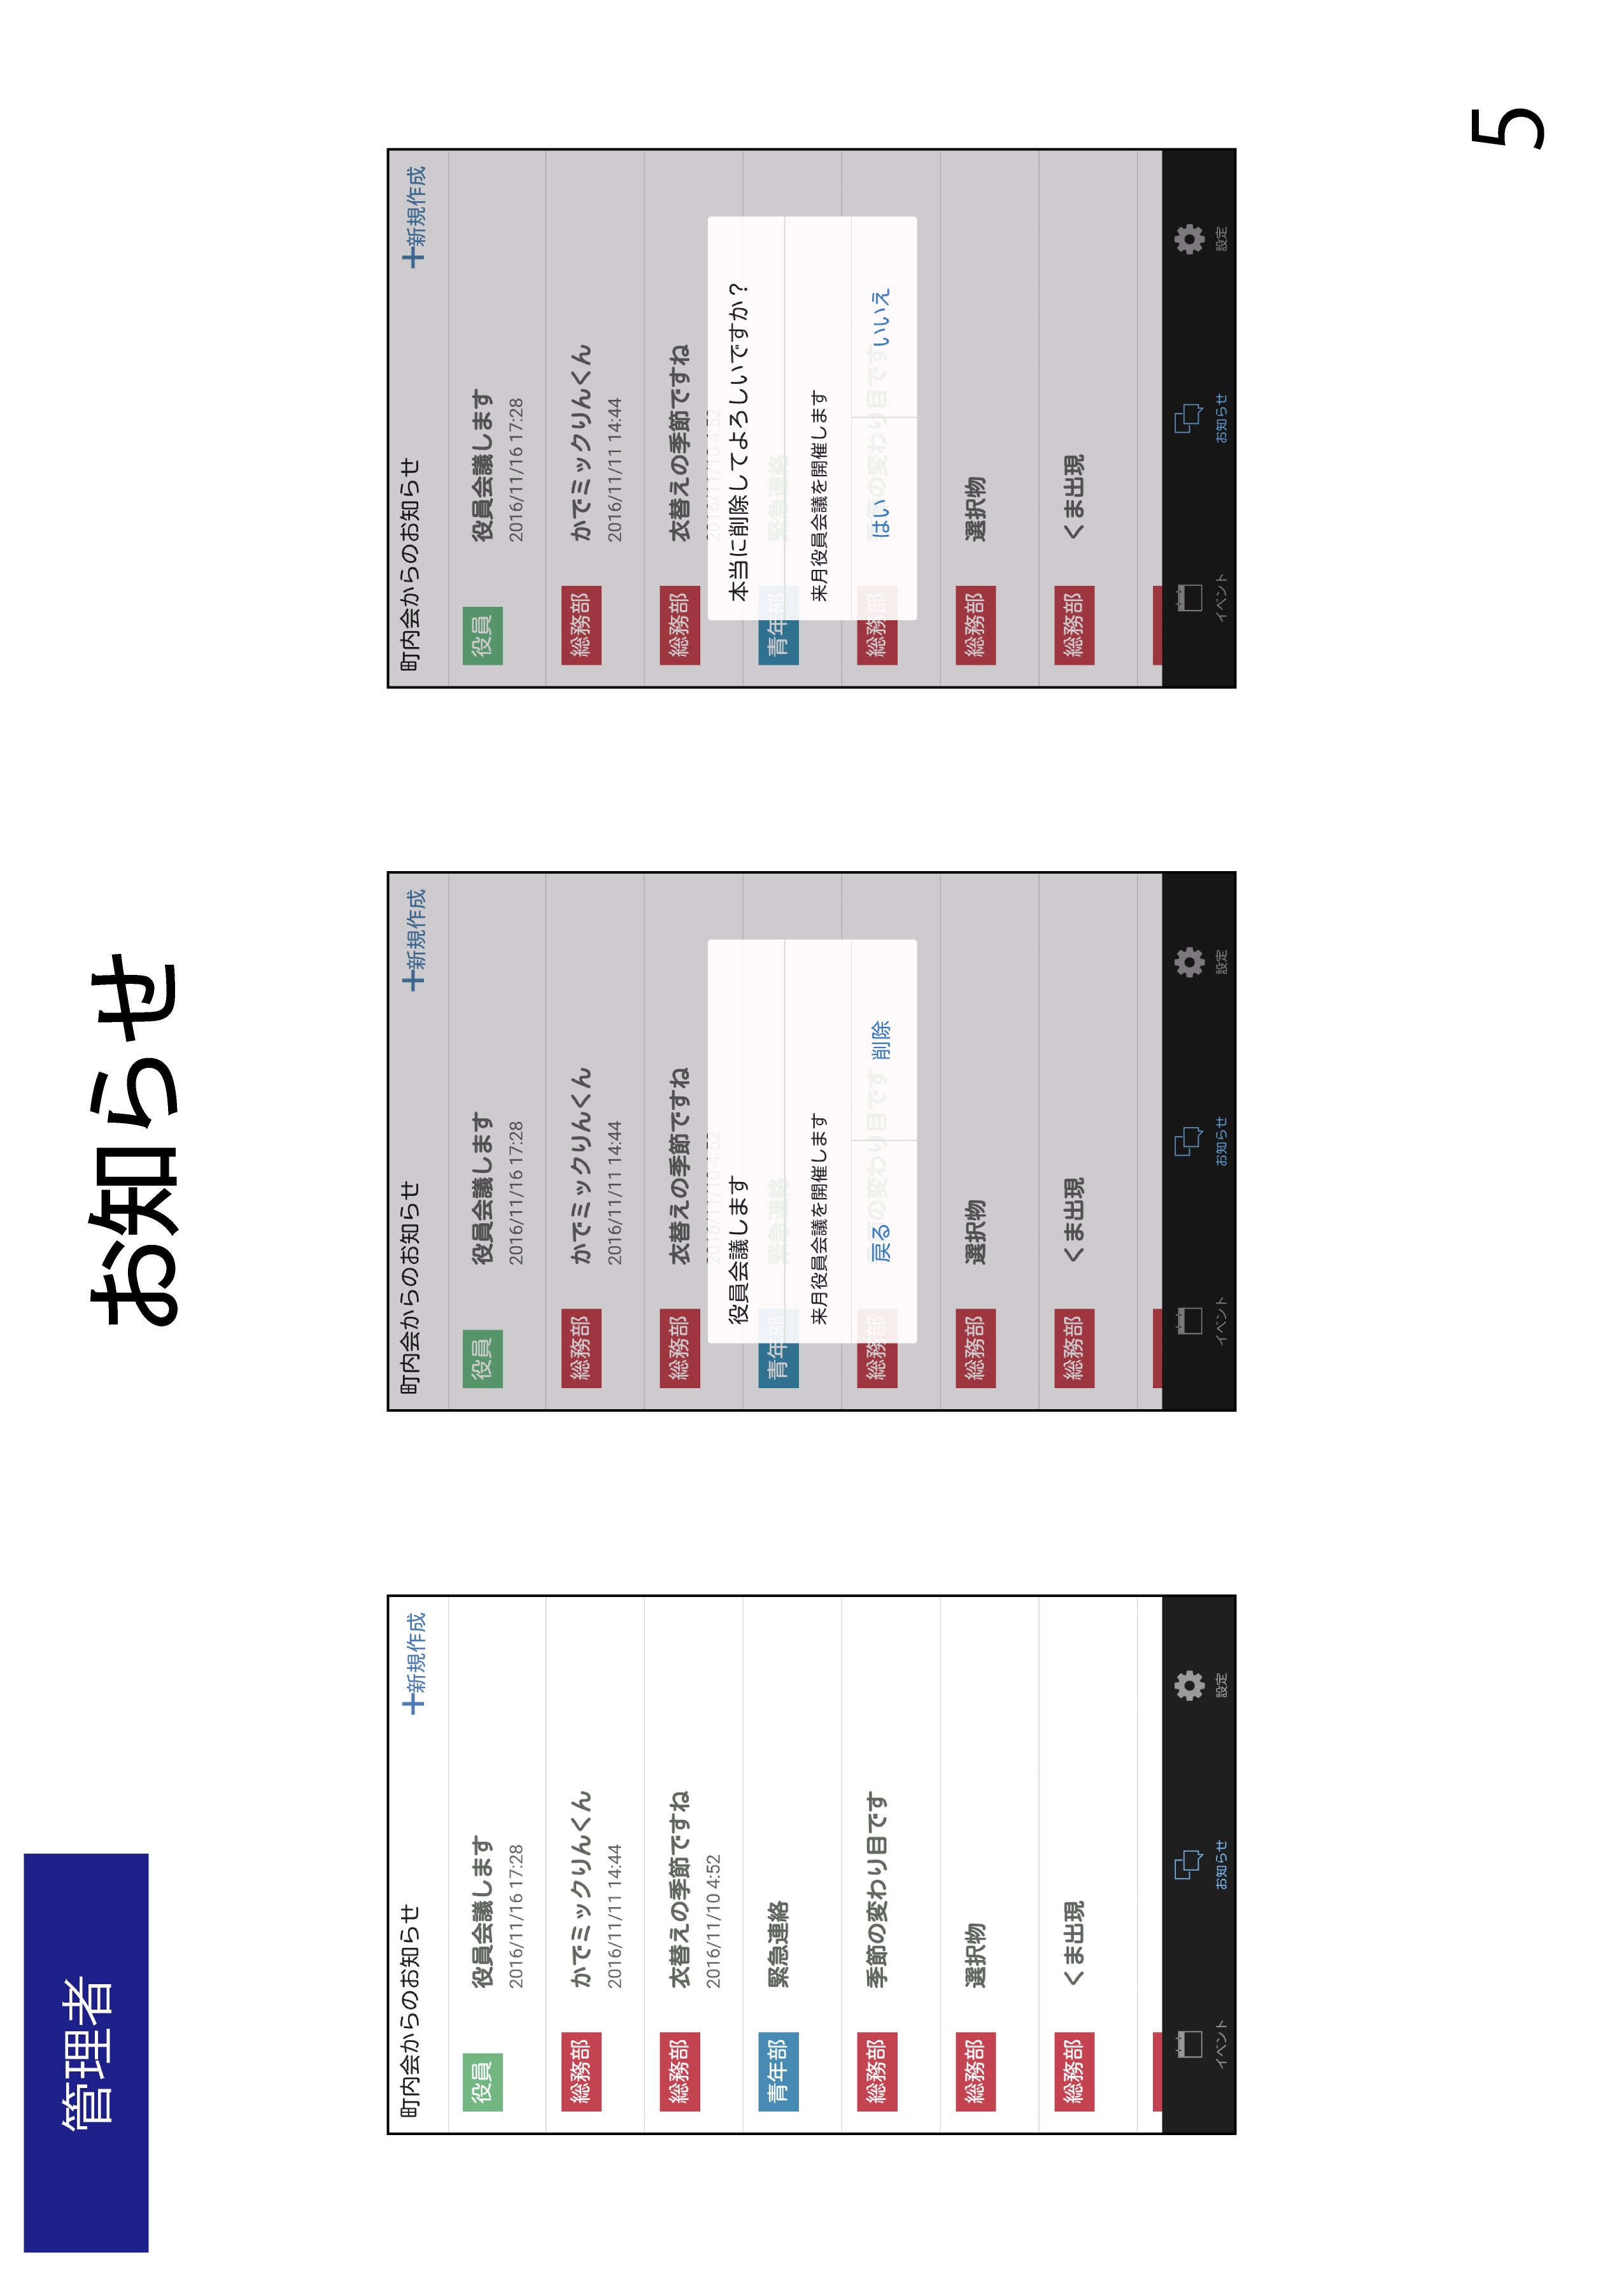
\includegraphics[keepaspectratio, scale=0.7]{appendix11_18-06.png}
    \end{center}
\end{figure}

\begin{figure}[ht]
    \begin{center}
      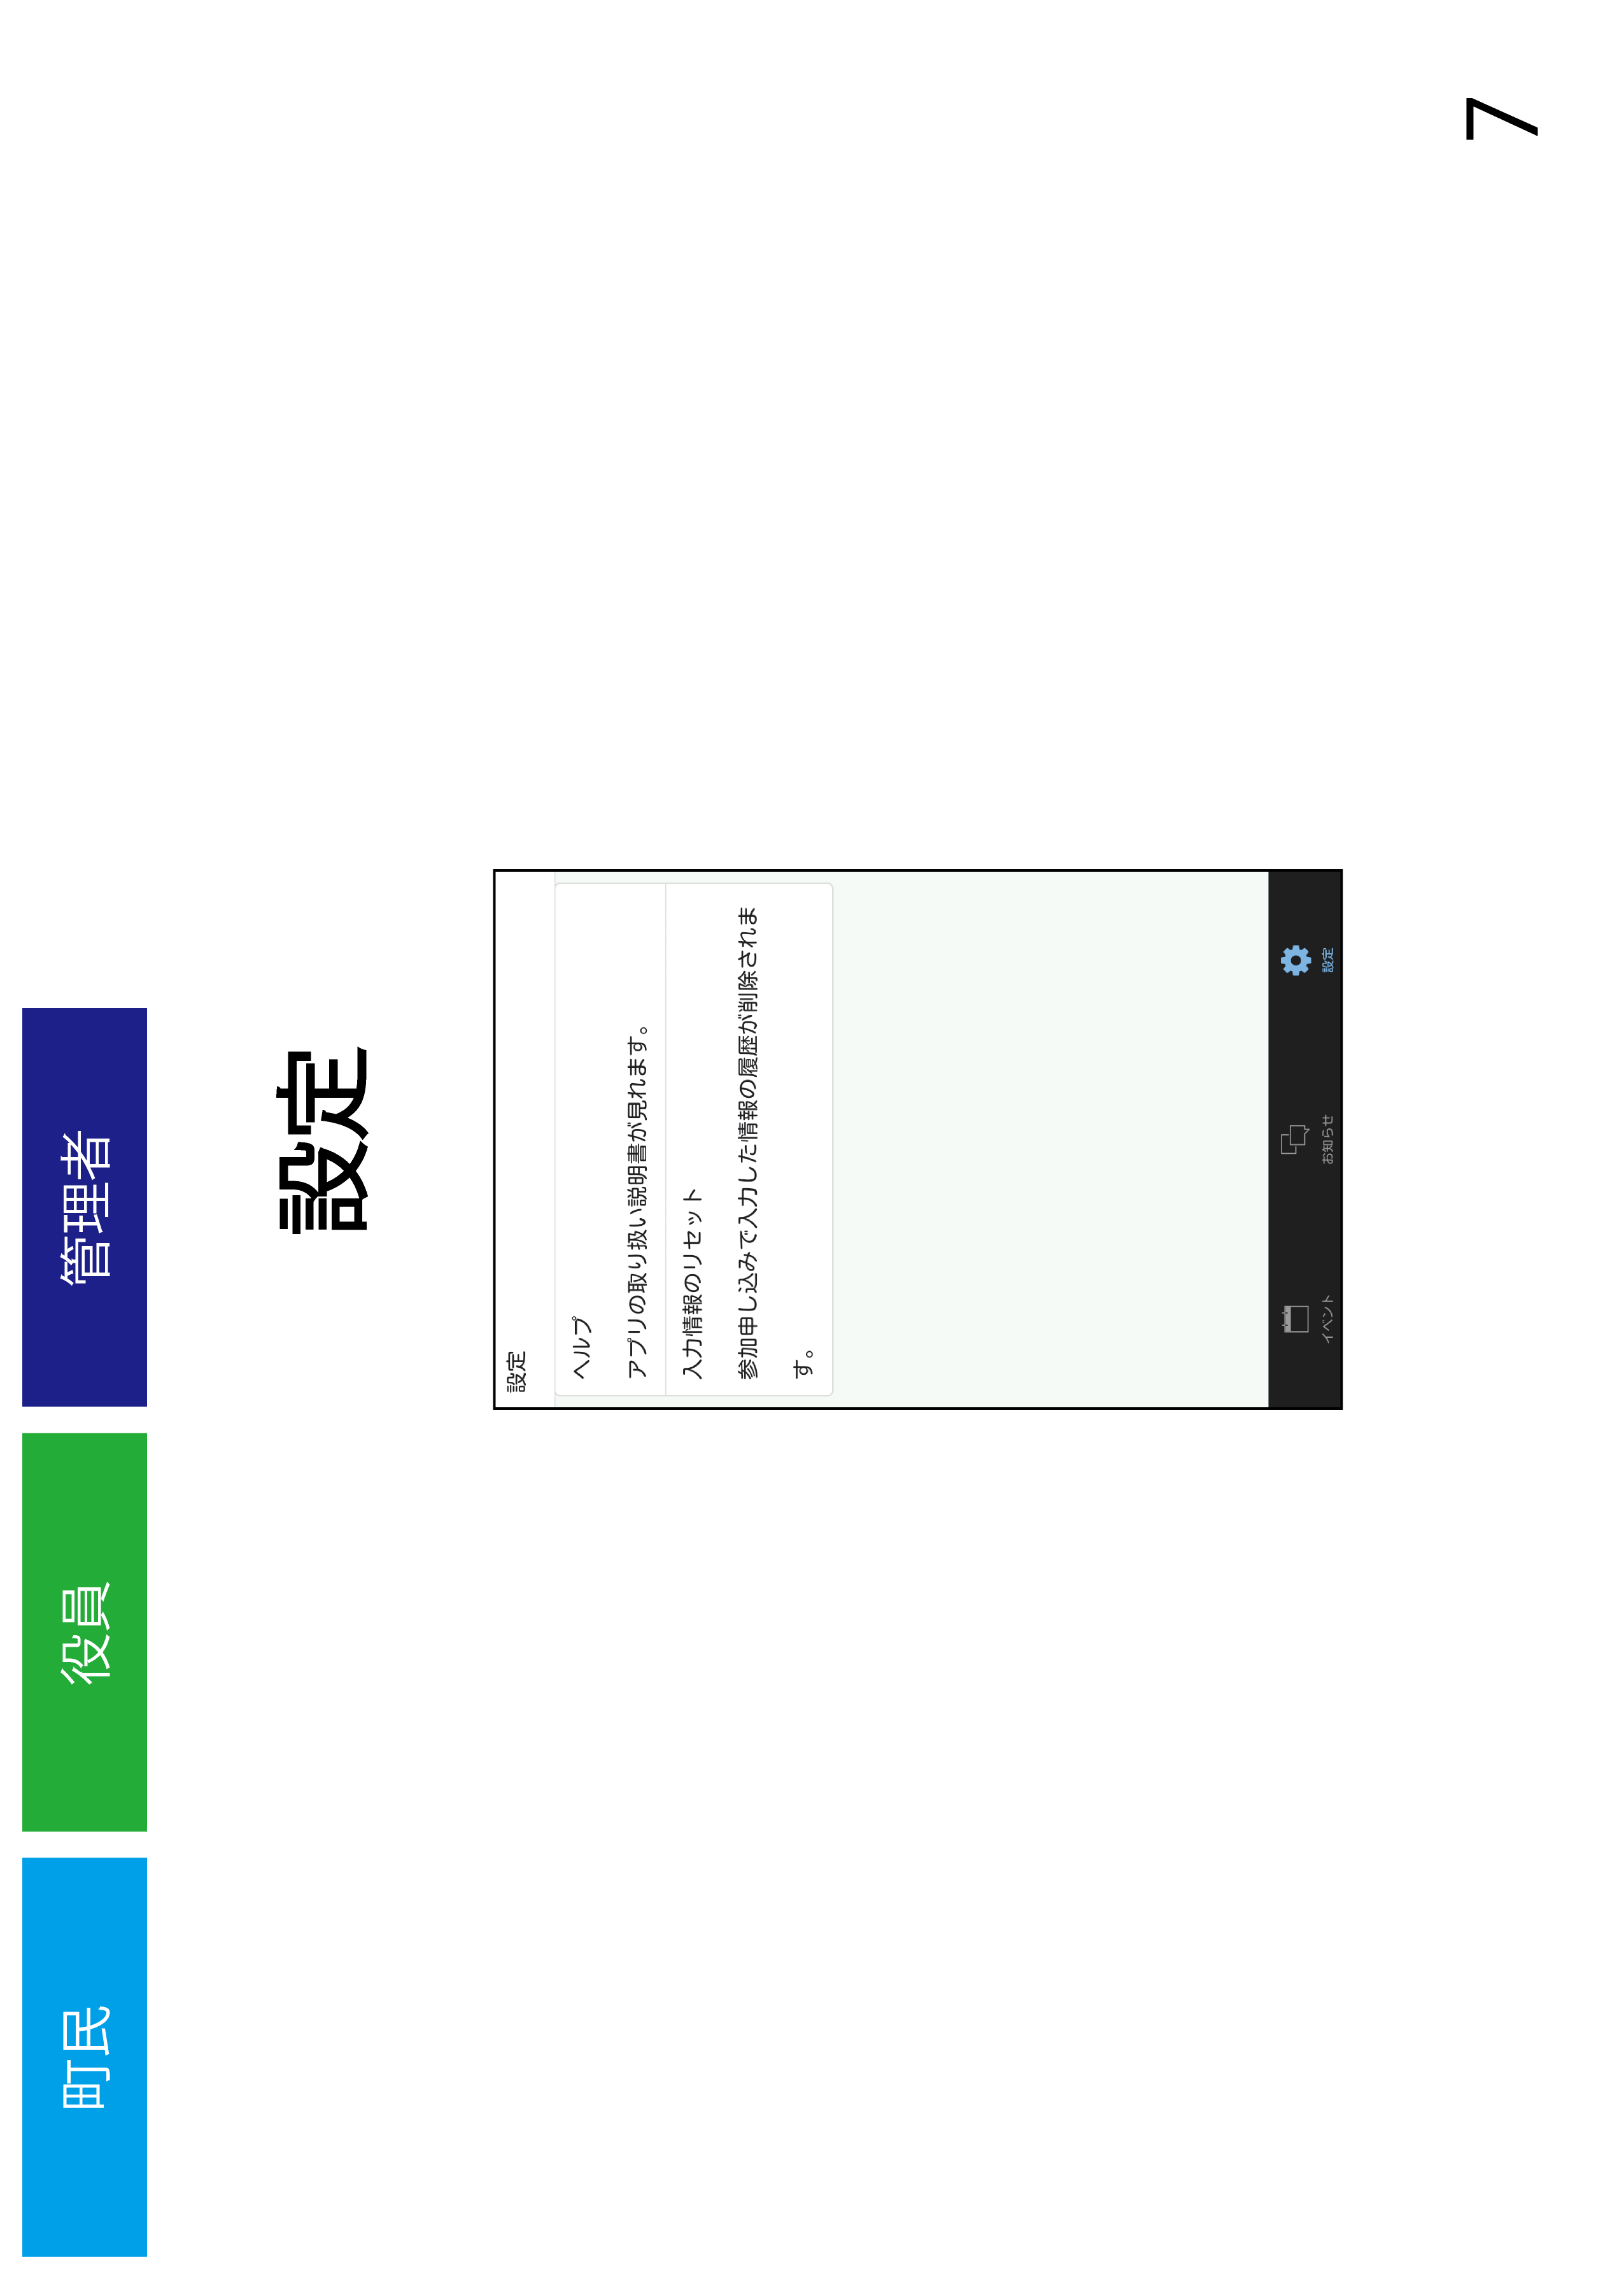
\includegraphics[keepaspectratio, scale=0.7]{appendix11_18-07.png}
    \end{center}
\end{figure}

\begin{figure}[ht]
    \begin{center}
    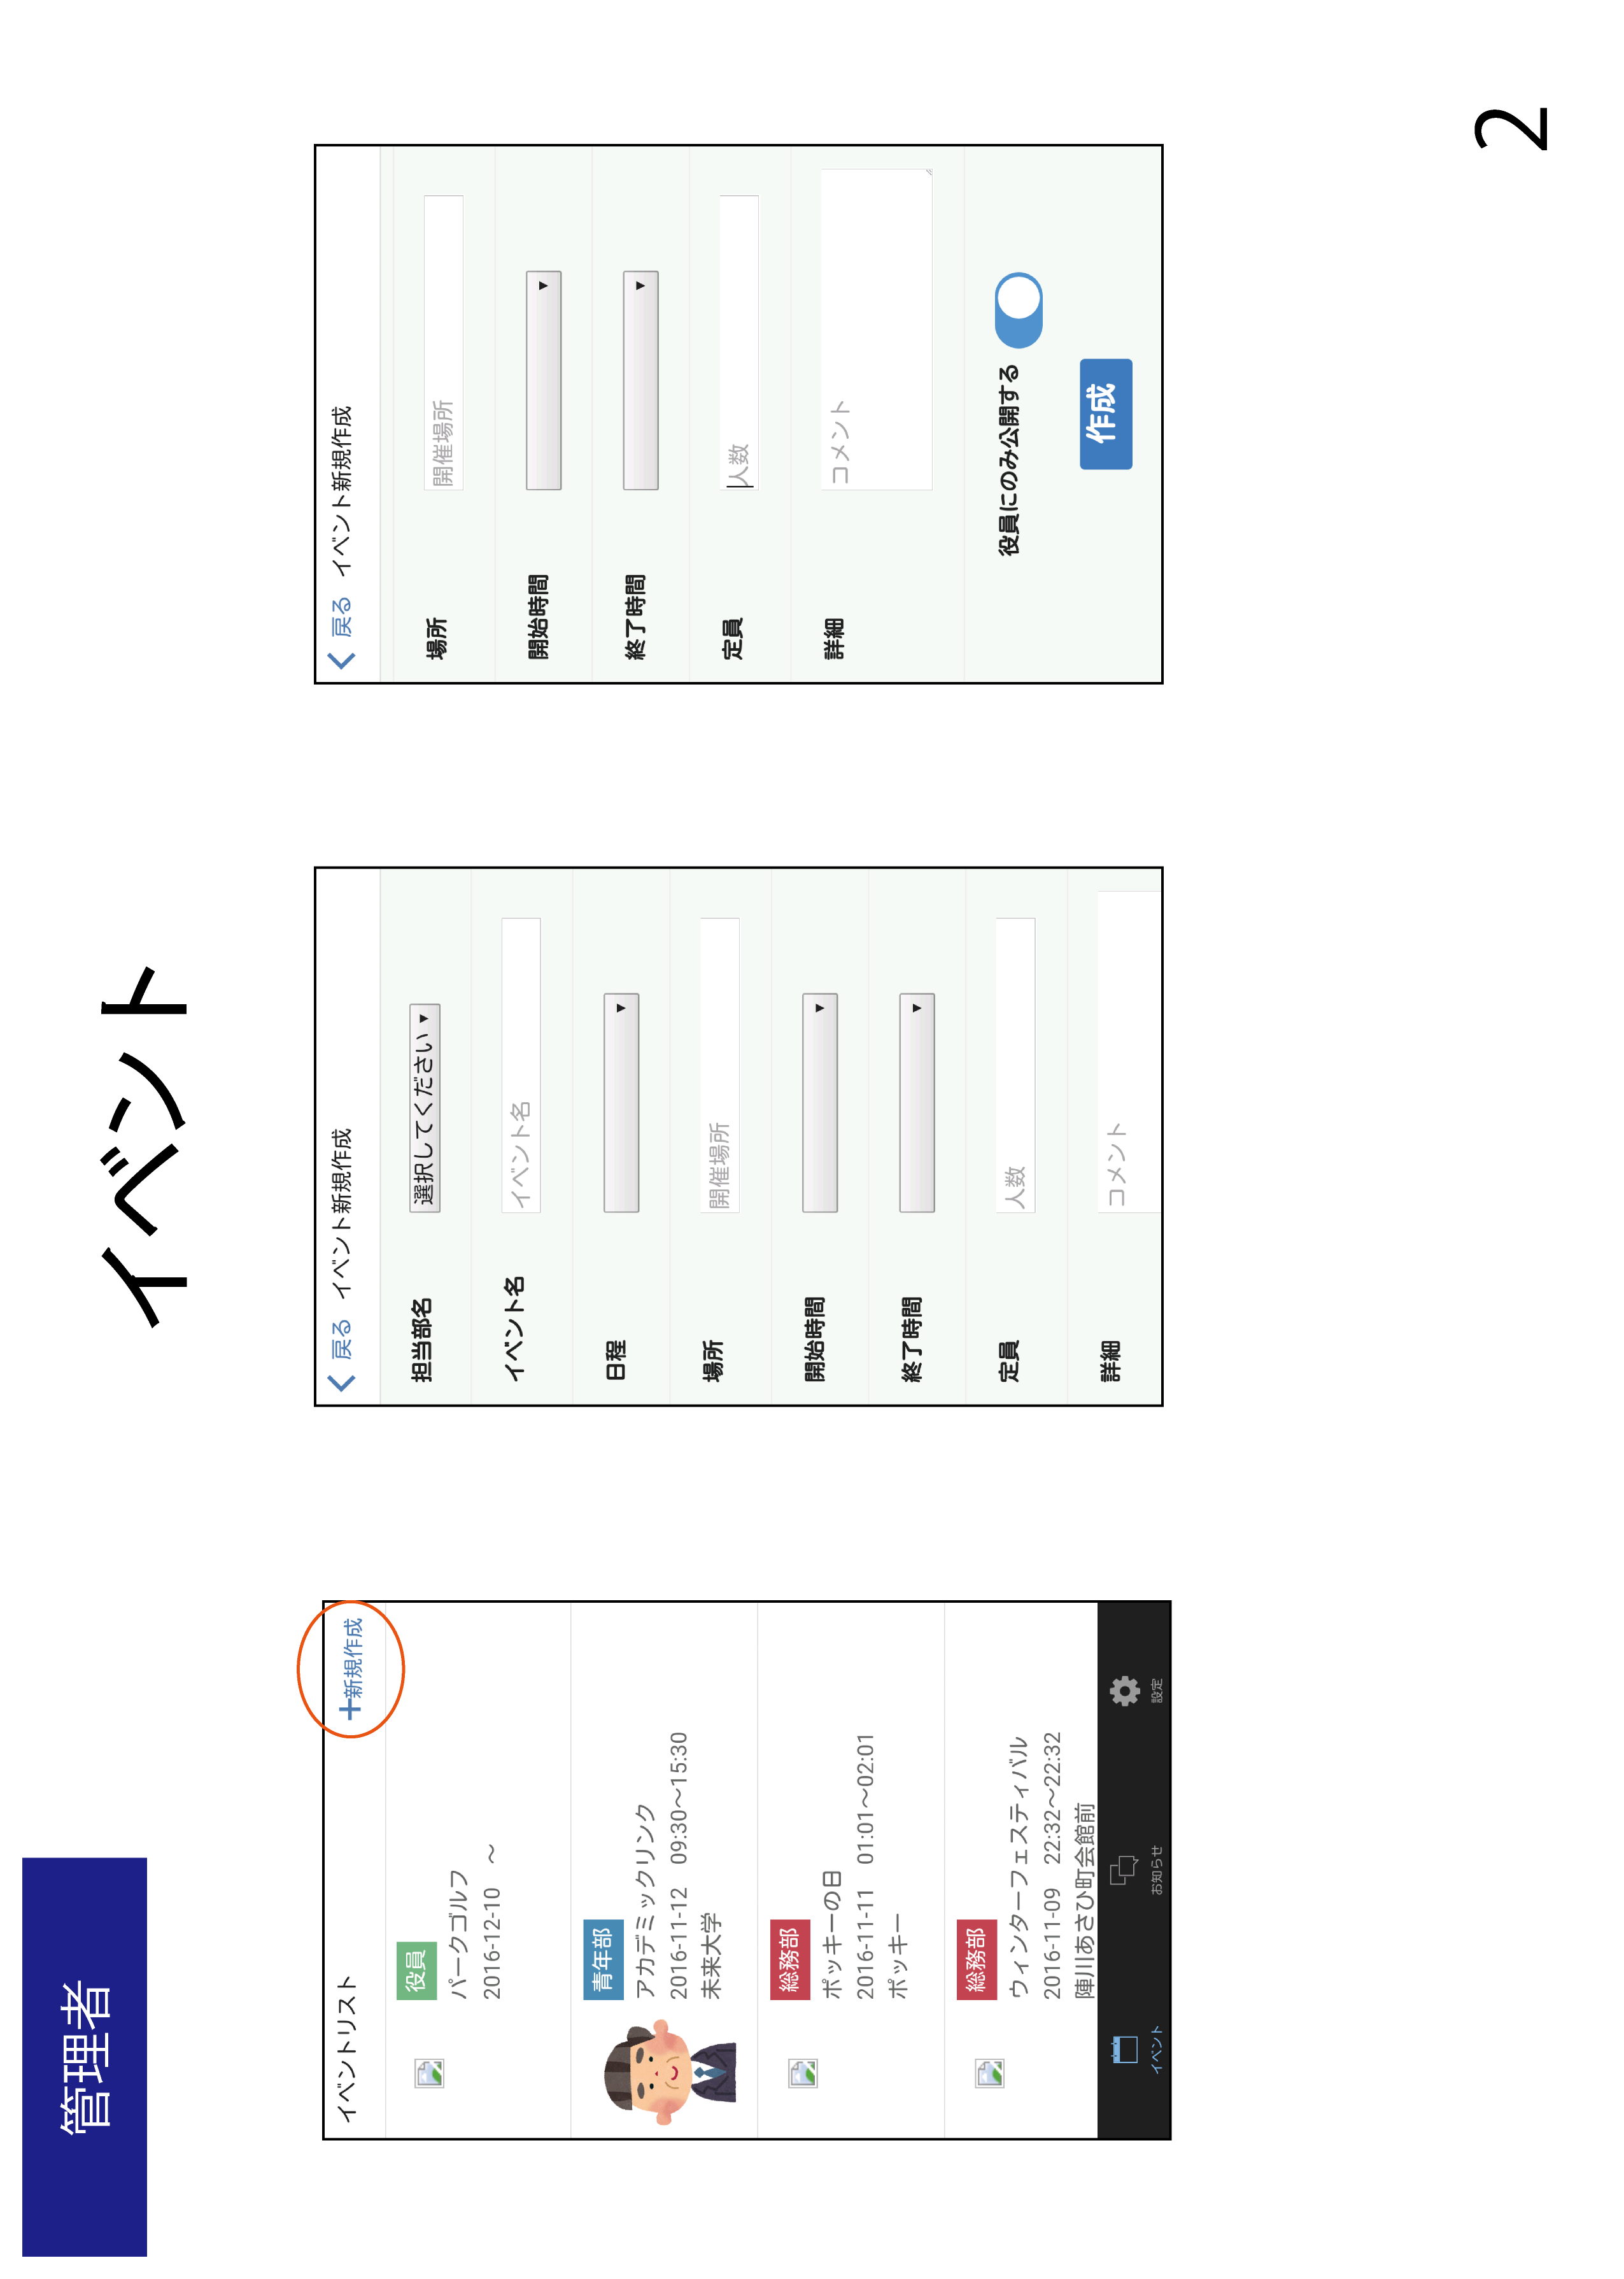
\includegraphics[keepaspectratio, scale=0.7]{appendix11_18-08.png}
    \end{center}
\end{figure}

\begin{figure}[ht]
    \begin{center}
      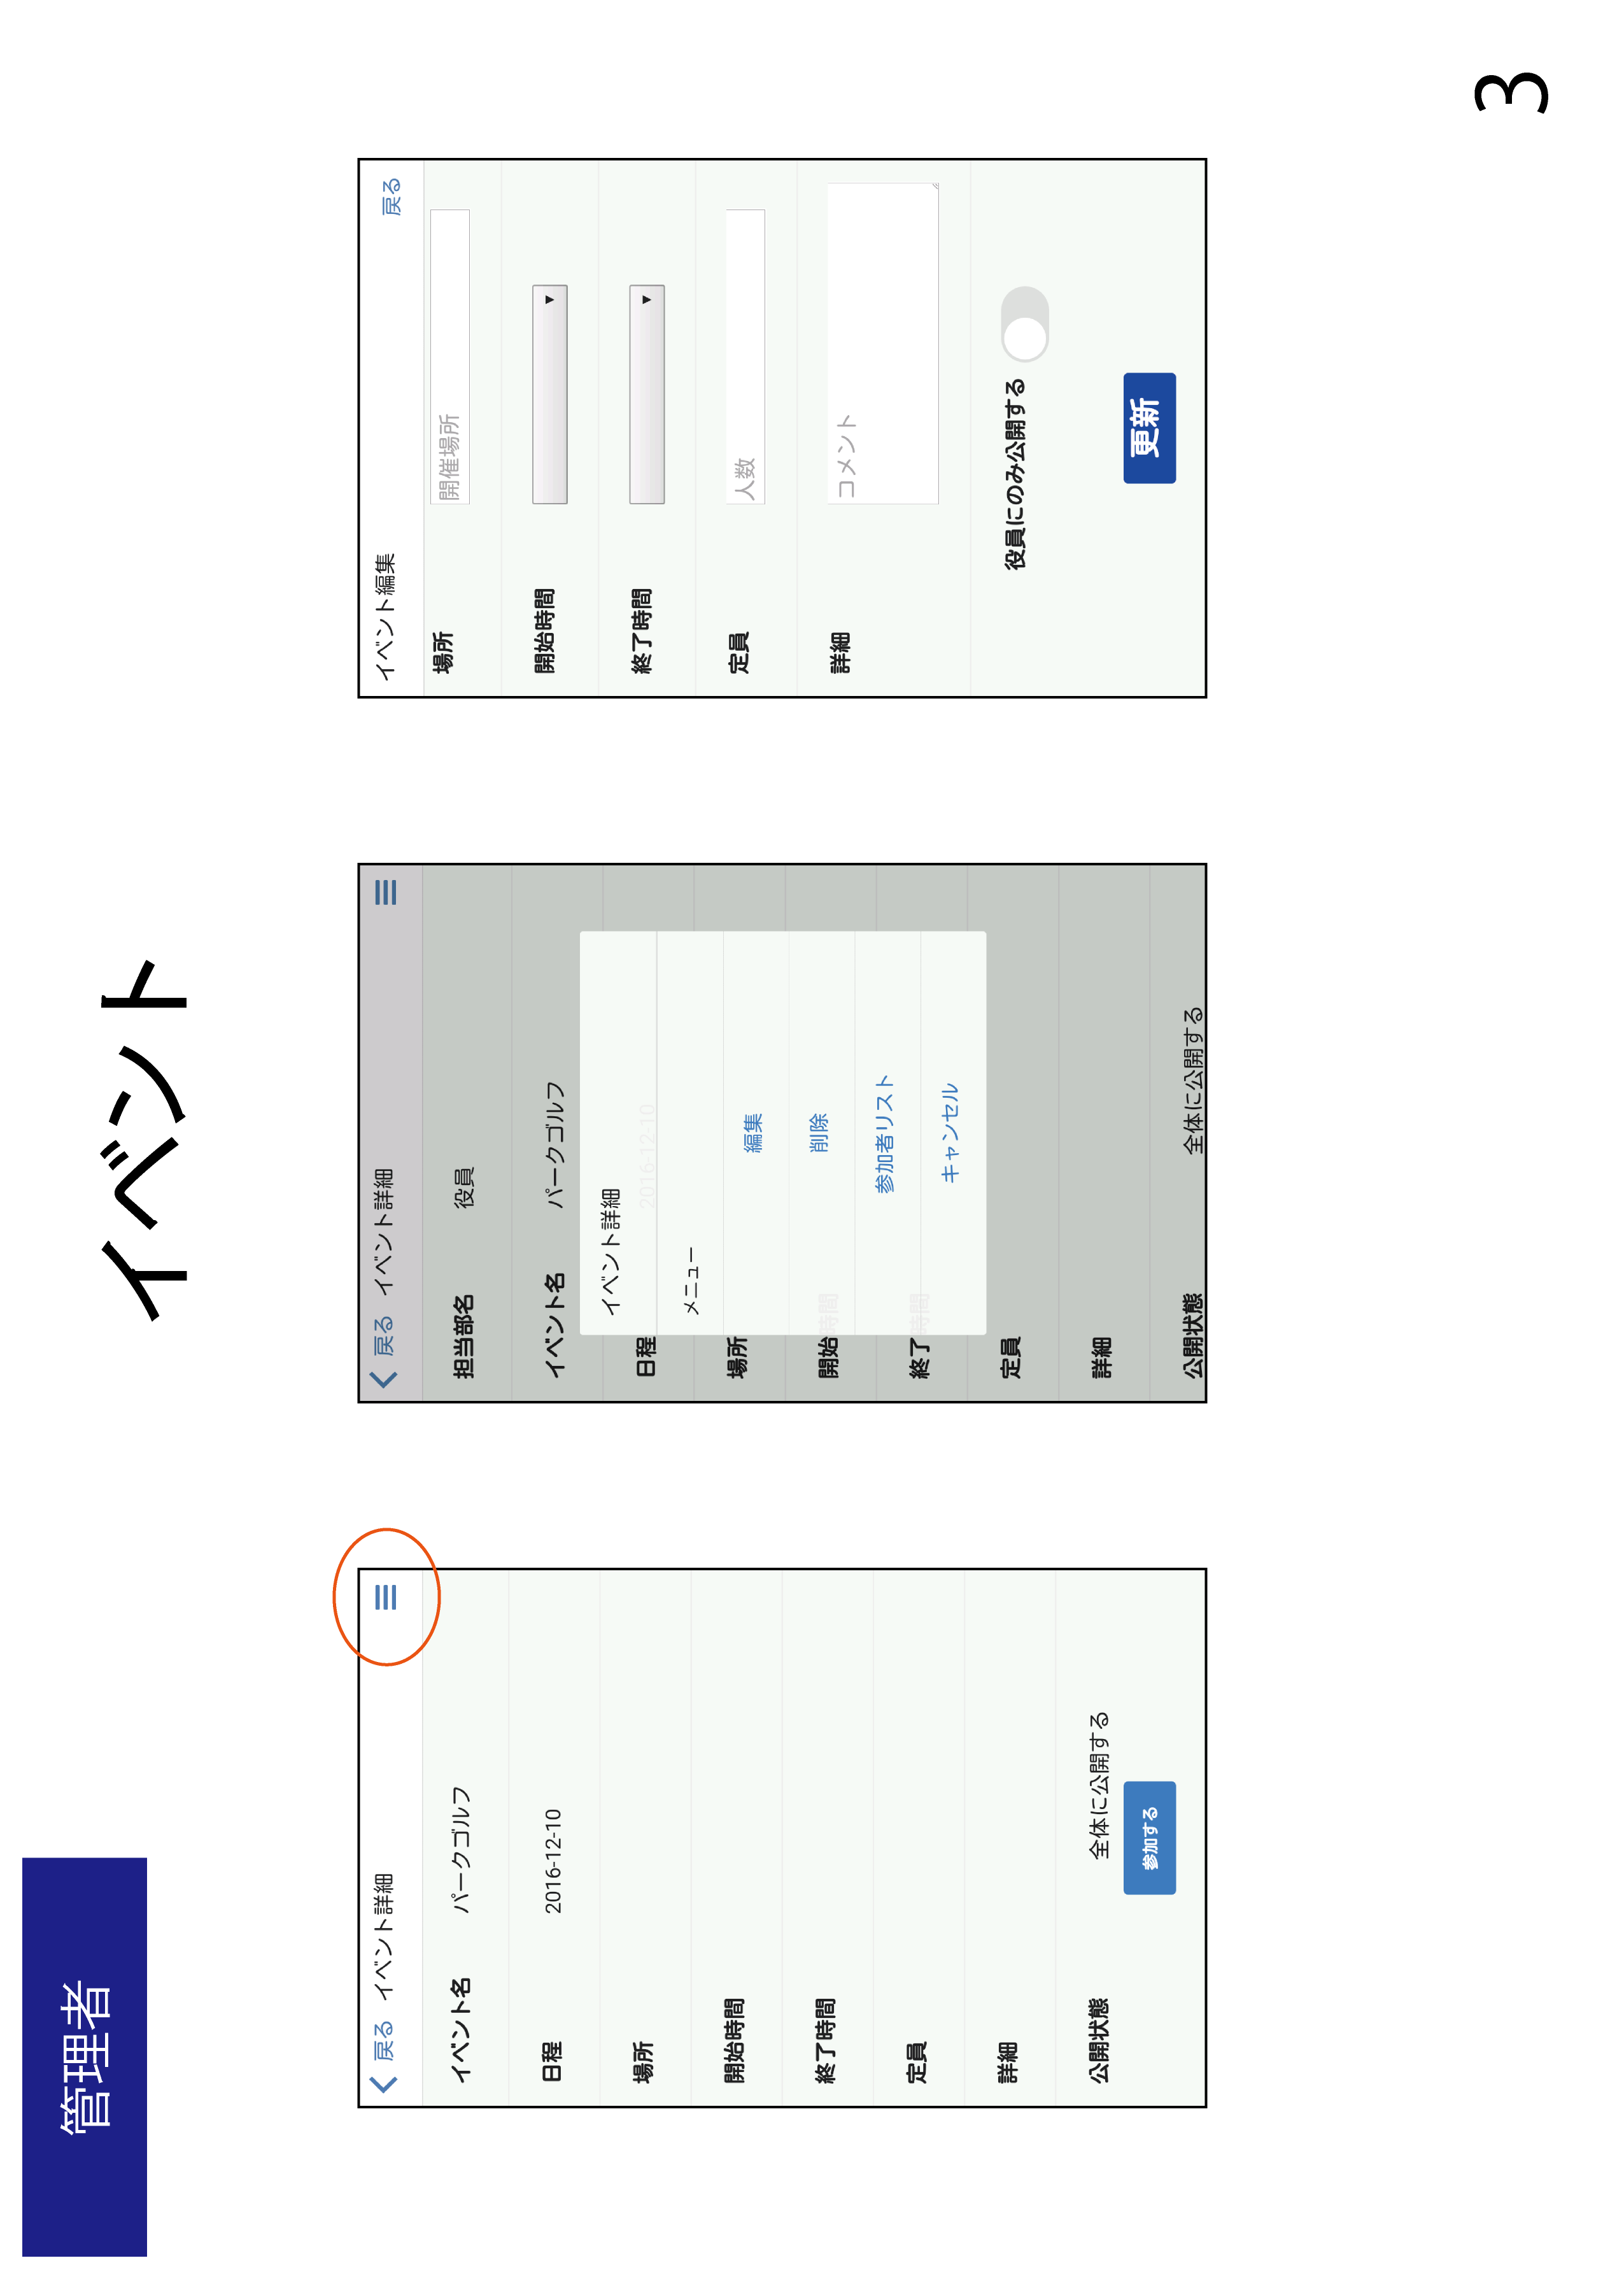
\includegraphics[keepaspectratio, scale=0.7]{appendix11_18-09.png}
    \end{center}
\end{figure}

\begin{figure}[ht]
    \begin{center}
      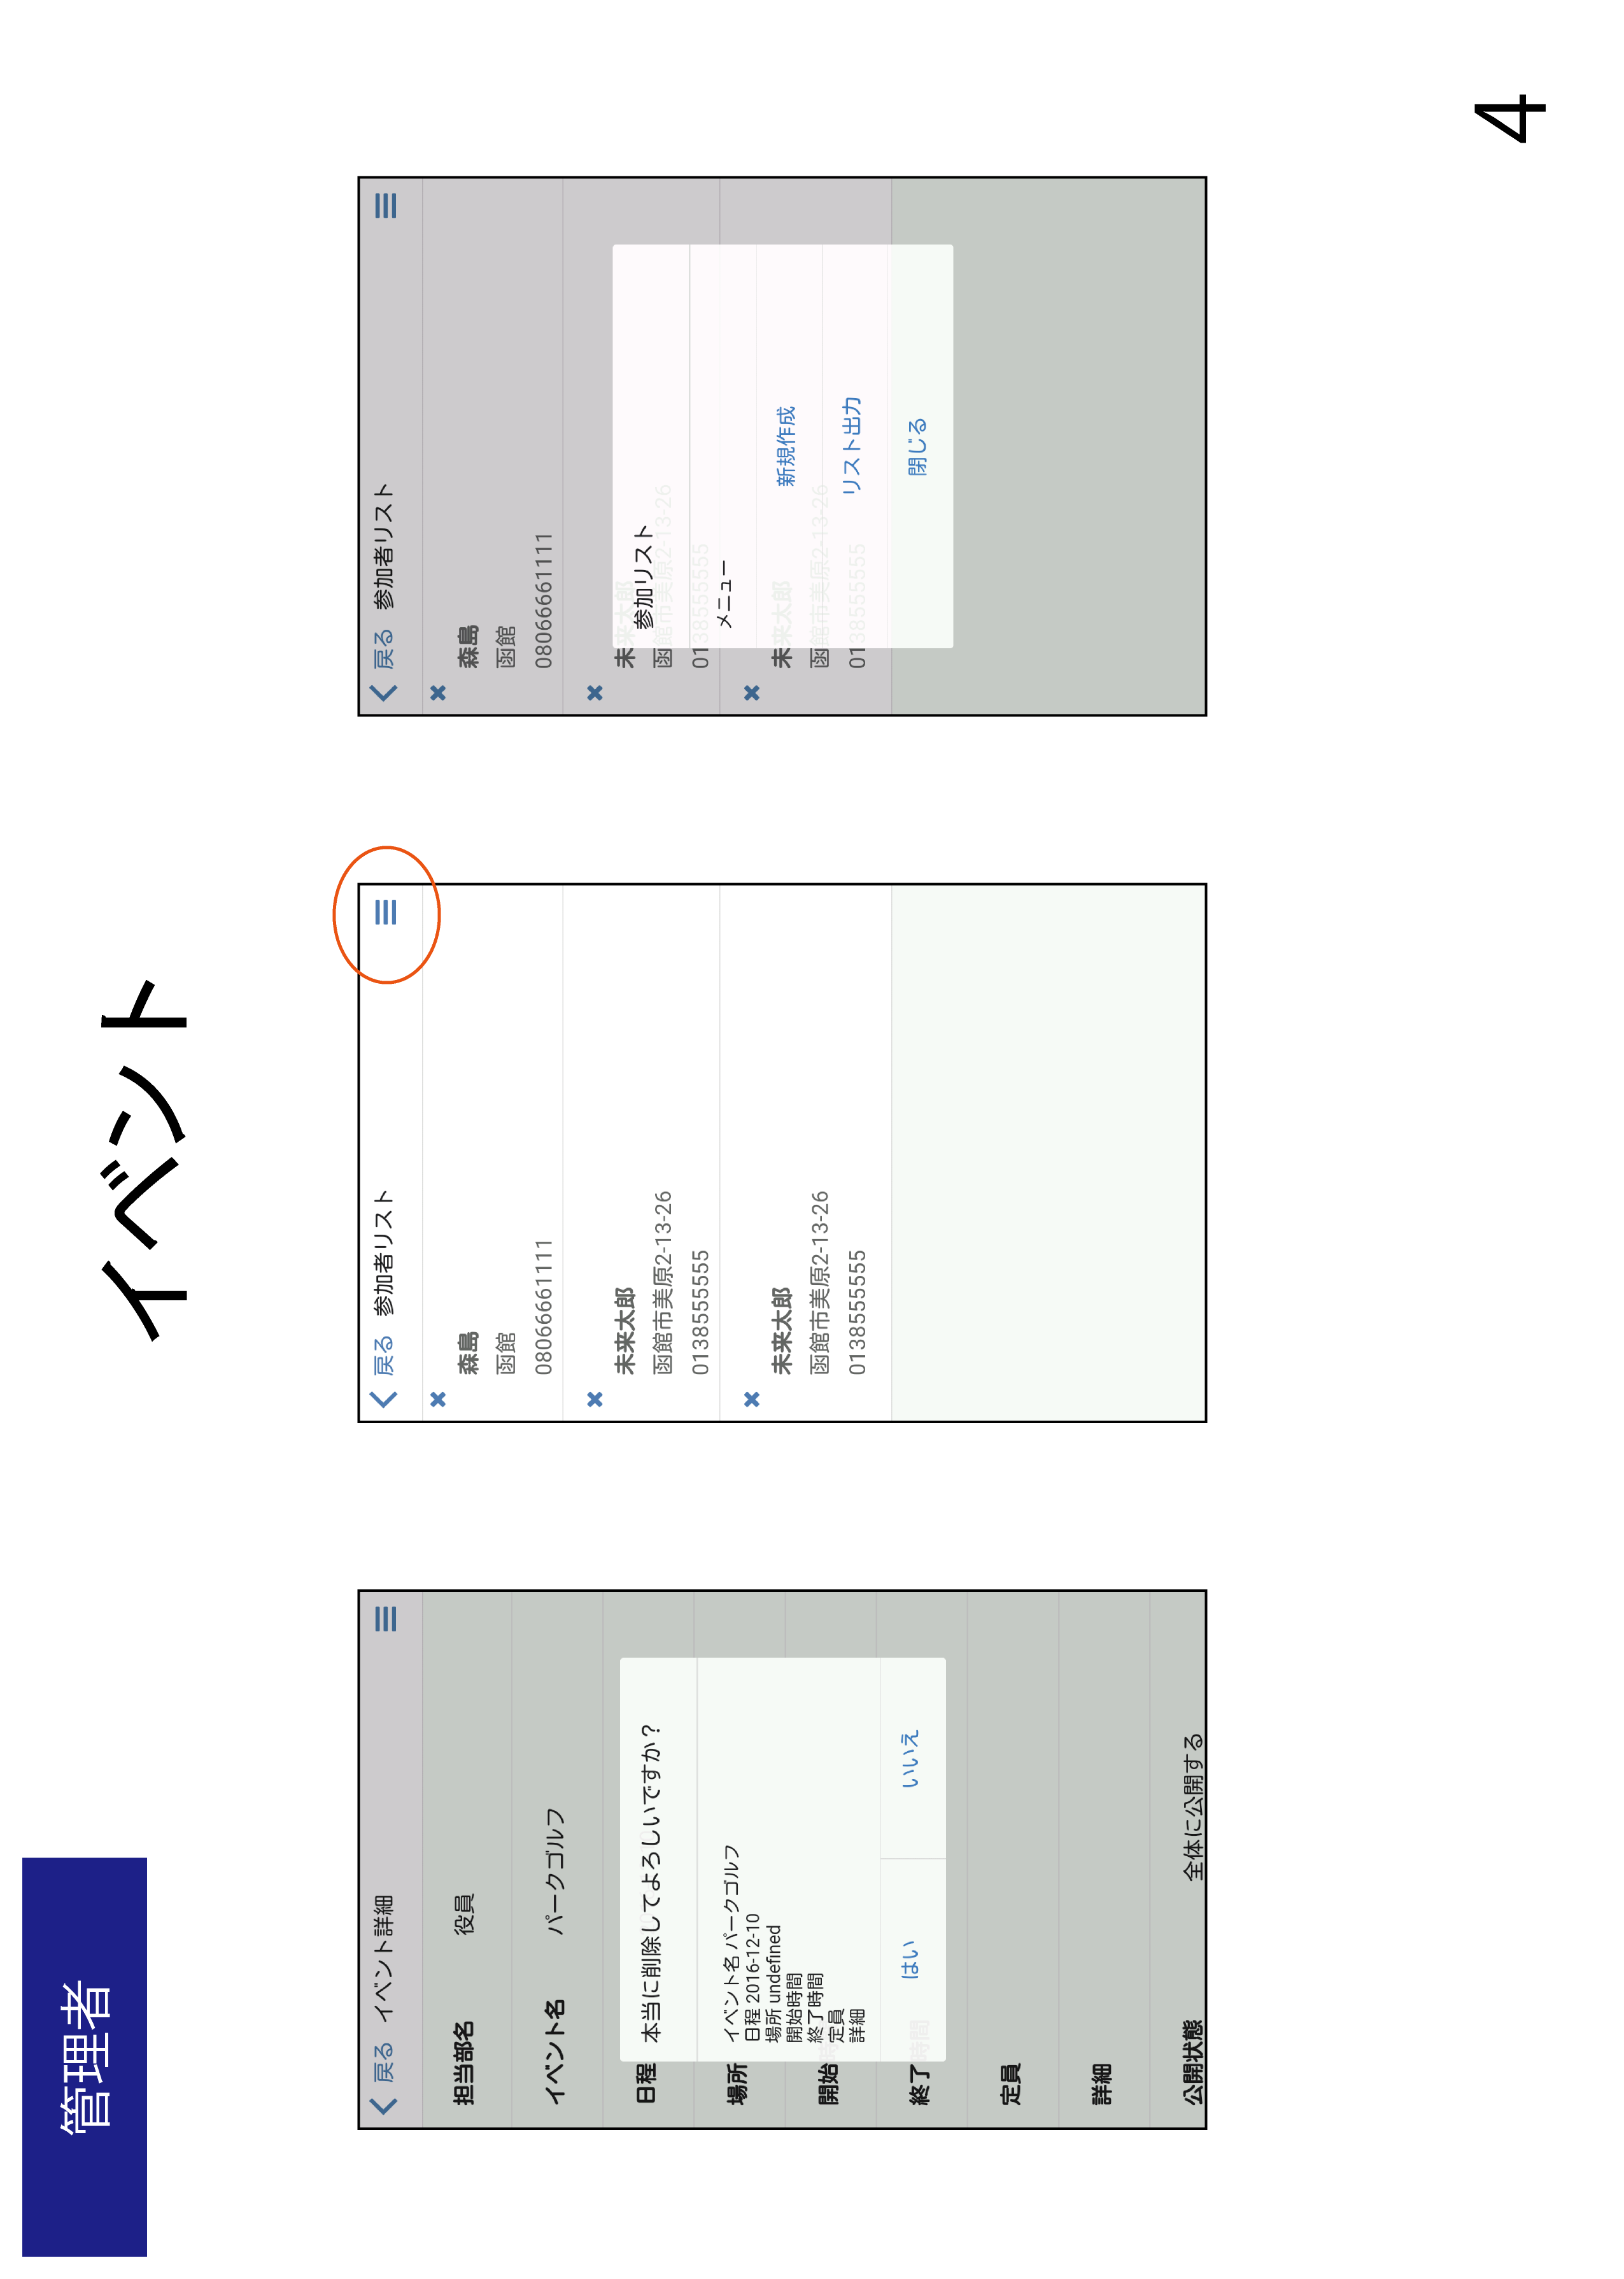
\includegraphics[keepaspectratio, scale=0.7]{appendix11_18-10.png}
    \end{center}
\end{figure}

\begin{figure}[ht]
    \begin{center}
      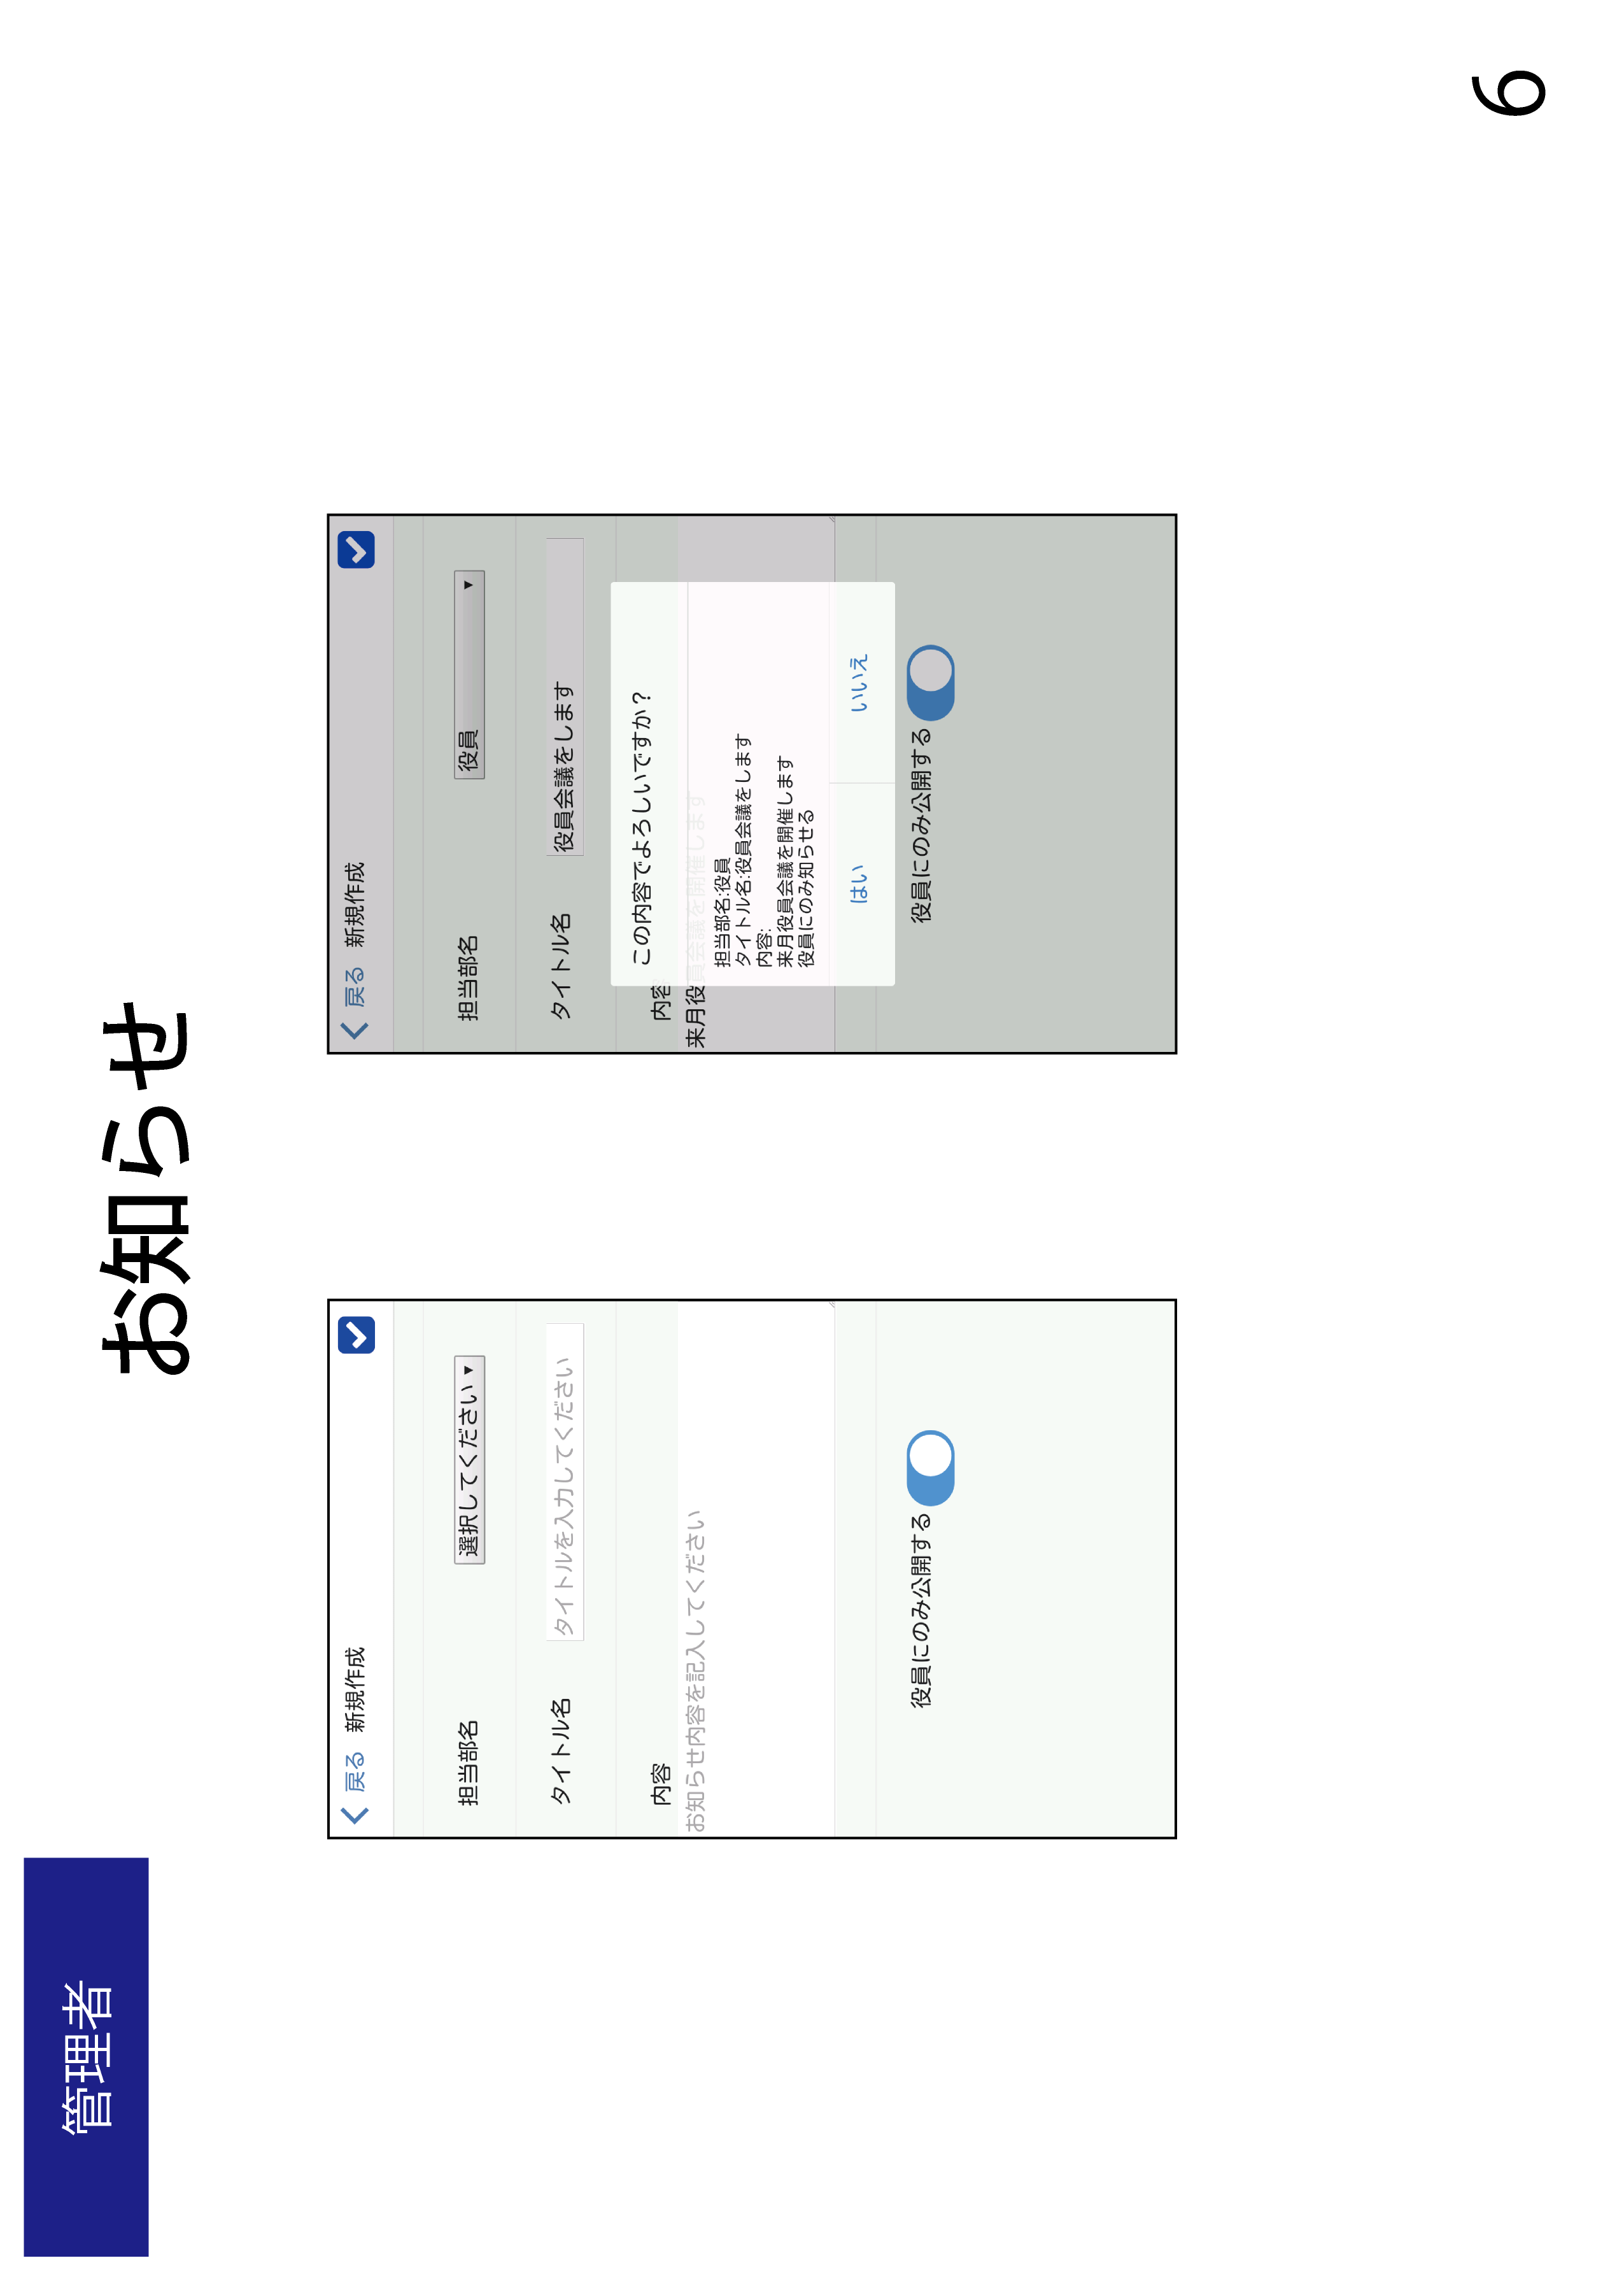
\includegraphics[keepaspectratio, scale=0.7]{appendix11_18-11.png}
    \end{center}
\end{figure}


%付録の終わり
\end{appendix}


%\backmatter

% 参考文献
\begin{thebibliography}{10}
\bibitem {book_about_monaca} 永井勝則. クラウドでできるHTML5ハイブリッドアプリ開発 Cordova/Onsen UIで作るiOS/Android両対応アプリ (Monaca公式ガイドブック) . 翔泳社, 2015.
\bibitem {monaca_debugger} Monaca. Monaca Debugger HTMLハイブリッドアプリのテストを超効率化. 2016. \url{https://ja.monaca.io/debugger.html} (2016/7/20アクセス)
\bibitem {about_mbaas} NIFTY Cloud mobile backend. mBaaSとは. 不明. \url{http://mb.cloud.nifty.com/about.htm}(2016/7/16アクセス)
\bibitem {price_mbaas} NIFTY Cloud mobile backend. 料金. 不明. \url{http://mb.cloud.nifty.com/price.htm }(2016/7/16アクセス)
\bibitem {intro_mbaas} nifty. ニフティクラウド「mobile backend」のご紹介. 不明. \url{http://lp.mb.cloud.nifty.com/mbaaspaperdownload} (2016/7/20アクセス)
\bibitem {book_about_github} 大塚弘記. GitHub実践入門 Pull Requestによる開発の変革. 技術評論社, 2014.
\bibitem {monkey_git} サルでもわかるGit入門~バージョン管理を使いこなそう~. Gitの基本 はじめに. 2014. \url{http://www.backlog.jp/git-guide/intro/intro1_1.html}(2016/7/16アクセス)
\bibitem {tutorial_monaca_CLI} Monaca. Monaca CLI チュートリアル. 2011. \url{https://docs.monaca.io/ja/quick_start/cli/ }(2016/7/16アクセス)
\bibitem {Redmine} Redline.JP. チケットのウォッチャー. 不明. \url{http://redmine.jp/glossary/i/issue-watcher/ }(2016/7/16アクセス)
\bibitem {Trello} SELECK. 無料&日本語化!「Trello」でタスク管理がラクになる!使い方・始め方を解説します. 2016. \url{https://seleck.cc/610 }(2016/12/16アクセス)
\end{thebibliography}

\end{document}
